\documentclass[a4paper,11pt]{article}

\newcommand{\XX}{\textbf{MathVRE}\xspace}
\newcommand{\TheProject}{\XX}

\usepackage{lscape} % for landscape
\usepackage{comments}
% %\usepackage[final]{comments}
\usepackage{verbatim}
\usepackage{listings}
\usepackage{supertabular,array}
\makeatletter
\newcommand\arraybslash{\let\\\@arraycr}
\makeatother
% \setlength\tabcolsep{1mm}
% \renewcommand\arraystretch{1.3}
%% Related Projects
\newcommand{\scienceproject}{\mbox{\textsc{SCIEnce}}\xspace}
\newcommand{\OOMMFNB}{OOMMF-NB\xspace}
\newcommand{\VRE}{VRE\xspace}
\newcommand{\VREs}{VRE\xspace}
\newcommand{\software}[1]{\textsc{#1}\xspace}
\newcommand{\GAP}{\software{GAP}}
\newcommand{\HPCGAP}{\software{HPC-GAP}}
\newcommand{\libGAP}{\software{libGAP}}
\newcommand{\Singular}{\software{Singular}}
\newcommand{\Sage}{\software{Sage}}
\newcommand{\SageCombinat}{\software{Sage-Combinat}}
\newcommand{\MuPADCombinat}{\software{MuPAD-Combinat}}
\newcommand{\Sphinx}{\software{Sphinx}}
\newcommand{\SCSCP}{\software{SCSCP}}
\newcommand{\Python}{\software{Python}}
\newcommand{\IPython}{\software{IPython}}
\newcommand{\Jupyter}{\software{Jupyter}}
\newcommand{\Cython}{\software{Cython}}
\newcommand{\Pythran}{\software{Pythran}}
\newcommand{\Numpy}{\software{Numpy}}
\newcommand{\Pari}{\software{PARI}}
\newcommand{\PariGP}{\software{PARI/GP}}
\newcommand{\libpari}{\software{libpari}}
\newcommand{\GP}{\software{GP}}
\newcommand{\GPtoC}{\software{GP2C}}
\newcommand{\Linbox}{\software{LinBox}}
\newcommand{\LMFDB}{\software{LMFDB}}
\newcommand{\OpenEdX}{\software{OpenEdX}}
\newcommand{\Linux}{\software{Linux}}
\newcommand{\LATEX}{\software{\LaTeX}}
\newcommand{\SMC}{\software{SageMathCloud}}
\newcommand{\Simulagora}{\software{Simulagora}}
\newcommand{\KANT}{\software{KANT}}
\newcommand{\Magma}{\software{Magma}}
\newcommand{\Mathematica}{\software{Mathematica}}
\newcommand{\Maple}{\software{Maple}}
\newcommand{\Matlab}{\software{Matlab}}
\newcommand{\MuPAD}{\software{MuPAD}}
\newcommand{\MPIR}{\software{MPIR}}
\newcommand{\Arxiv}{\software{arXiv}}
\newcommand{\Givaro}{\software{Givaro}}
\newcommand{\fflas}{\software{fflas}}
\newcommand{\MathHub}{\software{MathHub}}
\newcommand{\FindStat}{\software{FindStat}}
\newcommand\DKS{\ensuremath{\mathcal{DKS}}\xspace}

%%% Local Variables: 
%%% mode: latex
%%% TeX-master: "proposal"
%%% End: 

% Partners
\newparticipant{PS}{Université Paris Sud}{UPS}{FR}
\newparticipant{LL}{Logilab}{Logilab}{FR}
\newparticipant{UV}{Université de Versailles Saint-Quentin}{UVSQ}{FR}
\newparticipant{UG}{Université Joseph Fourier}{UJF}{FR}
\newparticipant{UB}{Université Bordeaux}{UB}{FR}
\newparticipant{UO}{University of Oxford}{UO}{UK}
\newparticipant{USH}{Université of Sheffield}{USHEF}{UK}
\newparticipant{USO}{Université of Southhampton}{USO}{UK}
\newparticipant{SA}{University of St Andrews}{USTAN}{UK}
\newparticipant{UW}{University of Warwick}{UW}{UK}
\newparticipant{UK}{University of Kaiserslautern}{UK}{DE}
\newparticipant{US}{University of Silesia}{US}{PL}
\newparticipant{ZH}{Universit\"{a}t Z\"{u}rich}{UZH}{CH}
\newparticipant{SR}{Simula Research Laboratory}{Simula}{NO}
% Participant or third party?
\newparticipant{UWS}{University of Washington at Seattle}{UWS}{US}
% Jean-Pierre Flori
% Luca DeFeo
% Jean-Guillaume Dumas
% Clément Pernet

% Personalised comments for each author
\newcommand{\slcomment}[1]{\comment{SL}{#1}}
\newcommand{\akcomment}[1]{\comment{AK}{#1}}

%% Related Projects
\newcommand{\scienceproject}{\mbox{\textsc{SCIEnce}}}


%%% Local Variables: 
%%% mode: plain-tex
%%% TeX-master: "proposal"
%%% End: 


\begin{document}

\begin{titlepage}

\begin{center}
{\Large \textbf{COVER PAGE}}
\end{center}

\begin{tabular}{llr}
\textbf{Title of Proposal:} & \textbf{\TheProject{}: Collaborative ecosystems for mathematical research and software development} & \\[2ex] % \includeimage[scale=0.5]{logo} \\
\textbf{Date of preparation:} & \textbf{\today} & \comment{}{$
$Revision: 0.0$ $}\\[2ex]
\textbf{List of participants} && \\[2ex]


\end{tabular}

\begin{center}
\begin{tabular}{|l|p{3in}|l|l|}\hline
Participant no & Participant organisation name & Country\\

\hline
1 (Coordinator) & \longparticipant{1} & \country{1}  \\ \hline
2 & \longparticipant{2} & \country{2}  \\ \hline
3 & \longparticipant{3} & \country{3}  \\ \hline
4 & \longparticipant{4} & \country{4}  \\ \hline
5 & \longparticipant{5} & \country{5}  \\ \hline
6 & \longparticipant{6} & \country{6}  \\ \hline
7 & \longparticipant{7} & \country{7}  \\ \hline
8 & \longparticipant{8} & \country{8}  \\ \hline
9 & \longparticipant{9} & \country{9}  \\ \hline
10 & \longparticipant{10} & \country{10}  \\ \hline
11 & \longparticipant{11} & \country{11} \\ \hline
12 & \longparticipant{12} & \country{12} \\ \hline
13 & \longparticipant{13} & \country{13} \\ \hline
14 & \longparticipant{14} & \country{14} \\ \hline
\end{tabular}
\end{center}

\tableofcontents

\eucommentary{Please follow the structure of this template when
  preparing your proposal. It has been designed to ensure that the
  important aspects of your planned work are presented in a way that
  will enable the experts to make an effective assessment against the
  evaluation criteria. Sections 1, 2 and 3 each correspond to an
  evaluation criterion for a full proposal.\\
  Please be aware that proposals will be evaluated as they were
  submitted, rather than on their potential if certain changes were to
  be made. This means that only proposals that successfully address
  all the required aspects will have a chance of being funded. There
  will be no possibility for significant changes to content, budget
  and consortium composition during grant preparation.\\
  Page limit: The cover page, and sections 1, 2 and 3, together should
  not be longer than 70 pages. All tables in these sections must be
  included within this limit. The minimum font size allowed is 11
  points. The page size is A4, and all margins (top, bottom, left,
  right) should be at least 15 mm (not including any footers or
  headers).  If you attempt to upload a proposal longer than the
  specified limit, before the deadline you will receive an automatic
  warning, and will be advised to shorten and re-upload the
  proposal. After the deadline, any excess pages will be overprinted
  with a ‘watermark’, indicating to evaluators that these pages must
  be disregarded.\\
  Please do not consider the page limit as a target! It is in your
  interest to keep your text as concise as possible, since experts
  rarely view unnecessarily long proposals in a positive light.}
\end{titlepage}

\newpage

\begin{draft}
\section*{Outline of Project (for Proposers)}

\TODO{This is the place for various READMEs not included in the final submission}

\subsection*{Vision}

An internal attempt at specifying our vision through short
(unsubstantiated) answers.

\begin{verbatim}
> 1) Who are we?

Lead or core developers of some of the major open source components
for pure mathematics and applications:

- Computational components: GAP, Linbox, MPIR, Pari, Sage, Singular
- Databases: LMFDB (findstat as well)
- Knowledge management: MathHub

Together with, in a larger scientific domain, lead developers for:

- Collaborative user interfaces (IPython, SageMathCloud)
- Database and Scientific Computing for the industry (Logilab)
- Numerical code optimization/parallelisation (Pythran)

> 2) What is our goal?

Building blocks with a sustainable development model that can be
seamlessly combined together to build versatile high performance
VRE's, each tailored to a specific need in pure mathematics and
application.

> 2.5) What is our strategy?

Maximize sustainability and impact by reusing and improving existing
building blocks, and reaching toward larger communities whenever possible.
E.g. factoring out our common user interface needs at the level
of IPython/Jupyter will save us time (sustainability), and impact
the larger scientific computing community.
The improvements to the building blocks will impact all their users,
whether they use the VRE or not.

> 3) From where do we start?

- Building blocks with a sustainable development model
- Proof-of-concept prototypes of VRE (SMC, Simulagora)
- Experience on combining together some of the building blocks

> 4) How do we connect or differ from other projects?

The other projects focus on either one or a few of the building
blocks, or on a specific VRE.

We articulate our work with each of them.

> 5) Why are we excellent?

The consortium puts together recognized experts in all
areas and most building blocks that are relevant to the goal. There is
simultaneously a variety of point of views and a record of past
experiences collaborating together at smaller scale
(e.g. GAP-Singular). The approach is bottom up.  Most joint tasks
consist in bringing together people with a common need. There is
experience in community building.  Most participants are
simultaneously users and developers of their tools.

All of this makes me confident that we will indeed be able to
productively collaborate. And do stuff that is first class and useful.

On Sat, Dec 13, 2014 at 11:18:10PM +0100, Wolfram Decker wrote:
> 0) What precisely is our starting point and why are we the right people to
> achieve what we promise to do? Are we leaders in the area touched
> by the proposal? How do we connect? Is there some past
> collaborative success?
> 1) You still do not say what we actually will provide. What precisely will
> the VRE offer to its users?

I more or less answered those points above. Let me know if I should
elaborate.

> Who will be its users? Will those already familiar with the involved
> CAS use it? Will it make the CAS more attractive for a much larger
> community?

One objective is definitely to make CAS and others more attractive by
lowering a lot the entry barrier to access the soft (and db, ...). A
typical situation that most of us ran into is, when collaborating with
other less tech-savvy mathematicians, to have trouble sharing code,
data, and in-the-writing papers with them. SMC was launched with this
idea in mind, and the success proves the concept.

At the same time, the improvements in the building blocks will also
impact CAS users that are happy with their current user interface /
work-flow.

Improvements to IPython will impact a much larger community.

> 2) You motivate what we wish to do by the success of SageMathCloud.
> But why do we than need another VRE? How do we differ from
> SageMathCloud?

There is no one-size-fits-all VRE. One might want to run a VRE on
one's own computer resources for a variety of reason (speed of access,
specific resources, privacy, independence, ...). One might want a
different combination of software (e.g. a lightweight VRE with only
Singular).  One might want to focus on data with LMFDB-style database
searches, or on interactive computing, or on document writing, or some
combination thereof.

> Do we have a chance to compete? Or will we rather join forces? In
> which way?

We join forces (the plan is to have William/UW in the consortium, as
non funded participant). SMC focuses on one specific cloud based
VRE. We focus on the building blocks and the glue. Both project are
mutually beneficial. See the language p. 14 of the proposal.

> 3) You motivate what we wish to do by the success of LMFDB. But what
> are our connections to this database? Will we enhance it? Will we connect
> it to other stuff we do? Will we create other databases?

LMFDB is a prototype of large scale database. We want to make it
easier for other groups of mathematicians to setup similar databases
in their area. Reciprocally, like SMC, the LMFDB with benefit back
from the improved building blocks.

> 4) Why is Europe in the lead if there is already SageMathCloud?
> Where precisely is Europe in the lead?

Europe is the lead in many of the building blocks.
\end{verbatim}

% \subsection*{Mission statement for the grant}

% Our mission is to promote the next generation of community-developed
% open source software, databases, and services adapted to the needs of
% collaborative research in pure mathematics and applications.

% Our research will cover a wide variety of aspects, ranging from
% software development models, user interfaces \TODO{virtual
%   environments?}, deployment frameworks and novel collaborative tools,
% component architecture, design, and standardization of software
% \TODO{system?} and databases, to links to publication, data archival
% and reproducibility of experiments, development models and tools, and
% social aspects.

% It will consolidate Europe's leading position in computational
% mathematics and build on the remarkable success of the ecosystem of
% projects GAP, Python/Sage, Pari, Singular, LMFDB.

\subsection*{Description of the call}

\verbatiminput{call_description}

% \TODO{What do we mean by ``new generation''}.

\renewcommand{\thepage}{\arabic{page}}
\setcounter{page}{1}
\black
\cleardoublepage
\end{draft}

%%% Local Variables: 
%%% mode: latex
%%% TeX-master: "proposal"
%%% End: 

%  LocalWords:  verbatiminput renewcommand thepage setcounter cleardoublepage


% ---------------------------------------------------------------------------
%  Section 1: Excellence
% ---------------------------------------------------------------------------

\section{Excellence}

The focus of \TheProject is on promoting community-developed open
source software, databases, and services adapted to the needs of
collaborative research in pure mathematics and applications.

It will consolidate Europe's leading position in computational
mathematics and build on the remarkable success of the ecosystem of
projects like \GAP, \Python, \Sage, \Pari, \Singular, \LMFDB.

The development of effective, flexible and easy-to-use VRE technology
is especially important for mathematicians, because their research
groups tend to be small and can be isolated.

\TODO{Reference this last claim? Maybe expand a little more,
or justify later}

\subsection{Objectives}
\label{sect:objectives}

\eucommentary{1-2 pages}
\eucommentary{\emph{Describe the specific objectives for the project,
which should be clear, measurable, realistic and achievable within the
duration of the project. Objectives should be consistent with the expected
exploitation and impact of the project (see section 2).}}




\begin{enumerate}[\textbf{Aim} 1:]
\item \label{aim:collaboration} Improve the productivity of
  researchers by promoting collaborations based on mathematical
  \emph{software}, \emph{data}, and \emph{knowledge}.
\item \label{aim:vre} Make it easy for teams of
  researchers of any size to setup custom collaborative Virtual Research
  Environments adapted to their needs and workflow, supporting the
  entire life-cycle of computational work in mathematical research,
  from initial exploration to publication, teaching and outreach.
  % and bridge the gaps between
  % code, published results, and educational material.
\item \label{aim:sharing} Enable and encourage best practice in
  computational mathematical research, including making results
  easily reproducible, making software sustainable, reusable and
  easily acessible and
  sharing data in a semantically sound way.
\end{enumerate}



Our research will cover a wide variety of aspects, ranging from
software development models, user interfaces \TODO{virtual
  environments?}, deployment frameworks and novel collaborative tools,
component architecture, design, and standardization of software
\TODO{system?} and databases, to links to publication, data archival
and reproducibility of experiments, development models and tools, and
social aspects.


The concrete objectives of \TheProject are:
\begin{enumerate}[\textbf{Objective} 1:]
\item\label{objective:framework} To develop and standardise
  an architecture allowing a range of mathematical and
  data and software components to be combined 
  with off-the shelf non-mathematical infrastructure to produce
  specialised VREs for different research communities. The
  architecture will take the form of standards documents and APIs
  eqipped, where appropriate with formal or informal mathematical
  semantics to ensure interactions are mathematically sound. This primarily
  addresses aim \ref{aim:vre}, thereby contributing to aims
  \ref{aim:collaboration} and \ref{aim:sharing}. \TODO{This is a bit long}

\item\label{objectives:core} To develop open source core components
for such VREs where existing software is not available.These
components should support VREs running
 on a variety of
  platforms, including standard e-infrastructures. This primarily
  addresses aim \ref{aim:vre}, thereby contributing to aims
  \ref{aim:collaboration} and \ref{aim:sharing}.
  


\TODO{Urgent talk to EPCC re e-infrastructure standards}

\TODO{SL Write detailed description}

\item \label{objective:community}Community building

  Bring together the communities (IPython, \Sage, \Singular)

\TODO{NT expand and write detailed description}
\item \label{objective:updates} Update a range of existing open source
  mathematical software for seamless deployment and efficient
  execution within the VRE architecture of objective \ref{objective:framework}
  This fulfills part of Aim~\ref{aim:vre}.

\TODO{SL: write detailed description}

  % Our tools will span the entire life-cycle of a research idea, . They will. This
  % project is based on existing, proven open source technologies
  % developed by our team over the last decade that have been widely
  % adopted in academia and industry.
\item \label{objective:social}Explore the social aspects: how do researchers collaborate in
  Mathematics? What can be the role of Virtual Research Environments?
\TODO{UM: write detailed description}
\TODO{SL: semantics from mathematical text?}

\item \label{objective:devel}Identify and promote software development best practices that will
  ensure the long term sustainability of an ecosystem of interoperable
  open source components,  developed by overlapping communities/
\TODO{NT: write detailed descriptions}


\item \label{objective:data}Identify and extend ontologies and standards to
  allow easy, safe and efficient storage, reuse, interoperation and sharing of rich mathematical
  data taking account of provenance and citability.
\TODO{POD -- write detailed description}

\item \label{objective:demo}Demonstrate the effectiveness of Virtual Research Environment
  built on top of \TheProject components for a number of real-world
  use cases taken from different domains, or crossing previously
  little connected domains.

%Long term sustainability
\item \label{objective:disseminate}Effective Dissemination
\TODO{VP -- write detailed description}

\end{enumerate}

\subsection*{Detailed Descriptions of Objectives} % delete if a
                                % heading isn't needed here

\textbf{Objective~\ref{objective:framework}}

Computational techniques have become a core asset for research in pure
  mathematics and its applications in the last decades. Mathematics
  communities have come together to develop powerful computational
  tools, such as GAP, Pari, SAGE or Singular, and valuable on-line
  services such as the Encyclopedia of Integer Sequences and the ATLAS
  of Group Representations. \TODO{cite} In building these systems, 
  mathematicians have gained strong
  experience in collaborative software development, with pioneering
  work and continuing leadership of Europe.

A number of approaches to linking these resources have been developed,
such as the SCSCP protocol from the Framework 6 SCIEnce project, and
the incorporation of a variety of free software tools in the SAGE
system, but the overall model is still that of a single mathematician
running programmes or interacting with a ``notebook''
page. The software provides little or no support for other aspects of
mathematical research: collaboration,
archival, reproducibility or linkage between programmes, data and
publication. Databases are updated mainly by mathematicians directly,
retaining no record of the source of new entries, and providing no way
of refering to the actual version of the data used in a particular
computation.

The first objective of this project is to design an architecture which
will allow existing mathematical software systems (suitably updated), 
off-the shelf non-mathematical tools and a small number of new
components to be flexibly combined to produce a VRE that will
effectively support collaborative mathematical research throughout
it's entire life-cycle. This will include software APIs and standards,
frameworks for assuring the semantic consistency of similar
mathematical objects in different systems.  It will be informed by the
outputs of objective \ref{objective:social}, ensuring that the VREs
fit the ways that mathematicians actually work.



\textbf{Objective~\ref{objectives:tools}}

Most of the direct mathematical capabilities of our software will come
from existing open source mathematical systems. For instance we will
use the power of the GAP Library for computational group theory or
Pari for number theory. Generic services such as storage, version
control, authentication and resource accounting will come from
off-the-shelf components building on standard infrastructures. 

Nevertheless some new tools will be needed \TODO{what? or at least examples}


\TODO{Keyword: flexible/versatile virtual environment}

Our research will cover a wide variety of aspects, ranging from
software development models, user interfaces \TODO{virtual
  environments?}  deployment frameworks and novel collaborative tools,
component architecture, design, and standardization of software
components and databases, to links to publication, data archival and
reproducibility of experiments, development models and tools, and
social aspects. It will build on the remarkable success of the open
source ecosystem and consolidate Europe's leading position in
computational mathematics.

Following the call specifications, all software, data, and
publications resulting from this proposal will be open.

\textbf{Objective~\ref{objective:disseminate}}

The success of any research software or service is strongly related to its ability to attract and convince a great amount of users. Our different communities (Sage, Gap, Pari, Singular...) have developed a solid experience and network. As an example, Sage has gathered thousands of users in less than 10 years and Sage-Days are organised all over the world many times per year  \TODO{Ref to another part of the document where this is developed?}. Our objective is to disseminate and promote our work by a constant dialogue with the different communities: frequent workshops, conferences, user groups, mailing lists. By building on existing tools, we intend to involve the communities in the development process itself in the spirit of open-source software. 

We also intend to reach a larger crowd of researchers by cutting down non-research technical issues to access existing tools: building better documentation and tutorials, developing easy-to-install distributions, easy web and cloud access, better user interfaces, better interactions between different software. Doing so, our objective is to help the communities to grow themselves and interact together using our work. 


\clearpage

\begin{figure}
  \centerline{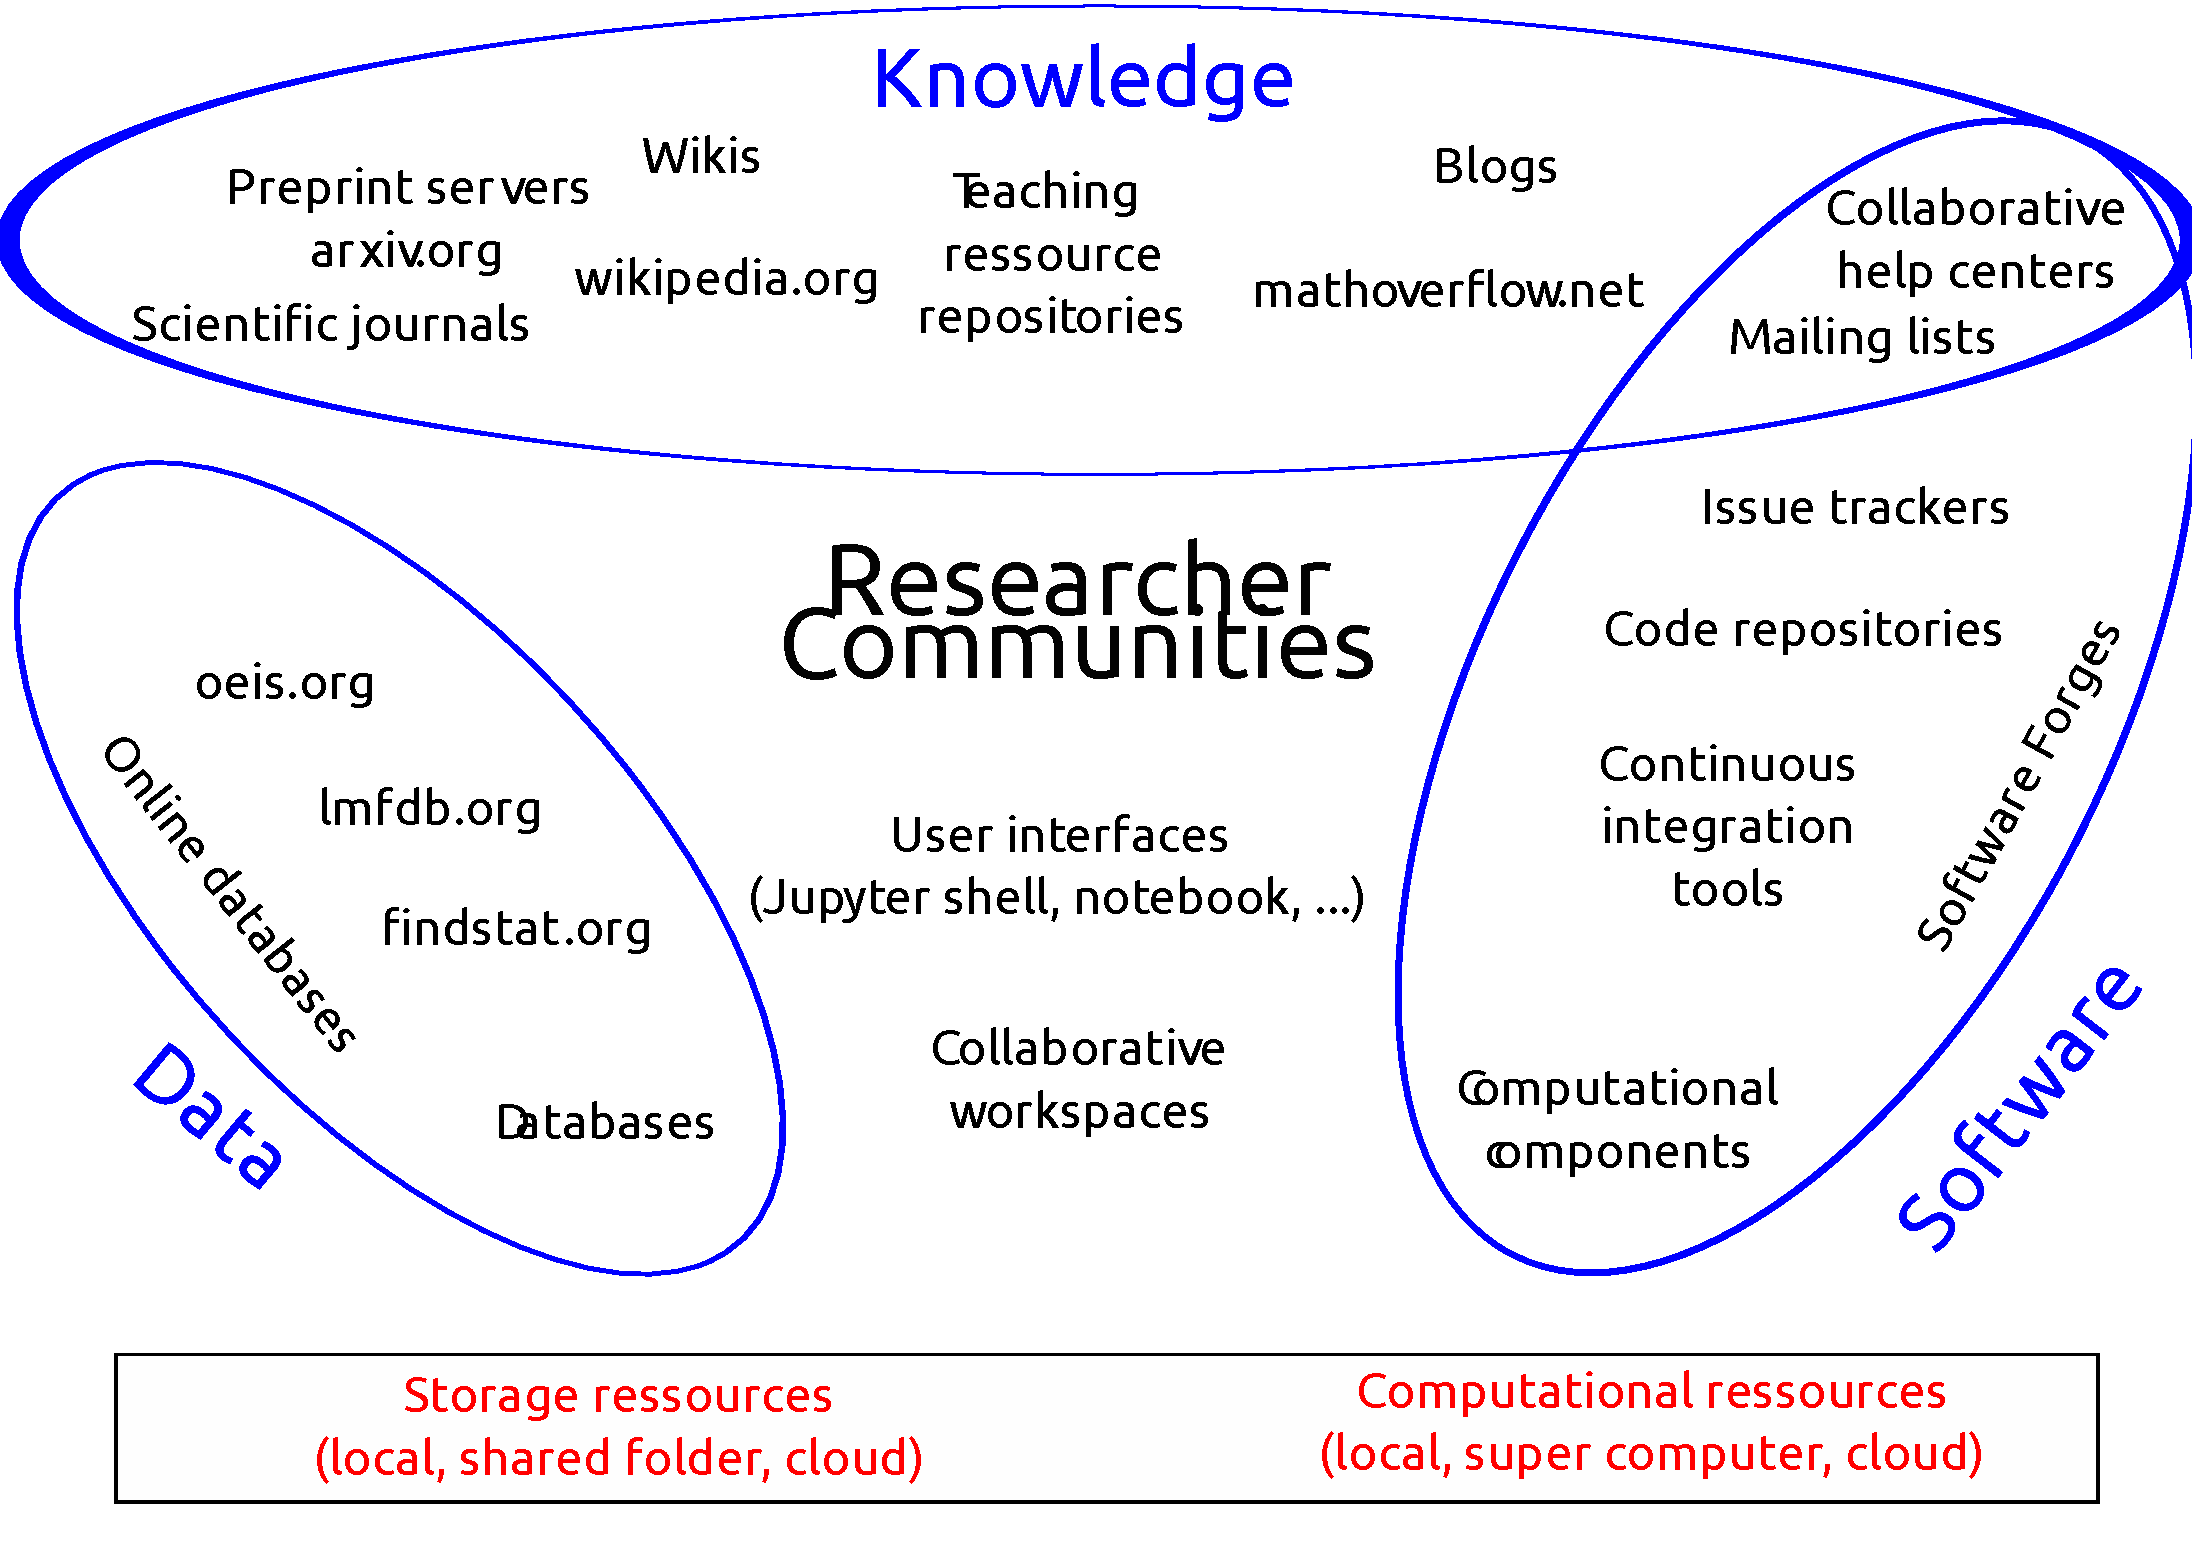
\includegraphics[width=\textwidth]{Pictures/TheBigPicture.pdf}}
  \caption{Virtual Research Environments for research in pure
    mathematics and applications.}
  \label{fig:thebigpicture}
\end{figure}

\TODO{ the findstat link does not work for me, kerning looks extremely weird -- POD}
\TODO{ both lmfdb and findstat have a strong knowledge component as well, with knowls and wikis}

\TODO{NT: the purpose of Figure~\ref{thebigpicture} is to give a quick
  sense of what Virtual Research Environments can be in our context,
  and a ``big picture'' for the project. A graphic artist friend of
  mine is going to help me improve it. I have collected here some material for her.\\\\
  \textbf{\Large What we would like the ``big picture'' in
    Figure~\ref{fig:thebigpicture} to highlight:}
  \begin{description}
  \item[This is a human centered project:] At the core: researchers and communities
    thereof.
  \item[The three types of information:]
    Software, Knowledge, Data (currently in blue)
  \item[Physical resources:]
    (currently in red)
  \item[Virtual Research Environments]\ 
    \begin{itemize}
    \item Researchers in Math have a long tradition of collaborating
      on Software, Knowledge, and, up to some point, Data
    \item For this they use a variety of collaborative tools which
      form a loosely knit Virtual Research Environment.
    \item \textbf{Aim 2}: make it easy for subcommunities of
      researchers to setup custom collaborative work spaces / Virtual
      Research Environments adapted to their needs, by combining:
      \begin{itemize}
      \item Computational resources
      \item Storage resources
      \item Computational software components
      \item Databases
      \item User interfaces
      \item Wikis-Knowledge bases (true for findstat, LMFDB): quicker
        cycle for consolidation of information spread over
        papers/brains
      \end{itemize}
      Such VRE shall help them:
      \begin{itemize}
      \item collaboratively develop software (e.g. specialized
        libraries), data and knowledge (e.g. articles) for their
        research projects.
      \item contribute back this information to the larger community
        whenever relevant.
      \end{itemize}
    \end{itemize}
  \item[Flow of information and processes:]\ \\
    It would be interesting to depict the following processes. They
    are indeed about collaboration and sharing (and quality control),
    that is what \textbf{Aim 1} is to promote.
    \begin{description}
    \item[Software development]\ 
      \begin{itemize}
      \item \emph{bug reports} and \emph{enhancement requests} emerge
        from the community, typically through collaborative help
        centers, and are posted on issue trackers.
      \item \emph{Design discussions} occur on mailing lists and issue
        trackers.
      \item Researchers \emph{submit code} to the code repositories.
      \item \emph{Quality control}: the code is reviewed and
        tested by continuous integration tools.
      \item Finally the code \emph{integrated} within computational
        components, and used by the community.
      \end{itemize}
      Researchers (as well as other users: teachers, engineers, ...)
      interact at each step of the process.
    \item[Production of data]\ \\
      Computational components $\Longrightarrow$ databases
    \item[Scientific publication]\ 
      \begin{itemize}
      \item researchers submit articles to journals and post them on
        preprint servers;
      \item the articles get reviewed by other researchers;
      \item finally they are distributed back to the community
      \end{itemize}
    \end{description}
  \end{description}
  %
  \textbf{\Large A collection of links that might give some idea of
    the look and feel of our universe:}
  \begin{description}
  \item[Examples of (computational) components:]\ 
    \begin{itemize}
    \item IPython: \url{http://ipython.org/}
    \item GAP: \url{http://www.gap-system.org/}
    \item Singular: \url{http://www.singular.uni-kl.de/}
    \item Sage: \url{http://sagemath.org/}
    \item Pari/GP: \url{http://pari.math.u-bordeaux.fr/}
    \item Linbox: \url{http://www.linalg.org/}
    \end{itemize}
  \item[Examples of online collaborative tools]\ 
    \begin{itemize}
    \item Issue tracker: \url{http://trac.sagemath.org/timeline/}
    \item Code repository: \url{https://github.com/}
    \item Collaborative help center: \url{http://ask.sagemath.org/}
    \item Collaborative math site: \url{http://mathoverflow.net/}
    \end{itemize}
  \item[Examples of online databases]\ 
    \begin{itemize}
    \item Online databases: \url{http://oeis.org/?language=french}
    \item LMFDB: \url{http://www.lmfdb.org/EllipticCurve/Q/14.a3}
    \item Findstat: \url{http://www.findstat.org/}
    \end{itemize}
  \item[Example of graphical material]\ 
    \begin{itemize}
    \item \url{http://boxen.math.washington.edu/home/nthiery/main2014.pdf}
    \end{itemize}
  \end{description}
}


\clearpage

\subsubsection{Why collaborative development of open source software?}

\TODO{Language to be moved in some form into the Concept section}

From their early days, computers have been used in pure mathematics,
either to prove theorems or, like the telescope for astronomers, to
explore new theories. Major achievements include the proof of the four
color theorem or \TODO{Nice flashy example?}. Usage has grown to the
point that certain areas of mathematics now completely depend on
experimental methods, with major efforts spent on software
development. As the sophistication of the required computations
increased, supported by the boom of the available computational power,
it became vital to share those efforts at the scale of large research
communities. European mathematicians have been pioneers and have grown
a steady tradition of collaborative open source software development,
with systems like GAP, Singular, or Pari/GP playing a major role for
decades.

\subsubsection{Importance of experimental tools in maths}

\TODO{Language to be moved in some form into the Concept section}

The field of computer algebra allows us to compute in and with a multitude
of mathematical structures. It is interdisciplinary in nature, with links to quite
a number of areas in mathematics, with applications in mathematics and other
branches of science and engineering, and with constantly new and often
surprising developments. Quite a number of these developments, in fact the
creation of whole subareas of the field,  have been iniated by European
researchers who made crucial contributions at all levels. These include the
design of fundamental algorithms, the development of major computer
algebra systems, applications of the computational methods in various fields,
and the creation of widely used databases.

Particular fruitful interactions unfold between computer algebra and
algebraic geometry, number theory, combinatorics and group theory. Algebraic algorithms
open up new ways of accessing subareas of these key disciplines of
mathematics, and they are fundamental to practical applications of the
disciplines. Conversely, challenges arising in algebraic geometry, number
theory, combinatorics and group theory quite often lead to algorithmic breakthroughs
which, in turn, open the door for new theoretical and practical applications
of computer algebra.

Based on exact computer aided calculations, the experimental method has
now been added to the toolbox of the pure mathematician. Experiments
lead to new conjectures which may have a deep impact on the future
development of mathematics. An outstanding example is the Birch and
Swinnerton-Dyer conjecture which is one of the Clay Millenium Problems.
Databases relying on computer calculations such as the Small Groups
Library or the Modular Atlas in group and representation theory provide
indispensible tools for researchers. A constructive way of understanding
proofs of deep theorems yields algorithmic tools to deal with highly abstract
concepts. These tools make the concepts available to a broader class of
researchers, with many potential applications. A prominent example from
algebraic geometry is the desingularization theorem of Hironaka, for which
Hironaka won the Fields Medal, and its algorithmization by Villamayor.

Spectacular theoretical breakthrougs such as Wiles' proof of Fermat's last
theorem are based on interdisciplinary approaches. Current developments
on the algorithmic side allow one to conquer crossconnections between
different areas of mathematics also computationally and, thus, to
arrive at cutting-edge applications which previously were inconceivable.

Other chunks of language:
\begin{itemize}
\item Mathematicians have a strong tradition of sharing knowledge
  openly (arxiv, Wikipedia, ...).

% Comment by William:
% > Regarding "Mathematicians have a strong tradition of sharing knowledge
% > openly", I think one reason for this is that the landscape of math
% > research is arguably *dramatically* larger than the research landscape
% > in any other field.  As a result, mathematicians find themselves in a
% > situation where collaboration is far more rewarding and productive
% > than competition, which results in a basic culture of sharing.  In
% > sharp contrast, in areas like drug discover or physics (or perhaps
% > even more intensely, in business!), being extremely competitive and
% > secretive is frequently the best strategy.  It is thus no surprise to
% > us that mathematicians are leading the way in developing tools for
% > collaboration and sharing.      Of course, many people outside of
% > mathematics simply don't know that there is anything to mathematics
% > "beyond calculus", so they don't realize how broad our research
% > landscape is.
% > 
% > I remember a professor in chemistry or physics coming to Sage Days 7
% > at IPAM (UCLA), and remarking that he was very surprised Sage was
% > coming from "number theorists", rather than computer science (say).  I
% > would imagine that computer science is also very competitive, since
% > it's a well-funded area with many people, but compared to mathematics
% > it's basically like one relatively small research area (within
% > combinatorics...).


\item Mathematicians have been building and sharing databases for a
  long while; the needs for such is growing tremendously, and the
  process needs to be streamlined.
\item Specific situation of maths w.r.t. Data:
  \begin{itemize}
  \item More often than not data is the result of a computation (and
    not e.g.  an experiment). The role of databases is thus primarily
    to store results for later reuse (persistent caching), and enable
    searches. Because of this, many issues (semantic, ontologies,
    reproducibility, ...) are to be treated upstream at the level of
    software rather than data.
  \item extreme reification in mathematics makes classical ontologies techniques/RDF impractical
  \item interlinking very high
  \item several alternate and defining description of same objects
  \end{itemize}
\end{itemize}

\draftpage

\subsection{Relation to the Work Programme}

\eucommentary{1-2 pages; Eugenia will help there}

\eucommentary{
Indicate the work programme topic to which your proposal relates, and
explain how your proposal addresses the specific challenge and scope
of that topic, as set out in the work programme.}

\eucommentary{
  \verbatiminput{call_description}
}

\draftpage

\subsection{Concept and Approach}
\eucommentary{5-8 pages}
\eucommentary{
-- Describe and explain the overall concept underpinning the project.
Describe the main ideas, models or assumptions involved. Identify
any trans-disciplinary considerations;
-- Describe and explain the overall approach and methodology, distinguishing, as
appropriate, activities indicated in the relevant section of the work programme, e.g.
Networking Activities, Service Activities and Joint Research Activities, as detailed in
the Part E of the Specific features for Research Infrastructures of the Horizon 2020
European Research Infrastructures (including e-Infrastructures) Work Programme 2014-
2015;\\
-- Describe how the Networking Activities will foster a culture of co-operation between the
participants and other relevant stakeholders.\\
-- Describe how the Service activities will offer access to state-of-the-art infrastructures,
high quality services, and will enable users to conduct excellent research.\\
-- Describe how the Joint Research Activities will contribute to quantitative and qualitative
improvements of the services provided by the infrastructures.\\
-- As per Part E of the Work Programme, where relevant, describe how the project will
share and use existing basic operations services (e.g. authorisation and accounting
systems, service registry, etc.) with other e-infrastructure providers and justify why such
services should be (re)developed if they already exist in other e-infrastructures. Describe
how the developed services will be discoverable on-line.\\
-- Where relevant, describe how sex and/or gender analysis is taken into account in the
project's content.}

\subsubsection{Linked research and innovation activities}

\eucommentary{Describe any national or international research and
  innovation activities which will be linked with the project,
  especially where the outputs from these will feed into the project;}

\TODO{For each item below, write a paragraph describing the project
  and one describing how it connects with this proposal}

\paragraph{DFG Priority Project SPP 1489}
\url{computeralgebra.de}

The SPP1489 ``Algorithmic and Experimental Methods in Algebra, Geometry, and
Number Theory'' is a nationwide Priority Project of the German Research Council DFG  
which commenced in July  2010 and will end in June 2016. The focus of the programme 
is on the interactions between computer algebra and algebraic geometry, number theory, 
and group theory. It combines expertise at all levels of research in computer algebra, 
be it the design of algorithms, the implementation of algorithms, the application
of algorithms, or the creation of mathematical databases. The goal of SPP1489 is to 
considerably further the algorithmic and experimental methods in the afore mentioned
disciplines, to combine the different methods across boundaries between the disciplines, 
and to apply them to central questions in theory and praxis. A fundamental concern of the
programme is the further development of open source
computer algebra systems with origins in Germany, which in
the framework of different projects will be crosslinked on
different levels. Of particular interest are interactions with application areas inside
and outside of mathematics such as system- and control theory, coding
theory, cryptography, CAD, algebraic combinatorics, and algebraic
statistics as well as hybrid methods which combine numerical and
symbolic approaches. 

\TOWRITE{WD}{One paragraph description of how this relates to this project}

\paragraph{IPython/Jupyter grant from the Alfred P. Sloan foundation}
\TOWRITE{IPython}{Proofread description of the Sloan grant and link to this project}

The IPython project received a \$1.15M grant from the Alfred P. Sloan
foundation that is supporting IPython development for two years
(1/1/2013-12/31/2014), in particular at the University of California,
Berkeley and California Polytechnic State University, San Luis Obispo.
This grant enabled the project to focus on developing the IPython
Notebook as a general tool for scientific and technical computing that
is open, collaborative and reproducible. This goes a long way toward
Aim \TODO{... and ...} of \TheProject, especially given the current
rapid evolution of IPython toward its language agnostic avatar
Jupyter.

\TheProject will build on the outcome of the Sloan grant, and further
develop the critical IPython/Jupyter component in close collaboration
with the IPython/Jupyter team. In particular, we plan to hire some of
the European developers that are currently funded by the Sloan grant
to work in California and wish to later return to Europe.

\paragraph{\SageCombinat grant}
\TOWRITE{NT}{...}

\paragraph{Logilab: simulagora, cubicweb, ...}

\TOWRITE{Logilab}{One paragraph description of simulagora, cubicweb, ...}
\TOWRITE{Logilab}{How does it relate to this project}

\paragraph{Sage Math Cloud}

\paragraph{FLINT grant?}

\paragraph{LMFDB grant}

The L-functions and Modular Forms Database (LMFDB) project originated
at a meeting at The American Institute for Mathematics (AIM) in 2007.
L-functions are ubiquitous in number theory, and have applications to
mathematical physics and cryptography. The simplest example of an
L-functions is the Riemann zeta function. Two of the seven Clay
Mathematics Million Dollar Millennium Problems deal with properties of
these functions, namely the Riemann Hypothesis and the Birch and
Swinnerton-Dyer Conjecture, that were conjectured following computational exploration.  
As well as providing a central repository
of data as a resource for researchers, through its website
\url{www.lmfdb.org}, the LMFDB provides a modern handbook, including
tables, formulas, links and references, concerning particular specific
L-functions and their sources.  Between 2008 and 2012 the LMFDB was
funded through a US National Science Foundation (NSF) Focussed
Research Grant (FRG) of around \$1M.  Since 2013, the funding of the
LMFDB has passed to Europe through a six year £2.2M Programme Grant
from the UK Engineering and Physical Sciences Research Council
(EPSRC), held at the universities of Warwick and Bristol, with
Professor John Cremona (Warwick) as its Principal Investigator (see
\url{http://www2.warwick.ac.uk/fac/sci/maths/people/staff/john_cremona/lmf}).
This grant supports six three-year postdoctoral research fellows,
mathematical researchers who work on the mathematical aspects of the
project full-time, biannual workshops, equipment and a portion of the
investigators' own time.

Almost all contributors to the LMFDB project, including those directly
supported by the EPSRC grant and the larger world-wide team of 30-50
contributors of data and code, are pure mathematicians.  Most of these
have good computational skills, but are not professional programmers
or software developers.  The LMFDB has a great need to broaden the
support it can call upon from software developers, to enhance the
project in several ways, including the computation of number-theoretic
data but more specifically in supporting the database management and
website user interface, in order to make the data more accessible and
useful to others.  The codebase of the LMFDB project is entirely open
source and hosted at github (https://github.com/LMFDB/lmfdb), written
in python with specialist modules such as flask and pymongo to manage
the website and database interface, and \Sage\ for higher-level
mathematical computations.  The LMFDB project would therefore benefit
greatly from collaboration with \TheProject as it would connect the
project with a pool of experts.  Joint workshops between the LMFDB and
\TheProject will stimulate and develop such collaboration: the LMFDB
places great importance on its workshops, which are small gatherings
of around 30 invited participants who work throughout one week on
certain specific aspects of the project, coming together in plenary
sessions to make decisions, plan and collectively approve of proposed
developments.  As a leading example of the use of databases in
mathematical research, the LMFDB will provide \TheProject\ with a real
large-scale prototype around which to develop new ideas about the
design and implementation of such databases and their associated
software.  The feasibility of such collaboration was successfully
tried at a workshop at the ICMS in Edinburgh in January 2013 on
``Online databases: from L-functions to combinatorics'', sponsored by
the NSF, AIM and the ICMS.

\paragraph{Findstat?}

\paragraph{Kwarc group}

\draftpage

\subsection{Ambition}

\eucommentary{1-2 pages}

\eucommentary{-- Describe the advance your proposal would provide beyond the
state-of-the-art, and the extent the proposed work is ambitious. Your answer
could refer to the ground-breaking nature of the objectives, concepts
involved, issues and problems to be addressed, and approaches and methods to be used.\\
-- Describe the innovation potential which the proposal represents. Where relevant, refer to
products and services already available, e.g. in existing e-Infrastructures.}

\draftpage

% ---------------------------------------------------------------------------
%  Section 2: Impact
% ---------------------------------------------------------------------------

\section{Impact}
\label{sec:impact}

\TODO{Orsay's grant services will help here in December}

\subsection{Expected Impacts}

\eucommentary{Please be specific, and provide only information that applies
to the proposal and its objectives. Wherever possible, use quantified
indicators and targets.\\
Describe how your project will contribute to:\\
-- the expected impacts set out in the work programme, under the relevant topic
(including key performance indicators/metrics for monitoring results and impacts);\\
-- improving innovation capacity and the integration of new knowledge
(strengthening the competitiveness and growth of companies by developing
innovations meeting the needs of European and global markets; and, where
relevant, by delivering such innovations to the markets;\\
-- any other environmental and socially important impacts (if not already
covered above).\\
Describe any barriers/obstacles, and any framework conditions (such as
regulation and standards), that may determine whether and to what extent
the expected impacts will be achieved. (This should not include any risk
factors concerning implementation, as covered in section 3.2.)}

\draftpage

\subsection{Measures to Maximise Impact}

\subsubsection{Dissemination and Exploitation of Results}
\label{subsubsect:dissemination}

\eucommentary{-- Provide a draft 'plan for the dissemination and exploitation
of the project's results'. The plan, which should be proportionate to the
scale of the project, should contain measures to be implemented both during
and after the project.\\
Dissemination and exploitation measures should address the full range
of potential users and uses including research, commercial, investment,
social, environmental, policy making, setting standards, skills and
educational training.\\
The approach to innovation should be as comprehensive as possible,
and must be tailored to the specific technical, market and organisational
issues to be addressed\\
-- Explain how the proposed measures will help to achieve the expected impact of the
project . Provide a draft business plan for financial sustainability as stated in the Part
E of the Specific features for Research Infrastructures of the Horizon 2020 European
Research Infrastructures (including e-Infrastructures) Work Programme 2014-2015.\\
-- Where relevant, include information on how the participants will
manage the research data generated and/or collected during the
project, in particular addressing the following issues:
What types of data will the project generate/collect? What
standards will be used? How will this data be exploited and/or
shared/made accessible for verification and re-use (If data cannot
be made available, explain why)? How will this data be curated and preserved?\\ \\
-- Include information about any open source software used or developed by the
project.\\
You will need an appropriate consortium agreement to manage (amongst other things)
the ownership and access to key knowledge (IPR, data etc.). Where relevant,
these will allow you, collectively and individually, to pursue market opportunities
arising from the project's results.\\
The appropriate structure of the consortium to support exploitation is addressed
in section 3.3. \\ \\
-- Outline the strategy for knowledge management and protection. Include measures to
provide open access (free on-line access, such as the ``green'' or ``gold'' model) to
peer-reviewed scientific publications which might result from the project.\\
Open access publishing (also called 'gold' open access) means that an article is
immediately provided in open access mode by the scientific publisher. The associated costs
are usually shifted away from readers, and instead (for example) to the university or
research institute to which the researcher is affiliated, or to the funding agency supporting
the research.\\
Self-archiving (also called ``green'' open access) means that the published article or the
final peer-reviewed manuscript is archived by the researcher - or a representative - in an
online repository before, after or alongside its publication. Access to this article is often -
but not necessarily - delayed (``embargo period''), as some scientific publishers may wish to
recoup their investment by selling subscriptions and charging pay-per-download/view fees
during an exclusivity period.}


\paragraph{Long term sustainability}

The success of large specialized software like \Pari, \Singular or
\GAP in the last decades has shown the viability of the academic open
source development model for such. For a long time, it was bitterly
debated whether this model would have any chance to scale to general
purpose systems for pure mathematics. The rapid take off of Sage in
the last 10 years has proven the viability of the ``developed by users
for users'' model: despite its large community of about 150 active
developers, it's running on a tiny specific budget, with most
activities being funded indirectly by research grants that require
specific development.

This was made possibly by reusing existing components whenever
possible (e.g. hundreds of specialized open source math libraries, or
the \Python programming language with its developers tools and huge
library), and spinning off software development (e.g. the \Cython
compiler) to larger communities whenever possible.

\TODO{This piece of argument is tricky to setup!!!}

Yet, long term critical non mathematical features like portability,
modularization, packaging, user interfaces, large data, parallelism,
or outreach toward related software, have been lagging behind. Indeed
they can hardly be implemented as a side product of research projects,
and \textbf{need to be assigned to full time developers}. Regular
funding is also needed to better structure the computational
mathematics community in Europe and support its upcoming major
widening through training, development workshops, exchanges, ...

The purpose of this grant is to initiate this process. The principle
is that, with the growth of the user base, a tiny number of
institutions or companies will hire a full-time developer because they
critically need it to support their in-house research or development.
\TODO{Examples: LRI? Full time devs supported by research grant, like
  for Linbox? Others?}

The number of such required full time developers will be made even
tinier because most of the efforts now will be focused toward
outsourcing or spinning off more components to reduce the recurrent
needs.

For example, this project will save much recurrent efforts to the
mathematics community by outsourcing the development of the user
interface to IPython. This grant will provide the required temporary
boost to make IPython stand to the stringent needs of the community.
Later on, thanks to its large user base, both in academia and
industry, IPython will continue to thrive without specific funding or
major contributions from the mathematics community.

Another big focus of this project will be on the study of open source
development models for mathematical software and how they can be made
more productive, in particular by better processes and collaboration
between components, which will also reduce the number of required full
time developers.

\draftpage

\subsubsection{Communication activities}
\label{subsubsect:communication}

\eucommentary{Describe the proposed communication measures for promoting the
project and its findings during the period of the grant. Where appropriate
these measures should include social media and public events with user
participation. Measures should be proportionate to the scale of the project,
with clear objectives. They should be tailored to the needs of various audiences,
including groups beyond the project's own community. Where relevant, include
measures for public/societal engagement on issues related to the project.}

\clearpage

% ---------------------------------------------------------------------------
%  Section 3: Implementation
% ---------------------------------------------------------------------------



\section{Implementation}

\TODO{Typical granularity: 5-8 work packages with 3-5 tasks and one
  deliverable per task; 10 milestones}

\subsection{Work Plan --- Work packages, deliverables and milestones}
\label{sect:workplan}

\eucommentary{Please provide the following:\\
\begin{itemize}
\item
brief presentation of the overall structure of the work plan;
\item
timing of the different work packages and their components (Gantt chart or similar);
\item
detailed work description, i.e.:
\begin{itemize}
\item
a description of each work package (table 3.1a);
\item
a list of work packages (table 3.1b);
\item
a list of major deliverables (table 3.1c);
\end{itemize}
\item
graphical presentation of the components showing how they inter-relate (Pert chart or similar).
\end{itemize}
}

\subsubsection*{Overall Structure of the Work Plan}

The work plan is broken down into XX workpackages as shown
in Figure~\ref{}: WP2 deals with  ...
In addition, there is one management work package (WP1) and one
general dissemination work package (\ref{m}). The Gantt chart on
Page~\pageref{fig:gantt} illustrates the timeline for the
various tasks for these work packages, including inter-task
dependencies.

%\newpage
\subsubsection*{How the Work Packages will Achieve the Project Objectives}
\label{sssec:how_the_work_packages_will_achieve}

\TOWRITE{ALL}{This needs to explain that we're actually going to meet the
objectives.  Needs to be done after objectives and WPs.}

The project objectives (Section~\ref{sect:objectives},
page~\pageref{sect:objectives}) and the corresponding work
packages that contribute to achieving those objectives are:

\begin{center}
\begin{tabular}{|l|l|l|}\hline
\textbf{Objective} & \textbf{Purpose} & \textbf{WPs} \\\hline \hline
Objective 1 & XX & \textbf{WPX} \\\hline
\end{tabular}
\end{center}

\paragraph*{Work Programme for Objective 1: }

Objective 1 is covered by WPX, which will ...

\landscape

\subsubsection*{Work Plan Timing: GANTT Chart showing Task Dependencies and Information Flows}


\vspace{-0.7in} \centerline{\hbox to \columnwidth{\hss%\includeimage[scale=0.85,angle=270]{ParaPhrase-Gantt2.pdf}
\hss}}
\label{fig:gantt}
\vspace{-1in} % Fool LaTeX into avoiding unnecessary page break
\endlandscape

\newpage

%\input{deliverables-dates}
%% Deliverables list.
%% Deliverables ordered by Workpackage
%% Workpackages are numbered automatically in sequence - the WP number has no effect

\workpackage{1}{Project Management}
\deliverable{mgt:mailinglists}
\deliverable{mgt:projectwebsite}
\deliverable{mgt:swrepository}
\deliverable{mgt:periodic-rep-1}
\deliverable{mgt:periodic-rep-2}
\deliverable{mgt:periodic-rep-3}
\deliverable{mgt:periodic-rep-4}
\deliverable{mgt:final-mgt-rep}

\workpackage{2}{}
\deliverable{del:xx}

\workpackage{3}{}
\deliverable{del:xx}

\workpackage{4}{}
\deliverable{del:xx}

\workpackage{5}{}
\deliverable{del:xx}

\workpackage{6}{}
\deliverable{del:xx}

\workpackage{7}{}
\deliverable{del:xx}

\workpackage{8}{}
\deliverable{del:xx}

\workpackage{9}{Dissemination, Exploitation and Communication}
\deliverable{del:pressrelease} % Press release.
\deliverable{del:website} % Project presentation (web site). 
\deliverable{del:workshop1}  % Report on first project workshop, year 1. 
\deliverable{del:dissemplan1} % Final plan for using and disseminating knowledge.
\deliverable{del:workshop2}  % Report on second project workshop, year 2
\deliverable{del:workshop3}  % Report on third project workshop, year 3
\deliverable{del:dissemplan2} % Final plan for using and disseminating knowledge.



\addtocounter{subsubsection}{1}
\addcontentsline{toc}{subsubsection}{\protect\numberline{\thesubsubsection}Work
Package List}
\fbox{\begin{minipage}{\textwidth}\begin{center}{\Large\bf
        Work package list} % (full duration of project)}
  \end{center}
  \end{minipage}}

\bigskip\bigskip

\begin{tabular}{|p{1.2cm}|p{9.15cm}|p{0.8cm}|p{1.2cm}|p{1cm}|p{0.9cm}|p{0.9cm}|}
\hline
{\bf Work \mbox{package} No} & {\bf Work package title} &
{\bf Lead \mbox{partic.} no.} &
{\bf Lead short name} &
{\bf Person months} & {\bf Start month} & {\bf End month} \\\hline

\newcounter{wp}

% 1 Management
\addtocounter{wp}{1}
\workpackageentry{\thewp}{PS}{}{1}{60}

% 2 Community building and engagement
\addtocounter{wp}{1}
\workpackageentry{\thewp}{PS}{}{}{}

% 3 Component architecture
\addtocounter{wp}{1}
\workpackageentry{\thewp}{PS}{}{}{}

% 4 User interfaces
\addtocounter{wp}{1}
\workpackageentry{\thewp}{PS}{}{}{}

% 5 HPC and massively parallel computation
\addtocounter{wp}{1}
\workpackageentry{\thewp}{PS}{}{}{}

% 6 Next generation databases
\addtocounter{wp}{1}
\workpackageentry{\thewp}{SA}{}{}{}

% 7 Development models
\addtocounter{wp}{1}
\workpackageentry{\thewp}{}{}{}{}

% 8 Social aspects
\addtocounter{wp}{1}
\workpackageentry{\thewp}{UO}{}{}{}

% 8 Dissemination
\addtocounter{wp}{1}
\workpackageentry{\thewp}{SA}{}{}{}

{\textbf{Total}} & & & &
\textbf{\large XXX}&
&
\\\hline
\end{tabular}


% \textbf{Summary:}\\[1ex]

\newpage

\fbox{\begin{minipage}{\textwidth}\begin{center}\Large\bf List of Deliverables
  \end{center}
  \end{minipage}}

\label{sect:deliverables}

\bigskip\bigskip\bigskip

\begin{minipage}{\textwidth}
\begin{center}
\begin{tabular}{|p{0.8cm}|p{8.75cm}|p{0.8cm}|p{1.2cm}|p{1.2cm}|p{1.2cm}|p{1.2cm}|}  \hline
\textbf{Del. no.}              & \textbf{Deliverable name}        & \textbf{WP no.} & \textbf{Lead}
& \textbf{Type}              & \textbf{Dissemi- nation level}   & \textbf{Delivery date}
\\ \hline

%% Year 1

%\ref{del:xx}  & Requirements Analysis
%& WP? & & R & CO &  ?? \\
\hline
\end{tabular}
\end{center}
\end{minipage}


\newpage

%% Set up the milestone numbers.

The work in the \TheProject project is structured by four milestones,
which coincide with the four project meetings held at the end of each
year of the project (the other four meetings will be held in the middle
of each year). Given the nature of the project, with a
large number of essentially independent tasks, there is no need for
milestones attached to specific collections of tasks or
deliverables. Instead, given that the meetings are the main
face-to-face interaction points in the project, it's suitable to
schedule the milestones for these events, where they can be discussed
in detail, tracking the progress in each work package through status
reports on the tasks and deliverables.

We envisage that this setup will give the project the vital coherence
in spite of the broad interdisciplinary mix of various backgrounds of the
participants.

% \newcommand{\WPall}{\WPref{management}, \WPref{dissem}, \WPref{component-architecture}, \WPref{UI}, \WPref{hpc}, \WPref{dksbases}, \WPref{social-aspects}}

% \newcommand{\WPnoUI}{\WPref{management}, \WPref{dissem}, \WPref{component-architecture}, \WPref{hpc}, \WPref{dksbases}, \WPref{social-aspects}}

% \begin{center}
%   \begin{tabular}{|m{.05\textwidth}|m{.30\textwidth}|m{.15\textwidth}|m{.05\textwidth}|m{.22\textwidth}|}
%     \hline
%     Mile-stone nr. & Milestone name & Related work packages & Est. date & Means of verification \\\hline
%     M1 & Requirements study, design and prototype implementations. Start of
%          community building.
%        & \WPall 
%        & 12 
%        & 2nd Project meeting report. Completion of corresponding deliverables. \\\hline
%     M2 & First fully functional interface implementations.
%          Enhanced versions of \TheProject components.
%          Training early adopters.
%        & \WPall 
%        & 24 
%        & 4th Project meeting report. Completion of corresponding deliverables. \\\hline
%     M3 & Evaluating \TheProject software. Working with the community 
%          and building portfolio of experiments produced with \TheProject.
%        & \WPall 
%        & 36 
%        & 6th Project meeting report. Completion of corresponding deliverables. \\\hline
%     M4 & Project evaluation and final versions of all \TheProject components.
%        & \WPnoUI 
%        & 48 
%        & 8th Project meeting report. Completion of corresponding deliverables. \\\hline
%   \end{tabular}
% \end{center}

\begin{milestones}
  \milestone[id=startup,month=12,
  verif={Completed all corresponding deliverables and reported the progress in the 2nd Project meeting report.}]
  {Startup}
  {By Milestone 1 we will have carried out the requirements study, design and prototype implementations and started community building activities.}

  \milestone[id=proto1,month=24,
  verif={Completed all corresponding deliverables and reported the progress in the 4th Project meeting report.}]
  {Prototypes}
  {By Milestone 2 we will have constructed first fully functional interface implementations and released enhanced versions of \TheProject components, and train early adopters of \TheProject.}

  \milestone[id=community,month=36,
  verif={Completed all corresponding deliverables and reported the progress in the 6th Project meeting report.}]
  {Community/ Experiments}
  {By Milestone 3 we will have gathered and evaluated feedback on \TheProject software and established the portfolio of experiments produced with \TheProject through further engaging with the community.}

  \milestone[id=eval,month=48,
  verif={Completed all corresponding deliverables and reported the progress in the 8th Project meeting report.}]
  {Evaluation}
  {By Milestone 4 we will have released final versions of all \TheProject components and completed the project evaluation.}
\end{milestones}

%%% Local Variables:
%%% mode: latex
%%% TeX-master: "proposal"
%%% End:

%  LocalWords:  verif ldots


\fbox{\begin{minipage}{\textwidth}\begin{center}\Large\bf List of milestones
  \end{center}
  \end{minipage}}
\label{sect:milestones}

\bigskip\bigskip\bigskip

\begin{minipage}{\textwidth}
\begin{center}
\begin{tabular*}{\textwidth}{|p{1.5cm}|p{6.7cm}|p{2.5cm}|p{1.5cm}|p{3.6cm}|}  \hline
\textbf{Milestone number} & \textbf{Milestone name} & \textbf{Related work
  package(s)} & \textbf{Estimated date} & \textbf{Means of
  verification} (deliverables shown here + success criteria below) \\
\hline
\ref{mil:initial} &
  Completed initial requirements analysis.  &
  WPX &
  1 &
\ref{del:requirements-analysis}.
\\
\ref{mil:final} &
&
WPX &
&
\\
\hline
\end{tabular*}
\end{center}
\end{minipage}

\vspace{10pt}
\begin{center}
\begin{tabular*}{\textwidth}{|p{1.5cm}|p{13.3cm}|p{1.9cm}|}\hline
\textbf{Milestone} & \textbf{Success Criteria} & \textbf{Contributes to
  Objective(s)} \\\hline
\ref{mil:initial} &
Completed requirements analysis (Deliverable~\ref{del:requirements-analysis}). &
 \textbf{1, 3.}
\\
\ref{mil:final} &
XX
& \textbf{XX}
\\\hline
\end{tabular*}
\end{center}

\eucommentary{
KEY
Estimated date
Measured in months from the project start date (month 1)
Means of verification
Show how you will confirm that the milestone has been attained. Refer to indicators if appropriate.
For example: a laboratory prototype that is ‘up and running’; software released and validated by a
user group; field survey complete and data quality validated.
}

% ---------------------------------------------------------------------------
% Include Workpackage descriptions
% ---------------------------------------------------------------------------

\newpage
\subsection{Work Package Descriptions}\label{sec:workpackages}
%% WP titles and order are defined in deliverables.tex
%%% work package style may be broken -- fix this!!

%% Local WP number counter - should possibly be global and hidden?
\begin{workplan}
\begin{draft}
\TOWRITE{PS (Work Package Lead)}{For WP leaders, please check the following (remove items
once completed)}
\begin{verbatim}
- [ ] have all the tasks in this Work Package a lead institution?
- [ ] have all deliverables in the WP a lead institution?
\end{verbatim}
\end{draft}



\begin{workpackage}[id=management,type=MGT,wphases=0-48!.2,swsites,
  title=Project Management,short=Management,
  lead=PS,
  PSRM=28,SARM=2,  
  USORM=2,LLRM=2,UVRM=2,UJFRM=2,UBRM=2,UORM=2, USHRM=2, USORM=2,
  UWRM=2, JURM=2, UKRM=2, USRM=2, ZHRM=2, SRRM=2, UWSRM=2]

\begin{wpobjectives}
%  The objectives of this work package are to undertake all project management activities,
%  including:
%  \begin{compactitem}
%  \item monitoring the overall progress of the project and the use of
%    resources;
%  \item ensuring the timely production of deliverables and other
%    project outputs;
%  \item reporting to the European Commission on financial matters;
%  \item preparing for and attending the annual project review
%    meetings; and
%  \item managing the project Advisory Board.
%  \end{compactitem}

Establish and maintain an effective contract, project, and operational management
approach, ensuring (i) an effective and timely implementation of the project, (ii) quality control
of the results, (iii) risk and innovation management of the project as a whole, as well as (iv)
timely and necessary interaction with the EC and other interested parties.

  % The objective of  is to undertake all project management
  % activities, including setting up joint infrastructure, organizing
  % meetings, and producing overview reports.
\end{wpobjectives}

\begin{wpdescription}
The project will be managed by UPS, which has profound experience in administrating and leading EU funded and national projects. The coordinator together with the WP leaders, will be responsible for monitoring WP status, coordination of work plan updates and annual internal progress reports. The project management structure  and roles of partners in the consortium are presented in the next section.
\end{wpdescription}

\begin{tasklist}
\begin{task}[title=Project and financial management,
id=project-finance-management,lead=PS,PM=33]
The task includes the following activities
  \begin{compactitem}
\item Preparation and Distribution of the Consortium Agreement;
\item Setup project website, intranet and communication procedures for effective communication;
\item Organization of project review and progress meetings;
\item Establishment and maintenance of external contacts (with the EC, 
other relevant national / EU projects, other academic and industrial stakeholders) to organize transfer of knowledge, present and
promote project results;
\item Progress and Financial Reporting to the EC;
\item Data and IPR Management will be managed in accordance with agreed rules stated in the
Consortium Agreement and in accordance with the Data management plan (Task X.Y).
  \end{compactitem}
\end{task}

\begin{task}[title=Quality assurance and risk management,
id=project-finance-management,lead=PS,PM=15]
A quality assurance plan will be established to ensure coherent and sufficient quality of the work
and results. The plan will be developed by UPS, involving all partners, and will be followed up
regularly. In addition, the partners will establish and follow regularly a risk management plan
and self-assessment to ensure that technical barriers / potential risks are identified  and corrective measures are put into place on time.
\end{task}

\begin{task}[title=Innovation management,
id=project-finance-management,lead=PS,PM=10]

One of the most important criteria for success for the OpenDreamKit project is to bring the project results into use. Therefore, exploitation routes will be sought whenever possible. In
order to create a common understanding within the Consortium about how we can best usher
an idea all the way from conception to its realization and exploitation, the Coordinator will be responsible for
the preparation and realization of an Innovation Plan to assure that research activities meet the
required milestones and the outputs of innovation are fully aligned with the project objectives.
All research activities will go through three initial steps where the exploitation opportunity is
identified along with the main stakeholders for the exploitation opportunity and an IP owner.
\end{task}
\end{tasklist}

%
%  This workpackage will perform all the activities related to monitoring of progress
%  towards the project milestones shown on Page~\pageref{sec:milestones} and the
%  deliverables listed on Page~\pageref{sec:deliverables}, assuring the quality of the
%  deliverables, ensuring the collation and distribution of the required reports,
%  questionnaires and deliverables including the annual reports to the European Commission,
%  arranging project management meetings, tracking the project budget in terms of
%  expenditure and person-months, obtaining financial certificates as required, convening
%  project management meetings, ensuring that important project documents such as the
%  project contract and the consortium agreement are properly maintained and amended as
%  necessary, ensuring that contractual details are complied with, monitoring compliance
%  with the grant agreement, preparing for the annual review meetings, and reviewing
%  research results against the aims and objectives of the project. It also involves
%  managing and supporting the project Advisory Board, including supporting attendance at
%  project meetings, convening Advisory Board meetings, and obtaining feedback on the
%  project direction and results.


\begin{wpdelivs}
\begin{wpdeliv}[due=1,id=ca,dissem=CO,nature=R]{Consortium Agreement}
\end{wpdeliv}

\begin{wpdeliv}[due=1,id=tickets,dissem=PU,nature=DEC]{Establishing basic project infrastructure 
    (websites, wikis, issue trackers, mailing lists, repositories)}
\end{wpdeliv}

\begin{wpdeliv}[due=12, 36,id=ipr,dissem=CO,nature=R]{Internal Progress Reports, including risk management and quality assurance plan}
\end{wpdeliv}

\begin{wpdeliv}[due=18, 45,id=tickets,dissem=CO,nature=R]{Innovation Management Plan}
\end{wpdeliv}


%\begin{wpdeliv}[due=12,id=periodic-rep-1,dissem=PU,nature=OTHER]{First Annual Report (first year)}
% \end{wpdeliv}
%\begin{wpdeliv}[due=24,id=periodic-rep-2,dissem=PU,nature=OTHER]{Project Annual Report (second year)}
% \end{wpdeliv}
%\begin{wpdeliv}[due=36,id=periodic-rep-3,dissem=PU,nature=OTHER]{Project Annual Report (third year)}
% \end{wpdeliv}
%\begin{wpdeliv}[due=48,id=periodic-rep-4,dissem=PU,nature=OTHER]{Project Annual Report (fourth year)}
% \end{wpdeliv}
%\begin{wpdeliv}[due=48,id=final-mgt-rep,dissem=PU,nature=OTHER]{Project Final Report}
% \end{wpdeliv}
\end{wpdelivs}
\end{workpackage}
%%% Local Variables: 
%%% mode: latex
%%% TeX-master: "../proposal"
%%% End: 

%  LocalWords:  workpackage wphases wpobjectives wpdescription pageref wpdelivs wpdeliv
%  LocalWords:  dissem mailinglists swrepository final-mgt-rep compactitem swsites
\newpage
\begin{draft}
\TOWRITE{VP (Work Package Lead)}{For WP leaders, please check the following (remove items
once completed)}
\begin{verbatim}
- [ ] have all the tasks in this Work Package a lead institution?
- [ ] have all deliverables in the WP a lead institution?
- [ ] do all tasks list all sites involved in them?
- [ ] does the table of sites and their PM efforts match lists of sites for each task?
      (each site from the table is listed in all relevant tasks, and no site is listed
      only in the table or only at some task)
\end{verbatim}
\end{draft}



\begin{workpackage}[id=dissem,wphases=18-48!.5,
  short={Community Building/Dissemination},
  title={Community Building, Training, Dissemination, Exploitation, and Outreach},
  lead=PS,
  PSRM=15,
  SARM=18,
  USORM=10,
  USHRM=8,
  USRM=24,
  UVRM=2,
  UBRM=20,
  SRRM=2
]


\begin{wpobjectives}
  The objective of this work package is to further develop the community at the
  European scale, foster cross teams collaborations, spread the
  expertise, and engage the greater community to participate to the
  definition of the needs, and the implementation and use of the
  produced solutions. This includes:

  \begin{compactitem}
  \item reviewing emerging technologies;
  \item ensuring awareness of the results in the user community;
  \item engaging cross communities discussions to foster scientific collaborations and conjoint developments;
  \item spreading the expertise through workshops and trainings;
  \item defining individual exploitation plans; and,
  \item managing existing and new intellectual property.
  \end{compactitem}
\end{wpobjectives}

\begin{wpdescription}
  We will organize regular open workshops (e.g. Sage Days, Pari Days,
  summer schools, etc.); some of them will be focused on development
  and coding sprints, and others on training. This is also an occasion
  to organize cross communities workshops like Sage-Jupyter days.

  This work package will also provide general travel budget to fund
  short to long term visits between the participants, to collaborate
  on specific features. A typical such visit would bring together an
  IPython developer with a GAP developer for a couple of days to
  implement a first prototype of notebook interface to GAP.

  We will also make all code, documents, test and build infrastructure
  for the micromagnetic simulator available, and deliver a number of
  workshops to the relevant community to disseminate this, and exploit
  feedback and contributions from them.

  This work package will complement and lean on a parallel COST
  network whose role is to build and animate the greater community.
\end{wpdescription}

\begin{tasklist}
\begin{task}[title=Reviewing emerging technologies, id=tech-review]
  In this task, we will produce periodic reviews of emerging
  technologies and relevant developments elsewhere, and implications
  for our plans. This include the review of standard components and
  service for storage and sharing, computational resources,
  authentication, package management, etc. This may further include
  negotiating access or shared development when appropriate. This
  information will be fed to the other work packages, in particular
  Work Package~\WPref{component-architecture} Component Architecture.
\end{task}

\begin{task}[title=Dissemination and Communication activities, id=dissemination-communication]

  \TOWRITE{VP}{scale this down as appropriate}

  This task comprises all forms of direct dissemination and public
  communication activities such as press releases, creation of the
  project web-site including visitor analysis and monitoring tools,
  scientific and technical publications, outreach activities
  (seminars, keynote talks, media interviews, press releases),
  pro-motion through social media (e.g. Twitter, Facebook, LinkedIn),
  creation of advertisement materials such as flyers, posters, and
  electronic feeds as well as their distribution.

  % News articles will be produced by experienced professional staff
  % at relevant partners including ... and communicated to local,
  % national and international media, as appropriate.

  At least two press releases will be generated in the course of the
  project.
  \TOWRITE{VP}{Neil: this coming year i will do four workshops, although the
    number may be smaller by the time we are up and running. an
    additional component that could be integrated here is a 'JMLR
    Monthly Notices' section that I recently gained approval for. This
    is a new section the leading machine learning journal that we'll
    aim to focus on typically smaller advances (less than a full
    paper). A little like a 'Nature Notices' section but much more
    informal and open. We don't yet know the best way of doing it, but
    the mechanism might be similar to ways we'd want to disseminate
    \TheProject results.}
\end{task}

\begin{task}[title=Community building: development workshops, lead=PS, partners={UB}, id=devel-workshops]

We will organize development workshops all throughout the project. The
aim of these workshops is to bring together developers from the
different communities to implement some key aspects of \TheProject:
user interface, documentation, cross compatibility, etc. These
meetings will gather not only participants of \TheProject but also
members of the different communities involved. Bringing talented
people together is the best way to make actual progress on the
different aspects of \TheProject. It is also a way to work within the
communities we're reaching and include them in the discussions and
development. It fosters collaborations between scientists and
developers from different backgrounds to build tools that are needed
by all.

Each workshop will be aimed at a specific software (\Sage, \GAP, \SMC,
\IPython, \Singular, etc.) or be joint meeting between different
communities to improve interoperability and joint developments. We are
planning to have 4 or 5 such events per year and will produce a
activity report every year. More precisely, here is a tentative list
of the different events planned so far:

\begin{compactitem}
\item One \Sage worshop per year in Cernay France (near Orsay) where
  similar gatherings took place before. One of them will be a
  Sage-Sphinx day, dedicated to documentation.

\item One Atelier \Pari in Bordeaux per year. The team in Bordeaux has
  a great experience in organizing this kind of \Pari events.

\item Two \Singular workshops and two \GAP workshops in Kaiserslautern
  over the four years.

\item Two workshops dedicated to high performance mathematical
  computing in relations with \WPref{hpc}. One of them should be in
  Grenoble and the second one in Bordeaux to foster the work with
  \Pari towards \taskref{hpc}{hpc-pari}.

\item A joint meeting on the topics of \SMC and \Jupyter in Simula in
  relations with \WPref{UI}.

\item A joint event between \GAP, \Sage, and \Singular in ICMS,
  Edinburgh.

\item A joint \Jupyter and \Sage event in Orsay.

\item A joint \LMFDB and \Sage event in Warwick to work towards
  \WPref{dksbases}.

\end{compactitem}

\TOWRITE{VP}{Add workshop report to the deliverables}

\end{task}

\begin{task}[title=Dissemination: reaching users, lead=PS, partners={UB}, id=dissemination]

As lead developers of \TheProject, most of us consider themselves as both scientists and developers.
And we have experience into reducing the gap between those two worlds. We organize trainings, workshops such as Sage-days to promote our tools and bring more users and developers from the scientific world. On the other hand, we're often present to more development-oriented gatherings like PyCon and SciPy to exchange with engineers and foster collaborations.

The aim of this task is to keep this winning strategy on within \TheProject. Three events should be organized in the spirit of Sage-days to gather and train more users and foster scientific development around \TheProject. These conferences usually welcome around 50 participants and have a big impact on the scientific community. One of them will be at CIRM in Marseille, another one at ICMS in Edinburgh and a third one probably in Dagstuhl Germany. In the same spirit, we will also have training sessions organized within the universities (Orsay and Grenoble). We will also run a series of 4 workshops in developing countries especially Africa and South America. Some of these workshops will be joined to CIMPA schools (\delivref{dissem}{developing-countries1}, \delivref{dissem}{developing-countries2}, \delivref{dissem}{developing-countries3}, \delivref{dissem}{developing-countries4}).
The CIMPA is an international organization based in Nice (France) that promote
research in mathematics in developing countries. It organizes each year around
20 schools.

The under-representation of women in the scientific world is even more perceptible when we intersect science with software development. As we know we have many talented women in our community, we will organize some events targeted at women in the spirit of the "Women in Sage" days that happened many times in the US already. We are planing to have two of them in Orsay and at least one in Oxford where some "Women in CS" days already took place.

Apart from this different events, we will also be present at important events of both our scientific community (international mathematical conferences such as FPSAC for combinatorics) and the python / open-source software development community: PyCon, SciPy, EuroPython, etc.


\end{task}


%Mike Croucher and Neil Lawrence,Sheffield
\begin{task}[title=Introduce \TheProject to researchers and teachers, id=project-intro,lead=USH,PM=6]

In this task, we will develop and deliver materials that will
introduce \TheProject to potential users---both researchers and
teachers.

Develop a `taster' seminar (1-2 hours) and follow-up short course (1-2
days) on \TheProject for researchers and lecturers in all disciplines
\delivref{dissem}{short-course}. At Sheffield, this will be added to
the set of courses that are offered as part of IT Services' research
support department. As such, it could potentially reach all
disciplines. It will also be made publicly available for widespread
dissemination and collaborative modification.

Elements of this work will also be integrated with the GP Summer
Schools and Roadshows. The Summer School is now in its fourth edition
(over 140 students educated). The Roadshows have taken place in
Uganda, Colombia and are scheduled for Italy, Australia and Kenya.

These seminars and short-courses will be used to identify potential
collaborators who are interested in utilising \TheProject
immediately. We will act as consultants to these collaborators in two
ways:

We will work with lecturers at Sheffield to introduce \TheProject to
various disciplines via the production of interactive lecture
notes \delivref{dissem}{lecture-notes}. The focus for the student here will not necessarily be on
programming but rather on interaction with the subject matter via use
of \TheProject. Interactive lecture notes are an area where commercial
vendors such as MapleSoft and Wolfram Research are spending a lot of
time and money developing material. We will provide technical and
programming expertise to lecturers---helping them to develop the
interactive part of notes while they provide the subject material.

We will work as consultants with researchers at Sheffield to introduce
\TheProject to their workflow. Any projects that successfully do this
will be promoted as case studies for \TheProject.
\end{task}

\begin{task}[id=dissemination-of-oommf-nb-virtual-environment,
  title=Open source dissemination of micromagnetic VRE,
  lead=USO,PM=4,partners={SR,USH,PS}]
  % 3 months person time + 1 months investigator time
  Tasks \taskref{UI}{oommf-py-ipython-attributes} and
  \taskref{UI}{oommf-tutorial-and-documentation} provide the
  micromagnetic VRE demonstrator
  (\ref{sec:introduction-micromagnetic-vre-demonstrator}) built on top
  of \TheProject.  In this task, we set up of the infrastructure
  (\delivref{dissem}{oommfnb-source-and-testing-setup}) to encourage
  and invite code contributions from the micromagnetic community to
  both code and created notebooks, while automating quality control
  and maintaining trust effectively.

  The source code of the micromagnetic VRE will be made available as
  open source on public repository hosting sites (such as
  GitHub/Bitbucket), and announced to the community via appropriate
  mailing lists and other means. We will set up a publicly accessible
  Jenkins/Travis continuous integration (CI) system to (i) run
  regression tests (from
  \taskref{component-architecture}{oommf-python-interface} and
  \taskref{UI}{oommf-py-ipython-attributes}) routinely when the
  micromagnetic VRE code or underlying OOMMF core code changes, (ii)
  re-execute notebooks (from
  \taskref{UI}{oommf-tutorial-and-documentation}) and use them as
  regression tests (using the outcome of task
  \taskref{UI}{notebook-verification}), and (iii) re-build
  downloadable installation files and virtual machine images.
  %This set
  %up will test user-contributions automatically.

  %versions (\delivref{dissem}{oommfnb-source-and-testing-setup}).

\end{task}

\begin{task}[title=Micromagnetic VRE dissemination workshops,
id=dissemination-of-oommf-nb-workshops,lead=USO,PM=6]

  % 3 months person time, 2 months investigator time

We will run a series of workshops
(\delivref{dissem}{oommfnb-workshops}) during the evenings of 4 major
international meetings on magnetism research\footnote{Anticipated most
  significant international meetings in the appropriate time frame are
  61st Conference on Magnetism and Magnetic Materials (MMM2016), October
  31-November 4, 2016, New Orleans, Louisiana; 62nd Conference on
  Magnetism and Magnetic Materials (MMM 2017), November 6-10, 2017, Pittsburgh,
  Pennsylvania; 21st International Conference on Magnetism (ICM 2018),
  July 16–20, 2018, San Francisco, California; 14th Joint MMM-Intermag
  Conference (MMM2019), January 14-18, 2019, Washington, DC). Each of those
  meetings is one week long, and serves as a focal point of networking
  for the european and international research community. Other training events have been held in the
past at these conferences and were well attended.} to
disseminate the micromagnetic virtual research environment
(Sect. \ref{sec:introduction-micromagnetic-vre-demonstrator} and  
\localtaskref{dissemination-of-oommf-nb-virtual-environment}) in the
micromagnetic community. Each conference
attracts around 1500 participants, and we expect at least 30 for our
workshops at every event. Depending on demand, multiple workshops
will be given per conference.

The taught material will include (i) use of the \Jupyter-based
micromagnetic VRE, and an (ii) introduction to the standard techniques
for contributing to open source software (version control, pull
requests, testing frameworks) to foster excellence in computational
science and to make the micromagnetic VRE project self-sustaining as quickly
as possible. In addition, all teaching materials, including videos,
will be made available on a website.

For each workshop, we request \euro{500} room hire at the magnetism conference
location and the travel expenses for two teachers from Southampton to
attend the one week international conference, totalling (\euro{500} +
2x\euro{2200}=\euro{4900}) per workshop. There are no other costs.
\end{task}

\begin{task}[title=Demonstrator: Interactive books,
id=ibook,lead=US,PM=30]
  % 2x12 _ 3x 3 months for students

One of the important elements of VREs is a common flexible writing format which
enables the creation of large structured documents. There are many
known solutions to that problem, but they usually compromise the
interactivity of the notebook interface and typesetting quality of desktop
publishing software like LaTeX.

Recently, a few approaches tried to bring both interactivity and the
typographic features. The modestly tagged markup language
\href{http://hplgit.github.io/doconce/doc/web/}{DocOnce}
targets the problem of reusability of the document source code for
producing traditional LaTeX-based printed books, IPython notebooks, Sphinx
documents (with Sage cells), and many other formats. MathBook XML
is a lightweight XML application for authors of scientific articles,
textbooks and monographs extensively using Sage cells for
interactive elements. The Sphinx documentation software has been
successfully applied for creation of interactive books containing Sage
cells. Additional interactivity is offered using the \href{http://runestoneinteractive.org}{Runestone tools}.

The technical aspects of format for interactive publications is a
subject of the task ``Structured documents'' in
\taskref{UI}{structdocs}. In this task we will demonstrate usability
of the results of \taskref{UI}{structdocs} in creation of scientific
textbooks. Three interactive books will be created:

\begin{compactitem}
\item Nonlinear Processes in Biology
\item Classical and Quantum Mechanics
\item Problems in Physics with Sage/Python
\end{compactitem}

The choice of those particular topics has been made for the sake of
maximal diversity. The ``Nonlinear Processes in Biology'' will heavily
use numerical solution of ODEs and PDEs.
Classical and Quantum Mechanics will demonstrate power of
CAS systems working ``on par'' with numerical tools. The last example
will focus mostly on collaborative editing and modularity of content
which is produced using VRE technologies.

The main research aspect for this task will be to integrate modern
computational tools in classical scientific topics and explore how
the VRE environment can accelerate the development and produce electronic
documents with significantly enhanced pedagogy.

In particular we will answer following questions:

\begin{compactitem}
\item When is a fully interactive worksheet required and when is
  a textbook with executable code cells sufficient?
\item How to assemble a classical monograph by reusing independently working
  building block of text and code?
\item What are best tools and practices for using a single source for
  producing printed and electronic (interactive) textbooks?
\item How to collaboratively write reusable course material?
\item How can students can benefit from using VRE?
\end{compactitem}


\end{task}

\begin{task}[title=Demonstrator: Computational mathematics resources indexing service,
id=index-librorum-salvificorum,lead=UV,PM=2,partners={UB}] Beyond official documentation and
  tutorials, users of mathematical software and VREs learn from a wide
  array of sources: university courses, Q\& A sites, web searches,
  etc.  A simple web search on any major software component yields
  dozens of non-official tutorials and how-tos in many different
  languages. However, search engines mostly miss the relevant
  metadata: how does one find a tutorial on linear algebra in \PariGP,
  written at an undegraduate level, in French or Spanish?

This need has been felt by most communities at some point, and each
has come up with its own solution: most software components (e.g.,
\GAP, \PariGP, \Sage, \dots) simply link material from their official
page; \Sage has a wiki (\url{http://wiki.sagemath.org/}) referencing
additional resources, and used to host a large number of tutorial
worksheets on \url{http://sagenb.org/}; the recent introduction of
public projects in \SMC is sparking approximately the same phenomenon
that had previously happened with \url{http://sagenb.org/}; Ipython
host the Notebook Viewer service (\url{http://nbviewer.ipython.org/}),
which renders (without hosting) community-made notebooks; teaching
institutions host or link their own collections of pedagogical
resources. The list goes on.

These collections are usually incomplete, limited in scope, hard to
search, outdated, etc.  What the community needs is a
community-curated, searchable, metadata-driven, multilingual, platform
agnostic indexing service whose goal is to reference and rank all the
community generated knowledge around a software component or VRE.

The goal of this task is to create the tool
(\delivref{dissem}{ils-tool}) powering such service, and to host a
(free) community-curated index for \TheProject related resources as a
demonstrator (\delivref{dissem}{ils-service}).

\end{task}
\end{tasklist}



Raw material:
\begin{compactitem}
\item Documentation improvements: overview, cross links, overview of
  recent improvements
\item Thematic tutorials
\item Collections of pedagogical documents\\
  E.g. a complete collection of interactive class notes with computer
  lab projects for the ``Algèbre et Calcul formel'' option of the
  French math aggregation (starting from 2014-2015, only open-source
  systems will be supported, and Sage is a major player).
  % See http://nicolas.thiery.name/Enseignement/Agregation/ as a starter
  % Math labs with Sage for first year students in France (L1): http://math.univ-lyon1.fr/~omarguin/
\item Localization of the Sage user interface and key documents in
  various European languages.
\item Distribution of the documents either in the main distribution of
  Sage or through the online repository (see collaborative tools).
\item Massive online introduction course to Sage, drawing on the sage tutorial/notebooks.
Could be ``First year Sage course in a box''.
\item Taking the opportunity of Python courses to propose Sage as a natural extension
for mathematics; an example is French's
% The url macro eats the accented letters.
% It doesn't just eat it, it pukes it back!
``Classes pr\'eparatoires''
%\footnote{\url{http://en.wikipedia.org/wiki/Classe_préparatoire_aux_grandes_écoles}},
where Python has been recently selected as the language to learn programming\footnote{See
the ``Annexe'' at
\url{http://www.education.gouv.fr/pid25535/bulletin_officiel.html?cid_bo=71586}}.
%\item \TODO{please expand!}
\end{compactitem}

% Jeroen: About teaching: in Gent, Sage is already integrated in the
% courses (maybe you can add this, don't know if it's relevant)
% starting in the first year. It's good for the students because it
% helps in 2 ways: it helps them to understand the mathematics better
% and it helps them to learn basic down-to-earth programming (they
% also have a programming course in Java but that contains a lot of
% theory about complicated class structures)
% Same thing in Orsay
% More python centered but same in UZH
% We have also Sage @ Silesia from 1st semester (physics)

\begin{wpdelivs}
 \begin{wpdeliv}[due=36,id=ibook2,dissem=PU,nature=DEM]{Demo: Nonlinear Processes in Biology  interactive book} \end{wpdeliv}


 \begin{wpdeliv}[due=40,id=ibook2,dissem=PU,nature=DEM]{Demo: Classical Mechanics interactive book} \end{wpdeliv}

 \begin{wpdeliv}[due=12,id=ibook3a,dissem=PU,nature=DEM]{Demo: Problems in Physics with Sage v1} \end{wpdeliv}
 \begin{wpdeliv}[due=12,id=developing-countries1,dissem=PU,nature=DEM]{Workshop in developing country 1} \end{wpdeliv}
 \begin{wpdeliv}[due=24,id=developing-countries2,dissem=PU,nature=DEM]{Workshop in developing country 2} \end{wpdeliv}
 \begin{wpdeliv}[due=30,id=ibook3b,dissem=PU,nature=DEM]{Demo: Problems in Physics with Sage v2} \end{wpdeliv}
 \begin{wpdeliv}[due=32,id=oommfnb-source-and-testing-setup,dissem=PU,nature=DEC,lead=USO]{Micromagnetic
     VRE code and documents source online} \end{wpdeliv}
 \begin{wpdeliv}[due=36,id=developing-countries3,dissem=PU,nature=DEM]{Workshop in developing country 3} \end{wpdeliv}
 \begin{wpdeliv}[due=44,id=ibook3c,dissem=PU,nature=DEM]{Demo: Problems in Physics with Sage v3} \end{wpdeliv}
 \begin{wpdeliv}[due=44,id=oommfnb-workshops,dissem=PU,nature=OTHER,lead=USO]{Micromagnetic
     VRE workshops delivered} \end{wpdeliv}
 \begin{wpdeliv}[due=24,id=ils-tool,dissem=PU,nature=P,lead=UV]{Community-curated
     indexing tool (open source)} \end{wpdeliv}
 \begin{wpdeliv}[due=24,id=ils-service,dissem=PU,nature=DEM,lead=UV]{Community-curated
     indexing service for \TheProject} \end{wpdeliv}
 \begin{wpdeliv}[due=18,id=short-course,dissem=PU,nature=DEC,lead=USH]{Short Course: A short course for lecturers on using \TheProject for delivering mathematical education.}\end{wpdeliv}
 \begin{wpdeliv}[due=36,id=lecture-notes,dissem=PU,nature=DEM]{Demo: Interactive lecture notes and marking systems based on \TheProject.}\end{wpdeliv}
 \begin{wpdeliv}[due=48,id=developing-countries4,dissem=PU,nature=DEM]{Workshop in developing country 4} \end{wpdeliv}


\end{wpdelivs}


\end{workpackage}

%%% Local Variables:
%%% mode: latex
%%% TeX-master: "../proposal"
%%% End:

%  LocalWords:  workpackage dissem wphases wpobjectives wpdescription tasklist WPref nmag
%  LocalWords:  delivref linkedin organisation finalpressrelease organise wpdelivs github
%  LocalWords:  wpdeliv dissemination-of-oommf-nb-virtual-environment OOMMFNB taskref
%  LocalWords:  oommf-python-interface oommf-tutorial-and-documentation mumag magpar
%  LocalWords:  mumax micromagnum micromagnetic oommf-py-ipython-attributes summarising
%  LocalWords:  dissemination-of-oommf-nb-workshops localtaskref MMM-Intermag Fangohr
%  LocalWords:  maximise sagecell structdocs Algèbre Calcul formel eparatoires Annexe
%  LocalWords:  Jeroen
\newpage
\begin{draft}
\TOWRITE{UV (Work Package Lead)}{For WP leaders, please check the following (remove items
once completed)}
\begin{verbatim}
- [ ] have all the tasks in this Work Package a lead institution?
- [ ] have all deliverables in the WP a lead institution?
\end{verbatim}
\end{draft}

\begin{workpackage}[id=component-architecture,wphases=0-48!.5,
  title=Component Architecture,lead=UV,
  PSRM=24,UVRM=8,SARM=16, USHRM=4, USORM=6]

  \begin{wpobjectives}
    The objective of this work package is to develop and demonstrate a
    set of API's enabling components such as database interfaces,
    computational modules, separate systems such as \GAP or \Sage to
    be flexibly combined and run smoothly across a wide range of
    environments (cloud, local, server, ...).
  \end{wpobjectives}

  \begin{wpdescription}
    This package focuses on the structure of the components that make
    up a mathematical software and their interactions. Such components
    can be separate modules inside a unique software, or separate
    softwares interacting through library calls and/or through APIs
    (e.g.: web APIs). When combined together, they make up a full VRE.

    The architecture of these software components must be:
    \begin{compactitem}
    \item \textbf{Portable}, to support a wide range of platforms
      (mobile, desktops, cloud, \dots).
    \item \textbf{Modular}, so to ease installing, building, testing,
      and remixing.
    \item \textbf{Flexible}, so to adapt to different use cases:
      personal computation, HPC, parallel platforms, \dots
    \item \textbf{Open}, in the sense of \emph{open source}, but also
      more importantly in the sense of clearly documented and open to
      the user who wants to understand its underpinnings and/or
      contribute to it. Indeed we must not forget that the working
      mathematicians needs to know what algorithms the software is
      going to run to solve a given problem.
    \end{compactitem}
  \end{wpdescription}

  \begin{tasklist}
  \begin{task}[id=portability,title=Portability,lead=UV,PM=28]
    In order to achieve maximum availability and accessibility,
    mathematical software must be developed and tested for a wide range
    of computer architectures and operating systems.  However most of
    open source development happens in POSIX environments (usually
    Linux or OS X), and almost exclusively on x86 platforms.  The vast
    majority of the developers of mathematical software does not have
    the expertise, nor the access to appropriate hardware and software, to insure
    appropriate testing and porting of components.  The best
    incarnation of this issue is the involved installation procedure
    for \Sage on Windows, a major adoption barrier and common source of
    complaints by end-user.

    In this task we will address the common needs of the community in
    terms of portability layers, building and testing infrastructure.

    \begin{compactitem}
    \item Best practices adopted by the larger open source community
      will be investigated and leveraged, and existing expertise will
      be shared between the component developers.
    \item Windows being largely dominant in the desktop/laptop market,
      a specific focus will be placed on the port of \Sage, and
      therefore all the components included in its distribution (in
      particular \PariGP, \GAP, \Singular, \Linbox) to this platform
      (\delivref{component-architecture}{portability-cygwin32},
      \delivref{component-architecture}{portability-cygwin64}).
    \item The deployment of a common infrastructure for multi-platform
      continuous integration (testing, building and distribution) will
      be addressed
      (\delivref{component-architecture}{multiplatform-buildbot}).
    \end{compactitem}

      % Jean-Pierre:
      % Should we mention port to non-x86-64 archs and non-Linuces?
      % 
      % For CPUs:
      % - I guess at least ARM and ppc64 (IBM POWER*) really make sense.
      % - Sparc is less convincing though the latest sparc CPUs
      % are muche more interesting for math computation as the
      % previous ones, e.g. the GMP folk specifically added assembly
      % for them in their latest release.
      % - Itanium is dead, but it can help discovering bugs as any non
      % standard archs.
      % - Supporting any of these would mean buying (potentially very
      % expensive) hardware.
      % 
      % For OSes?
      % - Should we mention OS X which is a pain at each new release?
      % - A BSD variant would be interesting, let's say FreeBSD which
      % is basically (almost) already supported
      % - Solaris? and/or OpenIndiana? Interesting if we mention sparc...
      % - Windows is already included below, my opinion is:
      % * provide live USB, VMs and Cygwin32 first as these three are
      % basically already working solutions
      % * go Cygwin64 as it is still POSIX
      % * explorate a MinGW solution, at least GAP and PARI should be
      % problematic
      % * try to use MSVC
  \end{task}

  \begin{task}[title=Interfaces between systems,id=interface-systems,lead=PS,PM=18]
    In this task we will investigate patterns to share data,
    ontologies, and semantics across computational systems, possibly
    connected remotely.  We will leverage the well established
    semantics used in mathematics (categories, type systems, \dots) to
    give powerful abstractions on computational objects.
    
    We will build upon the work already done in the EU FP6 project
    26133 ``SCIEnce -- Symbolic Computation Infrastructure for
    Europe'' (\url{http://www.symbolic-computing.org/}) on the Symbolic Computation
    Software Composability Protocol (SCSCP). SCSCP is a remote
    procedure call protocol by which a computer algebra system (CAS)
    may offer services to a variety of possible clients, including
    e.g.  another CAS running on the same computer system or remotely;
    another instance of the same CAS (in a parallel computing
    context); a simplistic SCSCP client
    (e.g. C/C++/Python/etc. program) with a minimal SCSCP support
    needed for a particular application; a Web server which passes on
    the same services as Web services, etc.  A distinctive feature of
    the protocol is that both instructions and data are represented in
    the OpenMath format (\url{http://www.openmath.org/}; previously
    supported by the EU JEM Thematic Network; EU project 24969
    ``ESPRIT'' and other projects); moreover, OpenMath support is not
    limited by existing official OpenMath content dictionaries --
    private encodings may be easily embedded into SCSCP messages.
    
    SCSCP is already supported by a number of computer algebra
    systems, including \GAP, Macaulay2, Maple, TRIP and others. We
    will extend support for SCSCP to other relevant systems involved
    in \TheProject (\delivref{component-architecture}{scscp-sage}).
    Through its API, we will enable discovery of subsystems,
    functionality, documentation and computational resources. The user
    interfaces shall be enabled to automatically choose the best
    available algorithms and resources to perform a required
    computation, as well as clearly and intuitively present the
    available choices to the expert user.

    As a first concrete test bed, we will consider the \Sage interface
    to \GAP, or more precisely \libGAP.  Like most \Sage interfaces,
    this uses the now classical \emph{handle} design pattern, whereby
    one can manipulate from \Sage an object created and stored in
    \GAP, through a \emph{handle} (a.k.a. \emph{remote objects}).  By
    mapping \GAP's categories to \Sage's categories, in
    \delivref{component-architecture}{semantic-interface-sage-gap} we
    will:
    \begin{compactitem}
    \item Implement a modular infrastructure for adapters, based on
      SCSCP, in order to let the implementation of adapters scale to a
      large variety of objects.
    \item Refactor the existing adapters, using this infrastructure to
      generalize their features. This step by itself will provide
      adapters for larger categories like semigroups or monoids.
    \item Merge the adapters into the handles, so that a handle to a
      \GAP group will \emph{automatically} behave like a native \Sage
      group.
      % This will remove much back-conversion burden from the
      % delegating methods
    \end{compactitem}
    A specific challenge will be performance; indeed low level method
    adapters, e.g. for arithmetic, need to be compiled when most of
    the interface infrastructure is dynamic by nature.

    % When different algorithms are available, some of them coded in
    % \Sage, some of them in \GAP, the interface shall offer an easily
    % navigable interface for the expert user to choose among them.

    % TODO: more on the relevance to to the goals of this grant. This is useful 
    % to exchange information between systems for problems that can not be solved
    % within any single system; for storing and retrieving information (in databases)
    % immediately into the CAS session; for organizing distributed computations.
  \end{task}

  \begin{task}[title=Modularization and packaging,id=mod-packaging,lead=UV,PM=32]
    % TODO: logilab can contribute to producing VM images
    % using its proven worflow based on saltstack and packer.io PM=2

    % TODO: logilab can help to define the metadata to be provided
    % by software authors to facilitate the packaging of their
    % components. Beware not the reinvent the wheel^H packaging system.
    % PM=2

    % TODO: if needed, logilab can develop a package index similar
    % to PyPI using CubicWeb: html UI for browsing and web service
    % for registration. Maybe an instance of PyPI is enough? PM=6

    % TODO: logilab can help with debian packages PM=6
    \TODO{include Logilab in this task?}

    In this task we will investigate best practices for composing,
    sharing and interfacing computational components and data for
    connected mathematical systems.

    We will start with a comparative study of the practices adopted in
    various open source projects, both inside and outside of
    \TheProject. This will include reviewing non-mathematical systems,
    e.g.: operating systems, platforms, web frameworks, cloud and HPC
    infrastructures.  In particular, pushed by cloud computing,
    containerization and virtualization have become a major trend for
    distributing complex software, thanks to their ease of
    installation and configuration. We shall experiment with these
    technologies by building and distributing virtual appliances for
    the major components of \TheProject
    (\delivref{component-architecture}{virtual-machines}).

    Once the initial study will have identified the present
    shortcomings, we will promote a new generation of mathematical
    software that is capable of scaling to large code bases, large
    datasets, and massively distributed infrastructures. This task
    also needs to consider the results of work
    package~\WPref{social-aspects} on social issues regarding
    distributed development, community management, acknowledging
    contributions, etc.

    As an example, \Sage has a long history of integrating and
    distributing large mathematical libraries/software as a whole,
    with relatively few attention given to defining and exposing
    interfaces. Component re-usability is not a main focus for the
    \Sage community, at the same time the non-standard and relatively
    underused package system discourages writing and maintaining
    autonomous libraries. These factors have contributed to make the
    \Sage distribution what is usually described as a ``monolith''
    (\Sage library code alone, not counting included libraries, makes
    up for 1.5M lines of code and documentation), hard to distribute,
    to maintain, to port, and to develop with.

    On the opposite side, \GAP has been distributing
    community-developed ``\GAP packages'' for a long time, but faces
    now fragmentation issues, at the code and at the community
    level. The rudimentary package system adds more technical
    difficulties to \GAP's development model.

    Both models reach the limits of their scalability, and a synthesis
    is very much needed.  Our first experiment will be to enhance
    \Sage's package system
    (\delivref{component-architecture}{sage-repository}), enough to
    support an open repository of user-contributed code, in the same
    spirit of modern systems such as Julia
    (\url{http://pkg.julialang.org/}) or PyPI
    (\url{https://pypi.python.org/}).  Once \emph{internal} packaging
    has been dealt with, the route will be paved to further modularize
    the \Sage distribution, and make sure that the major Linux
    distributions have standard packages for it
    (\delivref{component-architecture}{sage-distribution}).

  \end{task}

\begin{task}[id=simulagora-dev,title=Simulagora integration,PM=4,lead=LL]
  \TODO{move to dissemination?}
  Every six month deliver a new Simulagora VM image with as many as possible of the software
  components released over the period. The goal is to prove that the project is
  improving the component architecture by measuring the time it takes to
  integrate them.
\end{task}


  \begin{task}[title=Component architecture for High Performance Computing and Parallelism,id=component-for-HPC,PM=12]
    As in all other areas of science, properly supporting massively
    parallel architecture is a major challenge. Many of the
    computational components have already gone a long way in this
    direction, and further work will happen there within
    WorkPackage~\WPref{hpc}.

    In this task we will investigate and implement
    parallelism-friendly ways of combining components together, so
    that calling components can benefit from the parallelism features
    of called components, with self-adaptation to the environment and
    cooperative sharing of resources. We will use \Sage and its
    components as a test-bed, by producing an HPC-enabled distribution
    (\delivref{component-architecture}{hpc-configure}).
  \end{task}

  \begin{task}[title=Document and modularize \SMC's codebase,id=extract-smc,lead=PS,PM=10]
    From its inception in 2013, \SMC has quickly developed to a full
    featured VRE.  Because of the tight, partly closed source
    development cycles, \SMC's codebase has quickly grown in size,
    with its documentation not always keeping the pace. As a result,
    it is at the moment very hard for a newcomer to setup a clone
    service of \SMC just from its sources.

    Now that \SMC is
    \href{https://twitter.com/sagemath/status/544939872294014977}{fully
      open source}, we need to go through its codebase, understand and
    document it
    (\delivref{component-architecture}{smc-documentation}), isolate
    components that might be reused by other software (e.g.:
    \Jupyter), and make it as portable as possible.

    The ultimate goal of this task is to produce a \emph{personal}
    version of \SMC, to be shipped along with \Sage, that a user can
    run on his own personal computer
    (\delivref{component-architecture}{personal-smc}).
  \end{task}

  \begin{task}[title=Improving the development workflow in mathematical software,lead=UV,PM=4]
    Truly open software must enable any actor to easily contribute his
    work to the community. Be it an experienced developer, or a
    student. Be it for a major software component, or for a piece of
    translation. All the systems involved in \TheProject have
    developed their own workflows for contributing back, but those are
    almost exclusively geared toward experienced developers working on
    large components. When these workflows eventually reach their
    scalability limits, software development stagnates and major
    features are delayed. A well known example is given by \Sage's TRAC
    server, where tickets can stay in ``needs review'' state for a
    long time before entering the code base.  \emph{Upstream} bug
    reporting and fixing is another major factor of slow development.

    This task will seek new ways of accepting contributions to
    mathematical software in a scalable way. For example we will
    experiment with integrating bug reporting and contributing
    features right in the VRE (e.g., in \SMC:
    \delivref{component-architecture}{smc-trac}).).

    % TODO: logilab would like to enhance the existing forges to publish
    % linked open data and ease the sharing of information about
    % package/version/issues across systems. See for example
    % https://packages.qa.debian.org/p/python-defaults.html and the link to RDF
    % meta-data on the right
    % https://packages.qa.debian.org/p/python-defaults.ttl
    % see also https://wiki.debian.org/RDF
    % PM=6 up to 12

  \end{task}


\begin{task}[lead=USO,id=oommf-python-interface,title=Python interface
  for OOMMF micromagneticc simulation library,PM=6]
  % 6 person months
  In this task, we create a Python interface
  (\delivref{component-architecture}{oommf-py}) for the open source Object
  Oriented MicroMagnetic Framework (OOMMF \cite{OOMMF-url}).
  %which is the most widely used micromagnetic simulation package
  %\cite{OOMMF-citations-url}. 
  As a result, the OOMMF library will be
  fully accessible and usable from a Python interface and become a
  component in the Python/\Jupyter eco system of computational
  tools and in \TheProject. We make use of this component architecture in
  \taskref{UI}{oommf-py-ipython-attributes}.

  In more detail, we will first identify best option for interfacing
  from Python to OOMMF core (C++) routines. The technical options
  include CTypes, Cython, Swig, and Boost-Python, all with particular
  advantages/disadvantages. Following analysis of the current OOMMF
  code layout and compilation model, we will use the most suitable
  tool, bearing in mind our ambition not to modify the OOMMF code so
  that the python interface we create remains functional and
  maintainable with minimal effort while the OOMMF core code is
  developed further by the OOMMF authors. 
  The interface will expose the C++ objects in Python, providing
  an architecture component that provides full access to OOMMF's
  raw capabilities. For clarity, we will refer to this interface as
  \texttt{OOMMF-py-raw}. %Creation of this \texttt{OOMMF-py-raw} is
  %technically doable as OOMMF had been written allowing to do this
  %from Tcl. The \texttt{OOMMF-py-raw} library for Python provides
  %access to the OOMMF functionality but requires some care when being
  %used.

  Secondly, we will create a user friendly Python library
  \texttt{OOMMF-py} that combines the \texttt{OOMMF-py-raw}
  capabilities in an object orientated and safe-to-use Python library
  targetting researchers in the magnetic materials community. We will
  follow the design of the well-received high level Python interface
  in the Nmag micromagnetic simulation package \cite{Fischbacher2007a}
  interface \cite{Nmag-url}. Unit and regression tests for both
  component interfaces \texttt{OOMMF-py-raw} and \texttt{OOMMF-py} are
  simultanously developed.

  %Once this is completed, several new features will be available to
  %OOMMF users: (i) ability to drive OOMMF from Python, (ii)
  %computational steering, and (iii) combination of OOMMF simulation
  %with the existing Python eco-system of computational tools.

  %Can remove the next paragraph if we are pushed for space.

  %We illustrate the advantage of (iii) through an example: to solve
  %the micromagnetic standard problem 3
  %\cite{Micromagnetic-Standardproblem-3}, traditionally multiple OOMMF
  %simulation runs would have to be conducted, and for each of those a
  %new configuration file as to be written. Between these the size of
  %the simulated geometry needs to be modified until two particular
  %values of energy are the same. Given the new interface developed in
  %this work package, this whole process can be replaced by one Python
  %script that creates multiple OOMMF simulations, combined with a root
  %finding method for the automatic iterative determination of the
  %required simulation geometry.

  %For all tasks relating to
  %\OOMMFNB, documentation and tests are created simultaneously with
  %the code. All codes, tests and documentation will be made available as open source.

  %We anticipate to start this task \localtaskref{oommf-python-interface}
  %in month 4, leading to deliverable \delivref{UI}{oommf-py}.
\end{task}





\end{tasklist}

  \begin{wpdelivs}
    \begin{wpdeliv}[due=6,id=portability-cygwin32,dissem=PU,nature=OTHER]
      {One-click install \Sage distribution for Windows with Cygwin 32bits}
      % JPF: this should take a few months of work
      % This 32bits version would work right away on Windows 64 bits with
      % Cygwin 32 bits; more work would be required for a version working on
      % a 64 bits of Cygwin.
      % JPF: I agree.
    \end{wpdeliv}%


    \begin{wpdeliv}[due=9,id=oommf-py,dissem=PU,nature=OTHER,lead=USO]
      {Python Interface to micromagnetic OOMMF package completed}
    \end{wpdeliv}


    \begin{wpdeliv}[due=24,id=portability-cygwin64,dissem=PU,nature=OTHER]
      {One-click install \Sage distribution for Windows with Cygwin 64bits}

      % Participants involved: Paris Sud, Kaiserslautern, Saint Andrews, Bordeaux
      % Comments on this by Bill Hart
      % The big problems you will have on Windows 64 on Cygwin include:
      % 
      % * anything with assembly language -- the ABI is different on Windows, so
      % it'll need rewriting, or you can incur a performance penalty by using
      % generic C fallback code
      % * the memory allocator on Windows is not so great
      % * bugs exposed due to being on a different platform, e.g. segfaults due to
      % off-by-one errors that were masked by the granularity of malloc on Linux
      % * build issues, due to identifying Cygwin and using the correct header
      % files, which are often different on Cygwin than linux
      % * issues with PATH vs LD_LIBRARY_PATH
      % * Windows has a case insensitive file system
      % * EOL issues
      % * Windows is not able to rapidly create and delete files, which some
      % libraries (esp. test code) calls for
      % * memory limitations (many people using Windows are using laptops with
      % limited memory, only a portion of which is realistically available to
      % Cygwin)
      % * autotools versions that don't support Windows (usually autotools has a
      % release that is used in all the distributions, which doesn't work correctly
      % on Windows, and this is followed up by a version which has all the Windows
      % patches)
      % * building takes forever on Windows. Mingw2 has now gotten parallel build
      % working on Windows and the speed is within a factor of 5 of Linux. But I'm
      % not sure the improvements have propagated to Cygwin yet.
      % * Cygwin 64 is new, contains quite a few bugs still, and things keep
      % changing with every version as they try to get things right.
      % * Although projects will likely accept patches for Windows, they are less
      % likely to maintain support themselves. I would like to think Singular would
      % be an exception to this. And obviously flint and MPIR work on Windows (even
      % with MSVC as of the next version of flint -- or now if you use our bleeding
      % edge repo version).
      % 
      % Comments by Jean-Pierre on some of the above and mor:
      % * first things first: I already completely built Sage on Cygwin64, though it
      % was surely not completely functional.
      % * assembly: that's right, note that as far as Sage and it's dependencies are
      % concerned, only a few of them actually use assembler, and yes all of them
      % provide fallback generic C code IIRC
      % * PATH vs LD_...: basically the same problem as for Cygwin32, so it's already
      % been taken care of for the Cygwin32 port
      % case issue: not a problem IIRC
      % * EOL issues: I don't thing so, Cygwin is POSIX like
      % * autotools issues: most of Sage dependencies are now updated, I used to track
      % the few problematic ones in 2013
      % * time to build: not so long, sure longer than on a POWER7 machine, but I do
      % it on a usual x86_64 laptop running Debian within a Windows VM in a few hours!
      % what we actually really need is patch/build bots to test on Cygwin 32/64!
      % * upstream cooperation: I agree Windows is often a low priority issue, but
      % most teams have welcomed my Cygwin patches
    \end{wpdeliv}

    \begin{wpdeliv}[due=36,id=multiplatform-buildbot,dissem=PP,nature=DEM]
      {Continuous integration platform for multi-platform build/test.}

      \Sage's \emph{buildbot} is a x86\_64/Linux specific platform for
      continuous building and testing. We will investigate the
      possibility of evolving it towards a multi-platform tool, and
      opening it to other mathematical software.
    \end{wpdeliv}%
    \begin{wpdeliv}[due=12,id=scscp-sage,dissem=PU,nature=OTHER,lead=SA]
      {Support for the \href{http://www.symbolic-computing.org/}{SCSCP} interface protocol
        in all relevant components (\Sage, \GAP, etc.) distribution}
    \end{wpdeliv}

    \begin{wpdeliv}[due=36,id=semantic-interface-sage-gap,dissem=PU,nature=OTHER,lead=UO]
      {Semantic-aware \Sage interface to \GAP.}
    \end{wpdeliv}

    \begin{wpdeliv}[due=6,id=virtual-machines,dissem=PU,nature=OTHER]
      {Virtual images and containers} Creation and distribution of
      preconfigured cloud oriented virtual machines/containers
      (e.g. Docker images) for \PariGP, \Sage, \SMC, \dots
      % Requires: licenses
    \end{wpdeliv}

    \begin{wpdeliv}[due=24,id=sage-repository,dissem=PU,nature=OTHER]
      {Open package repository for \Sage} Refactor \Sage package and
      build system to support community-contributed packages
      installable via the web.
    \end{wpdeliv}

    \begin{wpdeliv}[due=48,id=sage-distribution,dissem=PU,nature=OTHER]
      {Packaging for major Linux distributions} Make sure that \Sage and
      all the components it depends on (including \GAP,
      Linbox, \PariGP, Singular, \dots) have standard packages in the
      main Linux distributions.
    \end{wpdeliv}


    % \TODO{lmonade has very similar objectives but uses the gentoo prefix whereas Linux distributions use very different packaging systems:
    % \begin{compactitem}
    % \item gentoo prefix (gentoo)
    % \item pacman (arch),
    % \item yum (redhat),
    % \item apt (debian),
    % \item easy\_install
    % \item Python index packaging (pip)
    % \end{compactitem}}
    \begin{wpdeliv}[due=48,id=hpc-configure,dissem=PU,nature=OTHER]
      {HPC enabled \Sage distribution}
    \end{wpdeliv}

    \begin{wpdeliv}[due=6,id=smc-documentation,dissem=PU,nature=R]
      {Understand and document \SMC backend code.}
    \end{wpdeliv}%

    \begin{wpdeliv}[due=24,id=personal-smc,dissem=PU,nature=OTHER]
      {\emph{Personal} \SMC: single user version of \SMC distributed
        with \Sage.}
    \end{wpdeliv}%

    \begin{wpdeliv}[due=24,id=smc-trac,dissem=PU,nature=OTHER]
      {Integration between \SMC and \Sage's TRAC server}
    \end{wpdeliv}
  \end{wpdelivs}

% \begin{verbatim}
% Raw material:

% Component Architecture
% ----------------------

% Recomputation connection belongs here?

% Collaboration with unreliable (or restricted!) networking connections
% (peer-to-peer, opportunistic syncing, 3rd world). This is technically
% interesting, and gets in support for non-networked working. Not sure
% if it belongs here or not.

% - Security concerns

% Goal: Fostering collaborations/integration between components in an open source ecosystem
% =============================================================================

% - How to make systems "cooperate" rather than "predate each other".
% - E.g. reduce the version issues

% - Foster collaboration with upstream libraries by sharing the
%   development and maintenance of the interfaces, typically as
%   standalone upstream Python bindings (e.g. py-Singular).

% - How to make it easy to develop simultaneously two interdependent
%   components (e.g. Sage+Singular)

% - Foster communication

% - Social aspect:
%   Credit, Citations, Recognition, Funding

% Documentation system
% ====================

% In which package?

% Improvements to Sphinx

% Sage heavily customizes the Sphinx documentation system, hacking deep
% in it in some cases, with quite some duplication in some cases.
% Refactor the whole thing, generalizing and contributing back upstream
% as much as possible (e.g. parallel compilation).
% \end{verbatim}

\end{workpackage}

%%% Local Variables: 
%%% mode: latex
%%% TeX-master: "../proposal"
%%% End: 

%  LocalWords:  workpackage wphases wpobjectives wpdescription textbf emph tasklist archs
%  LocalWords:  Linbox delivref portability-cygwin32 delivref portability-cygwin64 Sparc
%  LocalWords:  non-Linuces sparc muche Itanium OSes VMs Cygwin32 Cygwin64 explorate hpc
%  LocalWords:  Composability Macaulay2 WPref deployment-distrib wpdelivs wpdeliv dissem
%  LocalWords:  Sud segfaults autotools autotools Mingw2 mor multiplatform-buildbot
%  LocalWords:  buildbot scscp-sage lmonade gentoo pacman redhat debian smc-trac logilab
%  LocalWords:  compactitem worflow saltstack packer.io simulagora-dev Simulagora Jupyter
%  LocalWords:  extract-smc smc-documentation personal-smc
\newpage
\begin{draft}
\TOWRITE{HPL (Work Package Lead)}{For WP leaders, please check the following (remove items
once completed)}
\begin{verbatim}
- [ ] have all the tasks in this Work Package a lead institution?
- [ ] have all deliverables in the WP a lead institution?
\end{verbatim}
\end{draft}


\begin{workpackage}[id=UI,wphases=0-48,
  title=User Interfaces,
  lead=SR,
  PSRM=30, % Sage-Jupyter interface, sphinx documentation dynamic documentation and exploration system
  UVRM=2, % Sage-Jupyter interface
  JURM=22, % Jacobs: active documents
  USHRM=12, % Supporting reproducible data science and sharing of models
  LLRM=1, % Jupyter
  SARM=18, % GAP
  UKRM=1, % Singular
  UBRM=1, % Pari
  USORM=16, % Southampton, micromagnetic VRE some contribution (1 month) to 3d visualisation
  SRRM=23]

\begin{wpobjectives}
  The objective of this work package is to provide modern, robust,
  and flexible user interfaces for computation, supporting real-time
  sharing, integration with collaborative problem-solving,
  multilingual documents, paper writing and publication, links to
  databases, etc.
\end{wpobjectives}

\begin{wpdescription}
  Project \Jupyter is a set of open-source software projects for interactive and exploratory
  computing. These software projects help make scientific computing and data science reproducible
  and multi-language (Python, Julia, R, Haskell, etc.). The main application offered by \Jupyter is
  the \Jupyter notebook, a web-based interactive computing platform that allows users to create
  data- and code-driven narratives that combine live code, equations, narrative text, interactive
  dashboards and other rich media. These documents provide a complete record of a computation that
  can be shared with others.

  The \Jupyter notebook is being used in all areas of academic
  (including for example University of California, Berkeley, Stanford,
  MIT, Harvard, Cambridge, Oxford, Imperial College, Southampton,
  Hamburg, Paderborn, Vienna, Paris, Katowice, and Oslo) and
  government (NASA JPL, LBL, KBase, White House Hackathon) research as
  well as industry (Google, IBM, Facebook, Oracle, Otto Group,
  Microsoft, Bloomberg, JP Morgan, WhatsApp, O’Reilly, Quantopian,
  Logilab, GraphLab, Enthought, Continuum, Authorea, BuzzFeed, etc.)
  and journalism (538, New York Times, etc.). Because the architecture
  and building blocks of \Jupyter are open, they are being used to
  build numerous other commercial and non-profit products and
  services. The \Jupyter Notebook has between 500,000 and 1.5 million
  individual users worldwide.

  In this work package, we will add new functionality to the \Jupyter
  Notebook that fosters excellence in computational science and
  research. In particular, we will push towards reproducible and
  effective science by allowing to create structured documents (such
  as reports, books, theses) from Notebooks, and by allowing those
  notebooks to be re-executed as self-contained regression tests. We
  will also unify the notebook infrastructure used in \Sage with
  \Jupyter, push forward dynamic documentation exploration
  capabilities, and work towards concurrent multi-user editing of
  Notebooks.

  The last tasks in this work package are focused on an
  \emph{application of the \Jupyter notebook technology} for education
  and research.

\TOWRITE{Hans-Petter / Marcin?}{Say something about notebook for
  education and planned demonstrators [notebooks]?}

To demonstrate the power of the \TheProject environment to accelerate
computational science, deliver better value for money and make
computational science more robust, we will put together a micromagnetic
Virtual Research Environment (micromagnetic VRE) for a simulation
package that is actively used in materials research by a wide range of
scientists and engineers, in academia and industry. We have chosen the
Object Oriented MicroMagnetic Framework (OOMMF) simulation package
\cite{OOMMF-url} as the target tool which is used to simulate magnetic
nanostructures in over 1800 publications \cite{OOMMF-citations-url} as
there is a wide community to benefit from it.
\label{page:description-of-micromagnetic-vre}

\TODO{POD: Somewhere in this package there needs to be a mention of the experience acquired with Knowls, developed for LMFDB. -- POD}
\end{wpdescription}

\begin{tasklist}
\begin{task}[title=Uniform notebook interface for all interactive components,id=ipython-kernels,lead=PS]
  In this task, we will implement \Jupyter interfaces for the
  interactive computation components of \TheProject, including GAP,
  Pari, \Sage, and Singular. A first release
  \delivref{UI}{ipython-kernels-basic} will focus on basic functionality,
  and a second release \delivref{UI}{ipython-kernels} will cover advanced
  features like 3D graphics or transparent documentation browsing (as
  live worksheets whenever relevant).

  % Note from William: my student Andrew Ohana just mostly did
  % something like that for IPython, but then stopped.  Anyway, it's
  % very do-able based on a summer project from another student and a
  % bunch of work I did with THREE.js for SMC.

  \Sage itself will require a specific treatment as it already has a
  notebook interface. Its development started about at the same time
  as the \Jupyter notebook, with similar target features but a
  different agenda: the \Sage notebook had to be available very quickly
  to solve pressing needs of the \Sage community; instead the \Jupyter
  notebook was to take its time and build robust foundations from the
  ground up. The two projects have exchanged a lot, and the \Jupyter
  notebook, which benefits from a much larger user base and thus
  developer pool, has mostly caught up with the \Sage notebook in terms
  of functionality. It's thus time for the \Sage community to outsource
  this key but non disciplinary component and phase out the \Sage
  notebook in favor of the \Jupyter notebook.

  % In charge: Jupyter dev + dev in Orsay + community?
  The \Sage and \Jupyter convergence \delivref{UI}{ipython-kernel-sage} will
  require:
  \begin{compactitem}
  \item Robust migration path and tools for \Sage worksheets,
  \item Support for math, 2D, and interactive 3D scene visualization,
    % \item Bundling of the \Jupyter notebook and its dependencies within
    %   the Sage distribution. DONE
  \item Import and export of ReST documents, with full support for
    \Sage's specific roles (math, ...),
  \item Support for remote \Sage kernel, typically on the cloud, or
    running with a different Python version (\Sage as a library),
  \item A migration path for interactive widgets implemented with
    \Sage's \texttt{@interact} functionality.
  \end{compactitem}

  Joint meetings and visits between the developers of \Jupyter and of
  the computing components will be a key asset for this task.

\end{task}

\begin{task}[id=notebook-collab,title=Notebook improvements for collaboration,lead=SR]
  In this task, we will further improve tools for collaboration between
  authors of shared \Jupyter notebooks.

  Version control tools, such as Git and Mercurial, have become an integral part of open and
  collaborative science and software. Version control tools allow reviewing proposed changes via
  diffing tools, and resolving conflicting changes with merge tools. \Jupyter notebook documents,
  being text files, are relatively well suited to tracking in version control. However, being
  structured JSON data, diffing and merging are difficult. Tools shall be developed to provide
  better support for visual diffing and merging of Notebook documents, and integrated into existing
  version control workflows \delivref{UI}{jupyter-collab}.

  Given the interactive nature of \Jupyter notebooks, live collaboration, where multiple authors
  work on the document simultaneously, as in Google Docs, is particularly desirable. The addition
  of potentially shared execution adds both value and challenge to live collaboration. Various
  projects have added some amount of live sessions from outside (\SMC, Colaboratory), but
  outside the core project. There are many different aspects of collaboration to explore,
  including shared or separate execution for authors collaborating on a single notebook,
  UI to indicate not only authorship,
  but which author triggered which execution, and other challenges.
  Various avenues for live session collaboration will be explored for integration into \Jupyter itself
  \delivref{UI}{jupyter-live-collab}.
\end{task}




\begin{task}[id=notebook-verification,title=Reproducible Notebooks,lead=SR]
  In this task, we will develop tools that allow to re-execute
  notebook documents with automated regression testing. The computed
  output will be compared against the stored output, and deviations
  reported as assertion errors.

  Notebooks are used in a variety of contexts, like training and
  teaching material (tutorials, documentation, books) or computer
  experimentation logbooks, where reproducibility is critical: the
  notebooks shall remain functional and correct in the long run, even
  when the underlying computational software or infrastructure changes
  over time or across platforms.

  This task is a critical step toward reproducibility, allowing the
  notebook author to get an immediate notice when, e.g., a backward
  incompatible change occurs. It becomes even possible to anticipate
  such situations upstream by including important notebooks directly
  in the automated test suite of the computational software, giving an
  easy way for casual users to contribute regression tests.

  Technically speaking, \Jupyter notebooks store outputs as rich mime-type structures,
  with JSON metadata. Using this metadata, it will be possible to express
  expectations of output, allowing more flexible and powerful tests
  than direct text comparison \delivref{UI}{jupyter-test}.
  Prior work has been done in \Sage for ReST files, e.g. \lstinline{sage -t notebook.rst},
  and this model will be extended to notebooks.
\end{task}

\begin{task}[id=sage-sphinx, title=Refactor \Sage's \Sphinx documentation system, PM=6]
  \Sage, like \Python and many other \Python based projects, uses the
  \Sphinx documentation system. Due to particularly stringent needs,
  many layers of customization and adaptations have accumulated over
  the years, in particular for proper scaling to the sheer size of the
  Sage documentation (13k pages just for the reference manual).

  A deep refactorization (\delivref{UI}{sage-sphinx}) is critically needed to get rid of multiple
  duplication, and foster sustainability by outsourcing back to \Sphinx
  all generic aspects (parallel compilation, index generation, ...).
  % In charge: dev in Orsay or Logilab + visit of Sphinx dev  + FH
\end{task}

\begin{task}[id=dynamic-inspect,title=Dynamic documentation and exploration system]
  Introspection has become a critical tool in interactive computation,
  allowing user to explore on the fly the properties and capabilities
  of the objects under manipulation. This becomes particularly acute
  in systems like \Sage where large parts of the class hierarchy is
  built dynamically, and static documentation builders like \Sphinx
  cannot anymore render all the available information.

  In this task, we will investigate how to further enhance the user
  experience. This will include:
  \begin{compactitem}
  \item On the fly generation of Javadoc style documentation, through
    introspection, allowing e.g. the exploration of the class
    hierarchy, available methods, etc.
  \item Widgets based on the HTML5 and web component standards to display
    graphical views of the results of SPARQL queries, as well as populating data
    structures with the results of such queries,
    % TODO by Logilab PM=2
  \item \delivref{UI}{ipython-advanced-interacts} (Month 36)
    Exploratory support for semantic-aware interactive widgets
    providing views on objects of the underlying computational or
    database components. Preliminary steps are demonstrated in the
    \texttt{Larch Environment} project (see demo video on
    \url{http://www.larchenvironment.com/}) and
    \software{sage-explorer}
    (\url{https://github.com/jbandlow/sage-explorer}). The ultimate
    aim would be to automatically generate \LMFDB-style interfaces.
  \end{compactitem}
  Whenever possible, those features will be implemented generically
  for any computation kernel by extending the \Jupyter protocol with
  introspection and documentation queries.
  % In charge: \Jupyter dev + dev in Orsay + NT?
\end{task}

\begin{task}[title=Structured documents,id=structdocs,lead=JU,PM=24]
  % \item \delivref{ipython-structured-documents} (Month ???)
  Support for writing interactive structured documents, and in
  particular papers, books, experimentation log books and reports,
  presentations, course notes, etc, with the following features:
  \begin{compactitem}
  \item Static printed/PDF/HTML version and interactive version.\\
    Achieved by either importing or exporting document files in some
    standard format (LaTeX, ReST, Markdown, ...).
  \item Tests (\localtaskref{notebook-verification}).
  \item Collaborative editing.
  \item Version control.
  \end{compactitem}
  \TODO{MK: some transition}
  MathHub.info is a portal for reading and interacting with "active documents"
  (i.e. documents that have an additional semantic layer that supports semantic services
  like definition lookup, type-inference, unit conversion,\ldots)

  Notebooks are essentially ``programs with documentation'', whereas active documents are
  documents with a semantic knowledge layer. Regular publications are an important
  boundary case: Active Documents look like papers, but are web-standards compatible and
  interactive.

  sTeX is a semantic variant of LaTeX that we can transform into OMDoc/MMT, which is the
  native knowledge representation format for active documents and machine-actionable
  knowledge about math and symbolic programs.
\end{task}

\begin{task}[id=mathhub,title=Active Documents Portal,lead=JU,PM=12]
  We will extend the existing \url{http://mathhub.info} systeml to a portal for
  interacting with active/structured documents (see \localtaskref{structdocs}) and run it
  for internal use in the \TheProject first and later for general use outside the
  project. \url{MathHub.info} alread provides very basic sTeX editing and verisoning. For
  \TheProject we will need to extend it with the computational side based on the
  integrated format from \localtaskref{structdocs}.
\end{task}


\begin{task}[lead=USO,title=Case study: micromagnetic VRE built from
  \TheProject,id=oommf-py-ipython-attributes,PM=6]
  % 6 person months

%refer to deliverable:
  In this task, we use the \TheProject architecture to assemble a
  virtual research environment software tailored for the large
  community of researchers in magnetic materials that use simulation
  studies for their work (see introduction in description on page
  \pageref{page:description-of-micromagnetic-vre}). These researchers in
  academia and industry are typically not computationalists and use
  simulation to support their experiments and analytical work.

  The micromagnetic VRE will be based on the \Jupyter Notebook, the
  Python interface to the micromagnetic simulation library OOMMF
  (\taskref{component-architecture}{oommf-python-interface}),
  and the additional features added to \Jupyter in this work
  package. The pool of several thousand OOMMF users are the direct
  beneficiaries of this demonstrator, but we will extract further and
  more generic lessons and insight from it (for example
  \taskref{social-aspects}{oommf-nb-evaluation}).

  The \Jupyter Notebook environment allows to host,
  execute and document the Python-based OOMMF simulation in an
  executable document. In this interactive environment, objects can be
  displayed using various representations, including, for example,
  textual representation (i.e. strings), bitmap images and SVG (vector
  graphics) files. We will create functionality so that magnetisation vector
  field objects can be presented as a rendered 3d and 2d-view of the
  magnetisation field, and similar features for scalar fields such as
  field components and energies (linking to
  \localtaskref{cfd-vis}). This allows computational steering and the
  interactive exploration of the behavior of magnetic
  nanostructures.

  Beyond that, the \Jupyter Widgets allow the creation of graphical
  user interface (GUI) elements, and we will generate code to
  display these widgets on demand to (i) set up micromagnetic
  simulations using a GUI, and (ii) assist in common post-processing
  simulation results. Recent pilot work has shown that it is possible
  to make \Jupyter Widgets interact with the Python interpreter
  session and this allows to activate a GUI-like (widget based)
  interface when desired but to quickly return to the interpreter
  prompt, taking forward the results (data) from the GUI session
  \cite{IPython-widget-GUI-demo-youtube-2014} and providing a
  continuous path from scripting to GUI. We believe that having the
  ability to mix and match GUI-based and command driven analysis
  combines the best of both approaches, caters for users' preferences,
  and provides significant additional value.

  The deliverable for this task is the open source micromagnetic VRE
  software (\delivref{UI}{oommf-nb}).
\end{task}

\begin{task}[lead=USO,title=Demonstrator: micromagnetic VRE notebooks,
  id=oommf-tutorial-and-documentation, PM=6]
  % 5 person months + 1 month co-investigator [Ian Hawke's experience]

  The purpose of the micromagnetic VRE
  (\localtaskref{oommf-py-ipython-attributes}) is to enable excellent
  computational research. To maximise the value of this grant's investment for the
  community, we will not carry out micromagnetic research but instead
  produce a set of executable notebooks using the micromagnetic VRE
  to demonstrate its power and applicability.

  We will create executable notebook documents (\delivref{UI}{oommf-nb-documentation}) within the micromagnetic VRE
  including (i) a new tutorial on usage of OOMMF, (ii) the complete
  documentation of the \texttt{OOMMF-Py} library, and (iii) a set of
  typical micromagnetic case studies. The tutorial, in terms of
  content, will take guidance from the tutorial provided for Nmag
  \cite{Nmag-tutorial-url} but is tailored for the special simulation
  capabilities of underlying micromagnetic OOMMF library, and will
  introduce the additional features of the \Jupyter-driven
  micromagnetic VRE. We expect this substantial and executable
  documentation of the micromagnetic VRE to become the standard
  resource that introduces researchers to computational
  micromagnetics, in particular through the online portal (\localtaskref{oommf-nb-ve}).

  %% This block is about the benefits of using the notebook. It should
  %% go somewhere eles in more geneci form:
  %The output of this activity will deliver multiple benefits:
  %providing a systematic introduction to \texttt{OOMMF-py} suitable for both
  %those users (i) new to micromagnetic modelling and those (ii) new to
  %the \texttt{OOMMF-py} interface. Because the documentation is developed in an
  %\Jupyter notebook, the documents are executable. For new learners
  %this is a great simplification because they can skip through the
  %given document and execute the given examples there and then: at the
  %moment, this is a process of manually writing a script, or locating
  %it in the directory structure of files, then executing this,
  %subsequently opening and processing the data files, etc. In the new
  %model, this end-to-end simulation will start from specifying the
  %material parameters in the notebook (all of this is given in the
  %tutorial), to running the simulation in the notebook to processing
  %of computed data while the simulation runs (or subsequently) in the
  %notebook; thus providing one virtual research environment, with all
  %the associated benefits of making best use of the scientist's time
  %using the tool and environment.

\end{task}

\begin{task}[lead=USO,id=oommf-nb-ve,title=Online portal for
  micromagnetic VRE demonstrator,PM=3]

  % 3 person months
  Recently, a TeMPorary \Jupyter NoteBook (TMPNB) has been made
  available (at \href{http://tmpnb.org}{http://tmpnb.org}) that allows
  anybody to open this URL and use their very own \Jupyter notebook
  for quick calculations and tests online. We will provide such a
  portal (\delivref{UI}{oommf-nb-tmp}) which provides the micromagnetic VRE for anonymous use. This
  service allows users to execute the demonstrator tutorial and
  documentation notebooks
  (\localtaskref{oommf-tutorial-and-documentation}) and run the
  calculations in real time on the web server, without having to
  install any software on their own machine.  This webservice will be
  based on Docker \cite{Docker} virtualisation technology and we will
  make available the scripts to create VirtualBox \cite{Virtualbox}
  images, and Docker containers. The same virtual machine images can
  also be used for Cloudhosted computing services.

  We request 6000 EUR to purchase a machine to provide these
  services (shared memory, 64 cores, 128GB RAM, Solid-state drive (SDD)
  to make the system more responsive). 
  %This machine will also support
  %the regression testing and continuous integration (see task
  %\taskref{dissem}{dissemination-of-oommf-nb-virtual-environment}).
  %Setup and
  %maintenance of the machine is part of this work task.
\end{task}


\begin{task}[title=Visualization system for 3d data in web-notebook
, id=cfd-vis]

The \Jupyter notebook is a very attractive environment for building
user interfaces for research, but the current support for inline
visualization is limited to curve plots and 2d scalar fields.  Many
scientific simulations need visualization of 3d scalar and vector
fields.  The amount of data can be tremendous, especially in
time-dependent problems computed in a distributed fashion over
large-scale computational clusters. Interactive inspection of such
simulations can be a valuable tool which accelerates research. For
inspection, one does not need to transfer and gather the full dataset
at each time step - getting selected computed fields on user request
or preprocessing certain quantities like cross sections with some
predefined frequency will mostly suffice.

We propose to let computational fluid dynamics (CFD) be a driving
application for the development of 3d visualization in \Jupyter
notebooks since CFD is one of the most demanding cases of scientific
visualization. Successfully handling CFD makes the tool immediately
applicable to a range of other fields such as heat transfer,
electromagnetics, material science, and 3d algebraic structures in
mathematics. Simulations are started inside the notebook and executed
on HPC clusters. This approach will significantly lower the threshold
for using parallel computing codes that can be hard to install
correctly on local workstations. Such use cases with 3d visualization
will greatly extend the potential applications of the \Jupyter
notebook concept throughout science and engineering.

As example code for a 3d live web notebook with fluid dynamics
simulations, we will use the Lattice Boltzmann solver which is under
development at the University of Silesia:
\href{http://sailfish.us.edu.pl/}{Sailfish}.  This code is an advanced
Lattice Boltzmann solver designed from the ground up for distributed
system of GPU compute clusters. It is implemented predominantly in
Python, and it uses run-time code generation techniques to
automatically build optimized code for CUDA and OpenCL devices. Since
running Sailfish requires specialized hardware, it is reasonable to
use it on dedicated HPC installations.

The project must first investigate available technologies for fast
in-browser visualization via \href{http://vispy.org}{Vispy} and then
determine the most appropriate visualization techniques for the
typical structures to be displayed (isosurfaces, streamlines, flow
sheets, etc.).  After a proof of concept is established by
researchers, a precise description of the visualization tool can be
subcontracted to professional IT developers.
\end{task}


\begin{task}[id=mws,title=Math Search Engine,lead=JU,PM=10]
  \TODO{MK: write along the following lines We already have a search engine, therefore we
    only need to build harvesters -- i.e. programs that generate keywords and Formula
    URL/pairs from the contents -- \delivref{UI}{mws} and \delivref{UI}{notebooksearch}. For
    \delivref{UI}{cassearch}, this is also true in principle, but the formulae in code can
    take many more forms and the notion of a hit URL is not as clear.}
\end{task}

\begin{task}[id=simulagora,title=Simulagora collaboration,lead=LL,PM=2]
  Comparing the collaboration workflow of Simulagora, SageMathCloud and GitHub.
\end{task}

\end{tasklist}

\begin{wpdelivs}
  \begin{wpdeliv}[id=adstex,due=6,nature=R,dissem=PU,lead=JU]
    {Active Documents based on sTeX}
  \end{wpdeliv}
    \begin{wpdeliv}[id=mws,due=9,nature=OTHER,dissem=PU,lead=JU]
      {Full-text search (formulae + Keywords) over LaTeX-based documents
        (e.g. the arXiv subset)}
    \end{wpdeliv}
    \begin{wpdeliv}[id=mathhub-editing,due=12,nature=DEM,dissem=PU,lead=JU]
      {Distributed, Collaborative, Versioned Editing of Active Documents in MathHub.info}
    \end{wpdeliv}
  \begin{wpdeliv}[due=12,id=ipython-kernels-basic,dissem=PU,nature=OTHER]
      {Basic \Jupyter interface for GAP, Pari, \Sage, Singular}
  \end{wpdeliv}
  \begin{wpdeliv}[due=12,id=ipython-kernels,dissem=PU,nature=OTHER]
      {Full featured \Jupyter interface for GAP, Pari, Singular}
  \end{wpdeliv}

  \begin{wpdeliv}[due=12,id=ipython-kernel-sage,dissem=PU,nature=DEM]
      {\Sage notebook / \Jupyter notebook convergence}
  \end{wpdeliv}

    \begin{wpdeliv}[due=15,id=oommf-nb,dissem=PU,nature=DEM,lead=USO]
      {Micromagnetic VRE software completed}
    \end{wpdeliv}

    \begin{wpdeliv}[id=notebooksearch,due=18,nature=OTHER,dissem=PU,lead=JU]
      {Full-text search (Formulae + Keywords) over Notebooks}
      We want to be able to search over the Jupyter-based Notebooks from
      \localtaskref{structdocs}.
\end{wpdeliv}
    \begin{wpdeliv}[id=adcomp,due=18,nature=DEM,dissem=PU,lead=JU]
      {In-place computation in active documents (context/computation)}
    \end{wpdeliv}

  \begin{wpdeliv}[due=18,id=jupyter-test,dissem=PU,nature=OTHER,lead=SR]
      {Facilities for running notebooks as verification tests}
  \end{wpdeliv}

  \begin{wpdeliv}[due=12,id=jupyter-collab,dissem=PU,nature=OTHER,lead=SR]
      {Tools for collaborating on notebooks via version-control}
  \end{wpdeliv}
    \begin{wpdeliv}[due=21,id=oommf-nb-documentation,dissem=PU,nature=DEC,lead=USO]
      {Micromagnetic VRE tutorial and documentation notebooks}
    \end{wpdeliv}
    \begin{wpdeliv}[id=jupyter-import,due=24,nature=DEM,dissem=PU,lead=JU]
      {Notebook Import into MathHub.info (interactive display)}
    \end{wpdeliv}
    \begin{wpdeliv}[due=24,id=oommf-nb-tmp,dissem=PU,nature=DEC,lead=USO]
      {Demonstrator online portal available}
    \end{wpdeliv}
  \begin{wpdeliv}[due=24,id=cfd-vis,dissem=PU,nature=OTHER]
      {\Jupyter extension for 3d CFD visualization}
  \end{wpdeliv}
   \begin{wpdeliv}[id=cassearch,due=30,nature=OTHER,dissem=PU,lead=JU]
      {Formula search in CAS programs and Software Modules}
    \end{wpdeliv}
  \begin{wpdeliv}[due=36,id=jupyter-live-collab,dissem=PU,nature=OTHER,lead=SR]
      {Exploratory support for live notebook collaboration}
  \end{wpdeliv}
  \begin{wpdeliv}[due=24,id=sage-sphinx,dissem=PU,nature=OTHER]
      {Refactorization of \Sage's \Sphinx documentation system}
  \end{wpdeliv}
  \begin{wpdeliv}[due=36,id=ipython-advanced-interacts,dissem=PU,nature=DEM]
      {Exploratory support for semantic-aware interactive widgets providing views on objects
      represented and or in databases}
  \end{wpdeliv}
\begin{wpdeliv}[id=nbad-search,due=42,nature=OTHER,dissem=PU,lead=JU]
  {Search from Notebooks/Active Documents Interface} Often it is important to have some
  local context to inform search, therefore search from the notebook/active documents
  interface is an interesting and useful development target.
\end{wpdeliv}

% communication with live computing process
% post simulation data analysis module
% visualization of vector and scalar fields
% editor for geometry and boundary conditions  on regular meshes


  % Shared \Jupyter sessions embedded in voice-over-IP or
  % teleconference calls or reciprocally.
  %
  % NOTE: This task is probably outdated by appear.in which makes
  % video-conferencing in the browser trivial
  %
  % \delivref{ipython-collaborative}
  % Eugen Dedu:
  % I think such a module can be thought of as a screen-capturing
  % module, i.e. allow Ekiga to capture the screen of a Sage user (this
  % is currently not possible).  This is not a difficult task to do.
  % Julien Puydt: ekiga can do that since something like 2008 with my
  % experimental gstreamer plugin, and I shall be able to present
  % interesting sample code to the ekiga-devel mailing-list in something
  % like two-three weeks (after I'm done with my students), which will
  % hopefully be part of the next version.
  %
  % But as Nicolas noted in his answer, some kind of interactive session
  % where people can share a sage session would be better.
  %
  % I think the feature decomposes in the following pieces:
  % - IPython should have a way to share sessions between several
  % participants using an open and standard protocol ;
  % - ekiga should implement it.
  %
  % In my opinion ekiga, because of its dependency on ptlib and opal
  % libraries and the use of complex protocols like SIP and H323, needs
  % highly technical people.  Students cannot help much, but engineers
  % are appropriate.
  \end{wpdelivs}
\end{workpackage}

%%% Local Variables:
%%% mode: latex
%%% TeX-master: "../proposal.tex"
%%% End:

%  LocalWords:  workpackage wphases Jupyter OOMMFNB wpobjectives wpdescription TOWRITE
%  LocalWords:  Paderborn IPython KBase Hackathon Quantopian Logilab Enthought Authorea
%  LocalWords:  emph Jupyther nanostructures tasklist delivref THREE.js texttt diffing
%  LocalWords:  notebook-collab jupyter-collab Colaboratory jupyter-live-collab Javadoc
%  LocalWords:  notebook.rst Knowls structdocs localtaskref Needs.rst CTypes Cython Nmag
%  LocalWords:  oommf-python-interface OOMMF-py-raw micromagnetic oommf-py magnetisation
%  LocalWords:  Micromagnetic-Standardproblem-3 oommf-py-ipython-attributes vispy taskref
%  LocalWords:  oommf-nb IPython-widget-GUI-demo-youtube-2014 oommf-nb-documentation Dedu
%  LocalWords:  oommf-tutorial-and-documentation modelling micromagnetics oommf-nb-ve mws
%  LocalWords:  TeMPorary oommf-nb-tmp oommf-nb-virtual Virtualbox Cloudhosted dissem
%  LocalWords:  dissemination-of-oommf-nb-virtual-environment wpdelivs wpdeliv Eugen
%  LocalWords:  Ekiga Puydt gstreamer ekiga-devel ptlib compactitem refactorization numpy
%  LocalWords:  cfd-vis paraview ldots electromagnetics isosurfaces notebooksearch adstex
%  LocalWords:  cassearch simulagora Simulagora mathhub-editing adcomp nbad-search
\newpage
\TOWRITE{FH}{Proofread WP 5 High Performance Computing pass 1}
\TOWRITE{ALL}{Proofread WP 5 High Performance Computing pass 2}
\begin{draft}
\TOWRITE{UJF (Work Package Lead)}{For WP leaders, please check the following (remove items
once completed)}
\begin{verbatim}
- [X] have all deliverables in the WP a lead institution?
- [X] do all tasks list all sites involved in them? 
- [X] does the table of sites and their PM efforts match lists of sites for each task?
      (each site from the table is listed in all relevant tasks, and no site is listed
      only in the table or only at some task)
\end{verbatim}
\end{draft}



\begin{workpackage}[id=hpc,wphases=0-48,
  short=High Performance Math. Computing,% for Figure 5.
  title=High Performance Mathematical Computing,
  lead=UJF,
  USHRM=12, % Jupyter-SGE integration
  PSRM=6,   % HPC for Combinatorics 
  LLRM=12,  % Pythran
  SARM=18, % GAP
  UKRM=60, % Singular
  UBRM=40,  % Pari + HPC for Combinatorics + Sage integration
  UJFRM=52] % Linbox / Pythran
  

\begin{wpobjectives}
  The objective of this work package is to improve the performance of
  the computational components of \TheProject, in particular on
  massively parallel architectures. This includes notably:
  \begin{compactitem}
  \item Fine grained High Performance Computing on many-cores architectures.
  \item Coarse grained or embarrassingly parallel computing on grids or on the cloud.
  \item Compilation of high level interpreted code to optimized parallel native code.
  \item Develop novel HPC infrastructure in the context of combinatorics.
  \end{compactitem}
  A key aspect will be to foster further sharing expertise and best
  practices between computational components.
\end{wpobjectives}

\begin{wpdescription}
  As in all other areas of science, properly supporting massively
  parallel architectures is a major challenge. Many of the
  computational components in \TheProject have already gone a long way
  in this direction. For example, parallel versions
  of the \GAP kernel for
  a range of architectures were developed during the 2009-2013 EPSRC
  ``HPCGAP'' project. The expertise
  gained there was then transferred to the ongoing \Singular-HPC
  project, in particular through the rehiring of one of the developers
  of HPC-GAP. The French ANR HPAC project (2012-2015) has also widely contributed to design
  parallel exact linear algebra kernels  which is a core component for most HPC
  applications. The \Linbox library, used in sage, has benefited from this
  experience on the multi-core processing aspects. 

  In this work package, we will build on this momentum to further implement HPC support in
  the component Tasks~\localtaskref{hpc-pari} (\Pari),\localtaskref{hpc-gap} (\GAP),
  \localtaskref{hpc-linbox} (\Linbox), \localtaskref{hpc-mpir}(\MPIR) and
  \localtaskref{hpc-singular} (\Singular).
  
  Many of the computational components of \TheProject, notably \Sage
  and \GAP use a high level
  interpreted language for their library. Performance is achieved by
  rewriting or compiling critical sections into a lower-level
  language. \Sage uses
  the \Cython \Python-to-C compiler; \GAP has some more basic support.
  In Tasks~\localtaskref{hpc-gap} and \localtaskref{pythran}, we will also boost performance by
  further developing and applying such compilation tools, allowing the
  application programmer to retain their high level approach.

\end{wpdescription}
\begin{tasklist}
\begin{task}[title=PARI,id=hpc-pari,PM=20, lead=UB]
  \Pari is a C library mainly oriented toward arithmetic and number theory.
  
  It currently supports both POSIX threads or MPI but lacks interfaces for
  parallelism. More precisely, it should be easier from an external package
  or software (e.g. Sage) to better exploit \Pari parallel features.

  On the other hand, most basic algorithms in the PARI library (e.g. integer
  factorization) are currently implemented using only one core. To
  make better use of multi-core architecture and more generally parallel
  architectures, we will devise a generic parallelization machinery
  to allow individual implementations to scale gracefully between single
  core / multicore / massively parallel machines while avoiding code
  duplication.

  The deliverables for this task are \delivref{hpc}{QS-sieving} and \delivref{hpc}{QS-linalg}.
\end{task}


\begin{task}[title=GAP,id=hpc-gap,PM=18, lead=SA]
  Thanks to the HPCGAP project, almost the full functionality of \GAP
  can be safely run on multicore architectures, and there is support for
  simple but effective parallel programming, with protection from most
  of the more serious pitfalls that can trouble the novice parallel
  programmer. Experimental versions of \GAP also exist for a number of
  distributed-memory architectures.


In this task we will continue to develop the \GAP infrastructure to
offer performance improvements to real end users on a wide range of
modern hardware. This will be achieved by a number of synergistic
developments in the system

\begin{itemize}
\item a library of parallel algorithms for algebraic computation. This
  will include general purpose skeletons applicable to many problems;
  distributed data structures suitable for orchestrating distributed
  memory computations; and implementations of specific parallel algorithms for key
  mathematical tasks.  
  \TOWRITE{SL/AK}{maybe list some parallel algorithms for algebraic computation}
\item interfaces between \GAP and standard cloud and HPC
  infrastructure. This work will be based on \taskref{component-architecture}{component-for-HPC}.
\TOWRITE{SL/AK}{Say more, batch schedulers, authentication for
    SCSCP servers, storage management, checkpointing}
\item adaptation of the cython and/or pythran technology to allow the
  performance of critical \GAP language subroutines to be increased
  close to that of C code without the programmer cost of a full C implementation.
\end{itemize}
\end{task}

\begin{task}[title=Linbox,PM=40,id=hpc-linbox, lead=UJF,wphases=3-48]
Most intensive mathematical computations rely heavily on exact linear kernels
and their ability to harness parallel computers, grids or clusters. The \Linbox
library, already delivers high sequential efficiency for mathematical software
such as \Sage. The parallelization of the library for multi-core architectures
has been initiated in the A.N.R. HPAC project and successfully set the building
blocks for high performance algebraic computing. 
The task here is to  address the remaining challenges for the use of such
kernels through a general audience mathematical software, such as \Sage.
A first aspect focuses on code design and domain specific languages allowing to
expose an abstraction of the parallel infrastructure and the parallel features
of the code through the stack of libraries, and support the
composition of parallel routines. This will be addressed in
deliverable~\localdelivref{LinBox-DSL}. More generally the second aspect, addressed
in deliverable~\localdelivref{LinBox-algo} concerns the 
development of new parallel algorithms and implementations, that are still
barriers in the development of High performance mathematical
applications. Lastly, the third part, in
deliverable~\localdelivref{LinBox-distributed}, addresses the specificities of  distributed
computing, with a close focus on communications and heterogeneous infrastructures.

  % \begin{compactitem}
  % \item Large scale parallelization of core computations
  %   \begin{compactitem}
  %   \item Higher levels algorithms
  %   \item Shared memory parallelization
  %   \end{compactitem}
  % \item Closer integration of existing parallel features in \Sage
  %   \begin{compactitem}
  %   \item DSL, runtime
  %   \item resource management, etc
  %   \end{compactitem}
  % \end{compactitem}
  % \TOWRITE{JGD/CP}{Task around HPC/parallelism/perf in Linbox}

\end{task}

\begin{task}[title=Singular,lead=UK, PM=82, id=hpc-singular]
%  \label{task:hpc-singular}
  The unique challenge of parallelizing Singular has been that it is a decades-old
  project, with a codebase exceeding 300,000 lines of code and an enormous existing
  investment of development effort. This makes a wholesale manual rewrite or reengineering
  approach infeasible.

  We therefore use a multi-pronged approach: First, we have created automated
  source-to-source translation tools that take existing C/C++ code as input and generate
  thread safe code as output. Secondly we are also adding facilities to the C/C++ code and
  the Singular interpreter to safely access shared memory. These facilities ensure in
  particular that common pitfalls of concurrent programming, such as data races and
  deadlocks, cannot occur. For this, we leverage approaches that have already been
  successfully used for HPC-GAP and whose principles are well-understood.

  To supplement the above existing work, we propose to add very fine-grained parallelism
  to some key components of Singular. These include writing a multi-threaded
  implementation of the Singular multivariate polynomial arithmetic, of the main quadratic
  sieve implementation for integer factoring and parallelisation of the FFT based integer
  and dense polynomial multiplication algorithm. These key components are used extensively
  for Singular's overall workload, including in the Groebner basis engine and polynomial
  subsystems. Performance increases through fine-grained parallelisation of key components
  such as these will provide extensive benefits to virtually all users of Singular on
  multi-core machines.
\end{task}

\begin{task}[title=\MPIR,id=hpc-mpir, lead=UK,PM=12]
\MPIR (Multiple Precision Integers and Rationals) is the core library in \Sage
for bignum arithmetic. It is used extensively by a majority of the core C/C++
libraries in \Sage, and by \Sage directly via \Cython. \MPIR is a fork of the 
GMP (Gnu Multi-precision) library, with many independent implementations of the
core algorithms (including a faster FFT and division code, better 
superoptimisation on some common 64 bit processors and native MSVC support). 
It consists of around 250,000 lines of code, much of which is assembly 
primitives and very low level, highly optimised C code.

Maintenance of \MPIR is not merely a matter of updating the build system.
Rather, every time a new processor is released by AMD, Intel, Sparc or ARM,
significant development has to be invested in hand-optimising and then
superoptimising assembly code for the new processors. This gives up to a 12x
performance increase over optimised C code, due to the specialised nature of
bignum arithmetic, which is in some sense a worst case for C compilers. Indeed
without continuous effort, \MPIR would not even run on new operating systems and
processors, let alone run fast. This is a unique problem that assembly libraries
have.

As a successful and key component of \Sage, we believe it is time to invest in
maintenance and improvement of \MPIR by hiring an assembly expert who can work
full time on the project after \MPIR's lead assembly expert sadly passed
away recently. Significant challenges exist, such as
optimising for SIMD instruction sets. Without investment into maintenance,
assembly superoptimisation, processor support, fat binary support, etc. this key
component of \Sage will fall behind, to the detriment of \Sage as a whole and the
numerous other standalone libraries that make use of \MPIR.
\end{task}

\begin{task}[title=HPC infrastructure for combinatorics,id=hpc-combi,PM=26,lead=PS,partners={UB}]

  Several members of the projects are experts in combinatorics a field where
  Sage is clearly a world leader~\cite{Sage-Combinat}. This particular research
  field has several specific features which makes it interesting from the HPC
  point of view.

  The most important feature is that the goal of research is mostly to
  design and to understand properties of algorithms. As a consequence,
  much more often that in other field, the researcher needs to
  program. However, this is not his ultimate goal so the programming
  environment must be very expressive for fast prototyping.

  At the same time, the problems often require relatively large
  computations; algorithms of exponential complexity are extremely
  common, and combinatorial explosion is the main obstacle to many
  experiments. Hence the programming environment must make no
  compromise on efficiency.

  Finally, embarrassingly parallel problem are extremely common, and
  more often than not problems that are not embarrassingly parallel
  reduce to the exploration of a large tree. Hence the programming
  environment must minimize the extra work needed to get from a serial
  program to a parallel one in these simple situations.

  Through this task we will provide a concrete, practical, and highly
  demanding use cases for the infrastructure developed in this work
  package. In particular, they will serve to evaluate the benefits of
  tasks~\localtaskref{pythran},
  \taskref{component-architecture}{mod-packaging}, and
  \taskref{component-architecture}{component-for-HPC}.
  In particular, we will provide a mixed C/Python implementation that
  will be integrated within Sage and replace most of the Sage-combinat
  code~(deliverable~\localdelivref{sage-paral-tree} 
  and \localdelivref{sage-HPCcombi}).

  In a second and more exploratory direction, some
  experiments~\cite{FromentinHivert} shows that the large tree exploration
  problem is very easily solved in C++ using the new Intel
  \texttt{Cilk++}~\cite{CilkIntel,CilkRefman} technology (See for example:
  \href{https://github.com/jfromentin/nsgtree}{https://github.com/jfromentin/nsgtree}
  and
  \href{https://github.com/hivert/IVMPG}{https://github.com/hivert/IVMPG}). We
  would like to explore the possibility to interface smoothly \Pythran,
  \Cython, and \texttt{Cilk++} (deliverable~\localdelivref{cython-pythran-cilk}).
\end{task}

\begin{task}[title=Pythran,id=pythran,lead=LL,partners={UJF},PM=24, wphases=0-48]
  \Cython (a fork of \texttt{Pyrex}) is an extended-\Python to C
  compiler that has received significant contributions from \Sage
  developers, and is a thriving project of its own.

  \Pythran and \Cython are similar in spirit but have complementary feature
  sets: \Pythran can heavily optimize high level \Numpy constructs and \Cython
  has broader \Python support. In this task, we will investigate the
  opportunity and feasibility of a convergence between \Cython and \Pythran.
  \begin{itemize}
    \item depending on the code at hand, one strategy or the other would be automatically selected.
    \item The optimized runtime of \Pythran can be used through \Cython.
  \end{itemize}
  An effort will be made to improve more and more the parallelism in the
  \Pythran runtime. Output is \localdelivref{pythran-cython}.

  This work will be achieved through a close collaboration between the \Pythran
  developers hired for \TheProject and \Cython developers involved in the \Sage
  project. It should quicken \Sage execution time at least on \Numpy centric
  codes, while not putting an extra burden on the developers.  Preliminary
  discussions with the \Cython community have already taken place and received a
  very favorable feedback.

  Adding \Pythran support in \Sage will be done not only for \Sage code but also
  for \Sage users code thanks to compilation facilities in the notebook interface.
  Output is \localdelivref{pythran-sage}

%  In a similar perspective, testing and improving the integration between
%  \software{mpi4py} and \Pythran could provide an efficient toolchain for HPC
%  while keeping full backward compatibility with pure \Python code. This will
%  required a continuous integration of \Pythran to ensure its capabilities
%  \localdelivref{pythran}.

  Internally, \Sage uses \Cython for compiling the critical sections of
  its libraries. In this task, we will explore opportunities to
  benefit from \Pythran compilation within the \Sage library to benefit
  \Pythran compile time optimisation. A specific challenge is that the \Sage
  library uses quite heavily object-oriented programming.

  This task will strongly benefit from Task~\localtaskref{pythran-cython},
  while providing in return a real life large-scale use case for it.

  A first step to support object-oriented programming will be to make
  \Pythran type inference more accurate, which will also improve error
  feedback provided for the user. Output is \localdelivref{pythran-typing}.
\end{task}

%Stuart Mumford, Neil Lawrence and Mike Croucher, Sheffield
\begin{task}[title=Sun Grid Engine Integration in Project Jupyter Hub, lead=USH,id=hpc-jupyter,PM=12]
The Sun Grid Engine is a commonly used High Performance Computing scheduler. It is used, for example, on the institutional HPC systems in both Sheffield and Manchester Universities as well as the regional N8 HPC facility, a system shared by the 8 most research intensive universities in the North of England. In this task, we will develop and demonstrate a Sun Grid Engine notebook spawner for Project Jupyter, allowing users to access Jupyter notebooks on the HPC cluster. This will enable the interactive analysis of output data products on the cluster where they were generated and are stored, via a user-friendly web interface \localdelivref{SGE-jupyter}.
\end{task}
\end{tasklist}

\begin{wpdelivs}
  \begin{wpdeliv}[due=3,id=pythran-sage,dissem=PU,nature=DEM,lead=UJF]
      {Facility to compile \Pythran compliant user kernels and sage code.}
  \end{wpdeliv}
  \begin{wpdeliv}[due=3,id=sage-paral-tree,dissem=PU,nature=DEM,lead=PS]
      {Turn the Python prototypes for tree exploration into production code, integrate to \Sage.}
\end{wpdeliv}
  \begin{wpdeliv}[due=6,id=QS-sieving,dissem=PU,nature=DEM,lead=UK]
      {Parallelise the relation sieving component of the Quadratic Sieve}
  \end{wpdeliv}
  \begin{wpdeliv}[due=9,id=pythran-cython,dissem=PU,nature=DEM,lead=LL]
      {Improve \Pythran runtime support to automatically take advantage of multi-cores and SIMD instruction units and use it in \Cython.}
  \end{wpdeliv}
  \begin{wpdeliv}[due=12,id=SGE-jupyter,dissem=PU,nature=OTHER,lead=USH]
      {Sun Grid Engine support for Project Jupyter Hub}
  \end{wpdeliv}
  \begin{wpdeliv}[due=12,id=pythran-typing,dissem=PU,nature=DEM, lead=UJF]
      {Make \Pythran typing better to improve error information.}
  \end{wpdeliv}
  \begin{wpdeliv}[due=24,id=cython-pythran-cilk,dissem=PU,nature=DEM,lead=PS]
      {Explore the possibility to interface smoothly \Pythran, \Cython and \texttt{Cilk++}.}
\end{wpdeliv}
  \begin{wpdeliv}[due=12,id=MPIRsuperoptimiser,dissem=PU,nature=DEM,lead=UK]
      {Extend the existing assembly superoptimiser for AVX and upcoming Intel
        processor extensions for the \MPIR library.}
\end{wpdeliv}
  \begin{wpdeliv}[due=18,id=QS-linalg,dissem=PU,nature=DEM,lead=UK]
      {Implement a parallel version of Block-Wiederman linear algebra over GF2 and the triple large prime variant.}
  \end{wpdeliv}
  \begin{wpdeliv}[due=18,id=GAP-hpc-report,dissem=PU,nature=R,lead=SA]
    {Report on development of designs for the \GAP developments --
      parallel library, interacts to standard infrastructure and
      \Cython-like extensions }
  \end{wpdeliv}
  \begin{wpdeliv}[due=24,id=LinBox-DSL,dissem=PU,nature=R,lead=UJF]
    {Library design and domain specific language exposing \Linbox parallel features to \Sage}
  \end{wpdeliv}
  \begin{wpdeliv}[due=24,id=FFT,dissem=PU,nature=DEM, lead=UK]
    {Take advantage of multiple cores in the matrix Fourier Algorithm component of the FFT
      for integer and polynomial arithmetic,and include assembly primitives for SIMD
      processor instructions (AVX, Knight's Bridge, etc.), especially in the FFT
      butterflies}
\end{wpdeliv}
  \begin{wpdeliv}[due=36,id=sage-HPCcombi,dissem=PU,nature=DEM,lead=PS]
      {Refactor the existing combinatorics \Sage code using the new developed \Pythran and \Cython features.}
  \end{wpdeliv}
  \begin{wpdeliv}[due=24,id=MPIRfat,dissem=PU,nature=DEM,lead=UK]
      {Provide FAT binary support for all new x86\_64 processors, build system
        maintenance and improvements to tuning, profiling and testing subsystems
      for the \MPIR library.}
\end{wpdeliv}
  \begin{wpdeliv}[due=36,id=singular-polymul,dissem=PU,nature=DEM,lead=UK]
      {Parallelise the Singular sparse polynomial multiplication algorithms}
\end{wpdeliv}
  \begin{wpdeliv}[due=48,id=singular-polyarith,dissem=PU,nature=DEM, lead=UK]
      {Parallel versions of the Singular sparse polynomial division and GCD algorithms.}
\end{wpdeliv}
  \begin{wpdeliv}[due=48,id=MPIRprocessors,dissem=PU,nature=DEM,lead=UK]
      {Ongoing support of Intel, AMD, ARM, Sparc processors and new Operating System versions}
  \end{wpdeliv}
  \begin{wpdeliv}[due=36,id=LinBox-algo,dissem=PU,nature=DEM, lead=UJF]
    {Exact linear algebra algorithms and implementations. Library maintenance and close integration
      in mathematical software for \Linbox library}
  \end{wpdeliv}
  \begin{wpdeliv}[due=47,id=GAP-software-final,dissem=PU,nature=OTHER,lead=SA]
      {Implementations of the \GAP developments, ready for release}
  \end{wpdeliv}
  \begin{wpdeliv}[due=48,id=LinBox-distributed,dissem=PU,nature=DEM, lead=UJF]
    {Implementations of exact linear algebra algorithms on distributed memory et heterogenous
      architectures: clusters and accelerators. Solving large linear systems
      over the rationals is the target application.} 
  \end{wpdeliv}
  \begin{wpdeliv}[due=48,id=GAP-APIs-report,dissem=PU,nature=R,lead=SA]
      {final report and evaluation of the \GAP developments}
  \end{wpdeliv}
\end{wpdelivs}
\end{workpackage}
%%% Local Variables:
%%% mode: latex
%%% TeX-master: "../proposal"
%%% End:


%  LocalWords:  workpackage hpc wphases Pythran Linbox wpobjectives wpdescription texttt
%  LocalWords:  localtaskref Cython tasklist TOWRITE parallelisation Groebner bignum Cilk
%  LocalWords:  superoptimisation optimised Sparc hand-optimising superoptimising Numpy
%  LocalWords:  specialised optimising hpc-combi deployment-distrib delivref mpi4py
%  LocalWords:  optimisations wpdelivs wpdeliv dissem LinBox-algo Parallelise QS-linalg
%  LocalWords:  Block-Wiederman singular-polymul singular-polyarith MPIRsuperoptimiser
%  LocalWords:  superoptimiser MPIRprocessors MPIRfat HPCcombi compactitem taskref
%  LocalWords:  localdelivref optimisation Jupyter hpc-mpir Sage-Combinat FromentinHivert
%  LocalWords:  CilkRefman
\newpage
\begin{draft}
\TOWRITE{MK (Work Package Lead)}{For WP leaders, please check the following (remove items
once completed)}
\begin{verbatim}
- [X] have all the tasks in this Work Package a lead institution?
- [X] have all deliverables in the WP a lead institution?
- [ ] do all tasks list all sites involved in them? 
- [ ] does the table of sites and their PM efforts match lists of sites for each task?
      (each site from the table is listed in all relevant tasks, and no site is listed
      only in the table or only at some task)
\end{verbatim}
\end{draft}



\begin{workpackage}[id=dksbases,wphases=1-48!.5,
  title=Data/Knowledge/Software-Bases,lead=JU,
  ZHRM=12,JURM=36,USHRM=12,UWRM=25,SARM=10,LLRM=2,PSRM=4]

 \TOWRITE{POD}{improve consistency of the
    short description w.r.t. the Databases work package (in particular
    provenance w.r.t. traceability)}

\begin{wpobjectives}
  The objectives of this work package are: to design and implement interfaces that can be
  used for a wide range of mathematical data and to standardise metadata allowing for
  interoperability, searching, documentation, traceability, versioning and visualisation.
\end{wpobjectives}

\begin{wpdescription}
\TOWRITE{POD}{Still too much flux in the introduction to properly write the database work package}
  Many mathematical databases now exist, but their internal structure does not reveal this
  richness. This weakness prevents the formulation of new conjectures, the testing of new
  hypotheses, and generally an exploratory approach to mathematical data. The past has
  shown that such an approach can be fruitful:
  \begin{compactitem}
  \item both the Riemann Hypothesis and the Birch and Swinnerton-Dyer conjectures resulted
    from exploratory $L$-function computations, and now stand among the seven Clay
    Millenium Problems;
  \item the Monstrous Moonshine conjecture finds its origin in a numerical co\"incidence
    between dimensions of representations of the Monster group and coefficients of the
    $j$-function, and its conclusion eventually led to Borcherds' Fields medal.
  \end{compactitem}

  Therefore to facilitate future advances, we need ways to represent DKS in the same
  systems, and -- since current computational/experimental mathematics involve extensive
  DKS -- we need a new kind of "database", which we will call Mathematical
  Data/Knowledge/Software-bases.

  This complexity is on vivid display in the \emph{L-functions and Modular Forms database}
  project (\LMFDB): while the general shape of the functional equation of an $L$-function
  is dependent on a lot of theoretical knowledge, it also requires parameter data and the
  coefficients of the associated Dirichlet series. Once this is obtained, highly optimised
  (and heavily parallelizable) algorithms can be run to compute values of this function.

  We propose in this work package to design and build an infrastructure that would make it
  easy for either individual mathematicians or a distributed collaboration to manage and
  use such interlinked mathematical data. This work would provide part of the backend to
  \WPref{UI}, and would draw on previous work
  with the \LMFDB and \FindStat (which will be treated as prototypes for our purposes, to
  serve as exemplars to other projects) and in return will substantially enhance their
  capabilities. Prerequisites should be kept to a minimum (depending on contributors' and
  users' needs and goals), and in particular would not require any background in databases
  to contribute new data or perform queries.
  
      \begin{compactitem}
     \item Polytopes in Polymake
     \item graphs, graph properties
     \item Finite groups (Max)
     \item Lattices
     \end{compactitem}
\end{wpdescription}

\begin{tasklist}
\begin{task}[title=Survey of existing databases,id=data-assessment,
  lead=ZH,partners={JU,SA,UW,US}]
  All the systems considered in this proposal (\GAP, \Sage, \Pari, \Singular) include data
  as part of their regular distribution. In this task, we will survey existing databases,
  the technology used to implement them, how they were linked to the rest of the existing
  infrastructure and the functionalities offered. We will also select additional external
  data and projects to add to this effort, aiming to maximise the impact of our work.
\end{task}

\begin{task}[id=data-design,lead=JU,partners={ZH,US,SA,UW,LL},
  title={Formulation of requirements and design of new  infrastructure when appropriate}]
  \TOWRITE{MK}{Rewrite database requirements design task -- done second pass,
    Michael have a look?}

  Ontologies are the canonical method used to implement databases that require significant
  data interchange. However, because of the extreme reification present in mathematics
  (relations between objects themselves become objects of study), there are specific
  obstacles compared to the usual semantic web model of publishing.

  Drawing on semantic web/Linked Open Data experience of the \site{LL} group, specialised to
  mathematics through the OMDoc/MMT work of the Bremen group, we will design a
  decentralised infrastructure for \TheProject. This infrastructure would allow modular
  collaborations, through decentralised hosting of data without the need to merge
  everything centrally.

 We will organise a workshop associated to this task.
\end{task}

\begin{task}[title=Triform Theories in OMDoc/MMT,id=data-triform,
  lead=JU,partners={ZH}]
OMDoc/MMT is a representation language for mathematical knowledge and documents. Carette and Farmer have developed the notion of biform theories (K/S) in a uniform representational approach; our work here would extend this along the data axis, which will require a specialised but integrated treatment.
\end{task}

\begin{task}[title=Computational Foundation for Python/Sage (or some CAS),
  id=data-foundationCAS,lead=JU,partners={ZH,SA}]

In the OMDoc/MMT world a foundation is a logical base language that
gives the formal meaning to all objects represented/formalized in
it. We have created a very initial computational foundation for Scala
and implemented it in the MMT API. This can be used to execute (or
verify) computations directly in OMDoc/MMT and thus forms the basis
for various integration tasks for OMDoc/MMT biform theories that
integrate Scala computations. Here we propose to develop a somewhat
more complete computational foundation for Python and/or parts of Sage
(coverage to be determined). Bi/Triform theories come in three parts:
\begin{compactitem}

\item syntax: what operators/types are there, how do they nest, 
\item computation:  what does the computation relation look like (sometimes called operational semantics). The declarative semantics of a computational foundation can be given as an OMDoc/MMT theory morphism into another foundation (e.g. a set theory);
\item \TODO{JU}{there are supposed to be three parts, but i can t think of the third -- POD}
\end{compactitem}
\end{task}

\begin{task}[title=OEIS Case Study (Coverage and automated import),id=data-OEIS,lead=JU]
  In this case study we test the practical coverage of the trifunctional modules, by
  transforming an existing, high-profile database (the Online Sequence of Integer
  Sequences \url[http://www.oeis.org]) into OMDoc/MMT. The OEIS has about 250 thousand
  sequences, with formulae, descriptions, definitions, references, software, etc. in a
  structured text file (but no standardized format for formulae and references), so we
  expect to get 250 k theories. Having the OEIS in OMDoc/MMT form allows to do Knowledge
  Management services (presentation, definition lookup, formula search, ...) in
  \MathHub (see \WPref{UI}). The OEIS is a good case study, since the data is licensed
  under a Creative Commons license which allows derived works. The large size will allow statistically
  significant semantic cross-validation of the heuristic transformation process and thus
  achieve a significant community resource.
\end{task}

% Michael, I think triformal theories would be easier to start with findstat.org
% There are many reasons: more consistent structure in the mathematical data, more established research patterns, more consistent database storage, tighter integration of the code with sage code (in fact copy paste), etc

\begin{task}[title=FindStat Case Study (triformal theories),id=data-findstat,
  lead=JU,partners={ZH}]
  In this task we would develop triformal theories for the \FindStat project to test the
  design from \localtaskref{data-foundationCAS}.  Similarly to the previous task, in this
  case study, we first develop a thorough OMDoc/MMT model, which should only involve a
  handful of MMT theories (combinatorial collections, maps, statistics,...), each with a
  few hundred realisations. Together with   \WPref{UI}, this will again allow for
  easier knowledge management services, and in particular improved search services.

  This Task will be co-developed with \localtaskref{data-foundationCAS}, it will validate
  the design of triformal theories and be iterated to test the design changes.
\end{task}

\begin{task}[title=\LMFDB Case study (triformal theories),id=data-LMFDB,
  lead=JU,partners={ZH,UW}]
  In this task we would develop triformal theories for an exemplary part of the \LMFDB
  project to test the design from \localtaskref{data-foundationCAS}.  We will identify a
  fragment of the \LMFDB that we want to model and design the model. Then we will perform
  cross-validation of the three model parts against each other (essentially model-based
  testing of software and inference). Finally, we will pick an algorithm from the LFMDB
  and verify it against its specification and the computational foundation developed in
  \localtaskref{data-foundationCAS}. 
  \end{task}

\begin{task}[title=Memoization and production of new data,id=data-memo,
  lead=SA,partners={US,PS,UW}]
  Many CAS users run large and intensive computations, for which they want to collect the
  results while simultaneously working on software improvements. \GAP
  retains computed attribute values of objects within a session; \Sage currently has a
  limited \lstinline{cached_method}. Neither offers storage is not persistent across sessions or
  supports publication of the result or sharing within a collaboratoration. We
  will use, extend and contribute back to, an appropriate established persistent memoization
  infrastructure, such as \texttt{python-joblib}, \texttt{redis-simple-cache} or
  \texttt{dogpile.cache}, adding features needed for storage and use
  of results in mathematical research. We will design something that
  is simple to deploy and configure, and makes it easy to share
  results in a controlled manner, but provides enough assurance to
  enable the user to rely on the data, give proper credit to the
  original computation and rerun the computation if they with to.

%Mock code:
%    \begin{lstlisting}
%       mycloud = storage("ssh:xxx@yyy/zzz")
%       memoize(sage.combinat...., storage=mycloud, input=ZZ, output=Posets(), key="catalan")
%    \end{lstlisting}
\end{task}
\end{tasklist}

\begin{wpdelivs}
  \begin{wpdeliv}[due=9,id=wsrep,dissem=PU,nature=R,lead=JU]{Workshop Report}
  \end{wpdeliv}
  \begin{wpdeliv}[due=9,id=oeisparser,dissem=PU,nature=OTHER,lead=JU]
      {Heuristic Parser for the OEIS}
  \end{wpdeliv}
  \begin{wpdeliv}[due=12,id=dkstheories,dissem=PU,nature=R,lead=JU]
        {Design of Triform (DKS) Theories (Specification/RNC Schema/Examples)}
  \end{wpdeliv}
  \begin{wpdeliv}[due=12,id=pssyntax,dissem=PU,nature=DEC,lead=JU]
        {Python/Sage Syntax Foundation Module in OMDoc/MMT}
  \end{wpdeliv}
  \begin{wpdeliv}[due=12,id=conv,dissem=PU,nature=DEC,lead=ZH]
        {Conversion of existing and new databases to unified interoperable system}
   \end{wpdeliv}
  \begin{wpdeliv}[due=12,id=lfmmod,dissem=PU,nature=R,lead=ZH]
      {\LMFDB deep modelling: Fragment Identification \& Initial Model Design}
  \end{wpdeliv}
  \begin{wpdeliv}[due=18,id=lfmval,dissem=PU,nature=R,lead=ZH]
      {\LMFDB Data vs. Knowledge vs. Software Validation}
  \end{wpdeliv}
  \begin{wpdeliv}[due=18,id=oeisvalidation,dissem=PU,nature=R,lead=JU]
      {Cross-Validation for OEIS DKS-Theories}
  \end{wpdeliv}
  \begin{wpdeliv}[due=24,id=persistent-memoization,dissem=PU,nature=OTHER,lead=SA]
    {Shared persistent memoization library for Python/Sage} 
  \end{wpdeliv}
  \begin{wpdeliv}[due=24,id=dksimp,dissem=PU,nature=OTHER,lead=JU]
        {Implementation of Triform Theories in the MMT API}
  \end{wpdeliv}
  \begin{wpdeliv}[due=24,id=psfoundation,dissem=PU,nature=OTHER,lead=JU]
        {Python/Sage Computational Foundation Module in OMDoc/MMT}
  \end{wpdeliv}
  \begin{wpdeliv}[due=36,id=pssem,dissem=PU,nature=OTHER,lead=JU]
      {Python/Sage Declarative Semantics in OMDoc/MMT}
  \end{wpdeliv}
  \begin{wpdeliv}[due=36,id=lfmverif,dissem=PU,nature=OTHER,lead=JU]
      {\LMFDB algorithm verification with respect to a Triformal theory}
  \end{wpdeliv}
  \begin{wpdeliv}[due=48,id=lfmint,dissem=PU,nature=R,lead=JU]
      {\LMFDB integration of algorithms, data and presentation}
  \end{wpdeliv}
\end{wpdelivs}

\begin{comment}
Another connection: on several occasions, we found that software was the best way to
represent certain databases of mathematical knowledge. E.g. in Algebraic Combinatorics we
have a whole zoo of Hopf algebras. Many of them are implemented in MuPAD/Sage by
specifying the objects that index the basis together with computation rules for the
product and coproduct. When we want to retrieve information about such algebras, it's
usually much more convenient to look at the code than to search through the
literature. Especially since the code is usually more correct than the literature because
it's *tested*.

We may also think of providing an interface to \LMFDB via SCSCP
protocol (http://www.symbolic-computing.org/scscp) so it may
be accessed by a variety of other systems (see their current
list at http://www.symbolic-computing.org/scscp). But it's probably as
good to access it via \Sage.

\end{comment}
\end{workpackage}
%%% Local Variables:
%%% mode: latex
%%% TeX-master: "../proposal"
%%% End:

%  LocalWords:  workpackage dksbases wphases wpobjectives standardise visualisation emph
%  LocalWords:  wpdescription Swinnerton-Dyer Millenium Borcherds optimised tasklist conv
%  LocalWords:  parallelizable maximise organise biform specialised trifunctional TOWRITE
%  LocalWords:  triformal findstat.org data-findstat localtaskref realisations texttt wrt
%  LocalWords:  Memoization python-joblib texttt redis-simple-cache texttt dogpile.cache
%  LocalWords:  lstlisting mycloud memoize sage.combinat wpdelivs wpdeliv dissem Polymake
%  LocalWords:  Recomputation wsrep dkstheories dksimp pssyntax psfoundation pssem lfmmod
%  LocalWords:  modelling lfmval lfmverif lfmint oeisparser oeisvalidation Hopf coproduct
%  LocalWords:  compactitem decentralised Logilab
\newpage
%\addtocounter{wpno}{1}
\begin{Workpackage}{\thewpno}
\wplabel{wp:x}
\WPTitle{\wpname{\thewpno}}
\WPStart{Month 1}
\WPParticipant{SA}{1}

\begin{WPObjectives}
The objectives of \theWP{} are to:
\begin{itemize}
\item
\item
\item
\item
\item
\end{itemize}
\end{WPObjectives}

\begin{WPDescription}
This workpackage  ...
\end{WPDescription}

\begin{WPDeliverables}
\begin{itemize}
\item
\ref{del:x}
(Month X): 
X.
\end{itemize}
\end{WPDeliverables}
\end{Workpackage}

%\addtocounter{wpno}{1}
\begin{Workpackage}{\thewpno}
\wplabel{wp:x}
\WPTitle{\wpname{\thewpno}}
\WPStart{Month 1}
\WPParticipant{SA}{1}

\begin{WPObjectives}
The objectives of \theWP{} are to:
\begin{itemize}
\item
\item
\item
\item
\item
\end{itemize}
\end{WPObjectives}

\begin{WPDescription}
This workpackage  ...
\end{WPDescription}

\begin{WPDeliverables}
\begin{itemize}
\item
\ref{del:x}
(Month X): 
X.
\end{itemize}
\end{WPDeliverables}
\end{Workpackage}

\begin{draft}
\TOWRITE{DP (Work Package Lead)}{For WP leaders, please check the following (remove items
once completed)}
\begin{verbatim}
- [ ] have all the tasks in this Work Package a lead institution?
- [ ] have all deliverables in the WP a lead institution?
- [ ] do all tasks list all sites involved in them? 
- [ ] does the table of sites and their PM efforts match lists of sites for each task?
      (each site from the table is listed in all relevant tasks, and no site is listed
      only in the table or only at some task)
\end{verbatim}
\end{draft}



\begin{workpackage}[id=social-aspects,wphases=0-48,
  title=Social Aspects,
  lead=UO,
  UORM=27,USHRM=8, USORM=6] 

%\TOWRITE{DP/UM}{workpackage Social Aspects}
% At Nicolas' request I'm having a go so there is something here
% SL

\begin{wpobjectives}

The processes by which mathematical knowledge and mathematical
software are developed, validated and applied are quite
distinctive. In other sciences, the universe provides ``ground truth''
and the scientific texts or theories can be validated against that by
experiment. In mathematics the text is the ground truth. The
traditional model of mathematical research is a mathematician, or a
small group of mathematicians, standing around a blackboard, producing
a proof they would ``clean up': removing all traces of the process
by which it had been discovered and then submit the ``clean'' text to
their peers for review.

Mathematicians have adopted new technology is a range of ways: email
and shared documents are used to collaborate on problem-solving and
writing; larger ``crowdsourcing'' \cite{polymath_SIAM, PolymathBlog},
arrangements pull together diverse experts; symbolic computation
tackles huge routine calculations; and computers check proofs that are
just too long and complicated for any human to comprehend. This
technology is both revealing (since email messages, version control
systems and bulletin boards can be analyzed) and altering the ways in
which mathematicians collaborate.

In an EPSRC funded project ``The Social Machine of Mathematics''
Martin and others are bringing rigorous methods from the social 
sciences together to study these processes. This brings up the following
objectives: 
\begin{compactitem}
\item to bring the insights of this and similar projects into the
  design of \TheProject VRE, ensuring that it supports the ways in
  which mathematicians really work, and not just the way software
  developers or indeed mathematicians, think they do;
\item to extend this work to study the collaborative processes of free
  open source (mathematical) software development to produce
  guidelines for best practice and ideas for how existing processes
  can extend to a ``system of systems''.
\item  \TODO{Possibly a recomputation-style objective as well --
  encouraging people to do computational research in a better way}
\end{compactitem} 
\end{wpobjectives}

\begin{wpdescription}



Crowdsourcing is a recent phenomenon in software development in
particular, but not only there. E.g.  crowdsourcing of mathematical
ideas occurs in online mathematics communities, such as Math-overflow
\cite{mathoverflow} and in Polymath Projects \cite{polymath_SIAM, PolymathBlog}.
``Mutual crowdsourcing'' is the main driving force in developing and
maintaining of any large-scale open-source virtual research
environment.

Open source projects tend to be fragile, in the community sense, and
suffer from disagreements that ultimately result in forks and the
resulting repetition of effort. We will analyse this in a setup of
cooperative game theory, and try to design a finely tuned systems of
incentives and rewards for contribution, to increase the stability of
the community and its useful output.

We will focus on identifying the appropriate incentives for all
participants of the system, that would encourage sustained development
of the most important parts of the system.  To this end, we will use
ideas from the burgeoning field of mechanism design \cite{AGTbook} and
in particular on recent research on crowdsourcing in algorithmic
mechanism design \cite{crowds}.  While doing so, we will apply
outcomes to a case study system --- \Sage.  We will apply preference
and opinion aggregation techniques \cite{pref-aggr} to develop a
community prioritisation scheme for \Sage bugs and features requests,
which are presently being maintained on the \Sage TRAC server
\cite{trac-sagemath} and implement them as a TRAC \cite{Trac} add-on.

As well, we will study various development models for an academic free
software ecosystem, and analyse how they facilitate the mathematical
process behind algorithms being designed and implemented, and
databases of experimental data and test cases being created and
expanded.  Trusting results of computer computations is crucial for
usability; channels for communicating bug reports and fixes need to be
carefully analysed from social point of view.  Commercial closed
source computer algebra and other computational systems often fail to
react to bug reports in a timely manner, and seemingly are falling
into the short-sighted trap of hiding bugs from potential and current
users \cite{misfort}, Open source systems are only marginally better
in this way, as recent computer security scares, such as the one
around Bash \cite{shellshock}, indicate.  A game-theoretic analysis of
this situation will be attempted.
\end{wpdescription}

\begin{tasklist}
\begin{task}{title=Social Science Input to
    Design,id=social-input,lead=UO,
    partners={UO}}
The purpose of this task is to ensure that the design of \TheProject
VRE reflects the lessons learned by social scientists stufying the
ways in which mathematicians actual collaborate and work. Since UO and
Martin in particular are already central in the community
working in this area, we are well placed to ensure that this happens. 

As soon as the project begins, team members at UO will combine their
own work with a review of the public literature, and identify and
meet with key research groups in this area, to distill relevant
current knowledge for use in the design phases of other parts of the
project. They will  present the lesson
learned at project meetings and workshops and deliver it as a report
in month 3.

After that, they will monitor the further development of this area and
ensure that any new insights are communicater promptly to the rest of
the project. This will be synthesised for archival purposes into two
further reports in months 24 and 42. 

\end{task}

\begin{task}{title=Implications of VREs for Publication,id=social-output,lead=UO,partners={UO}}

A key aspect of the \TheProject VRE is support for the full life-cycle
of mathematical research, up to, and after publication of
results. While it is necessary to support established models of
publication which are central to mathematical practice and academic
life, it is also appropriate to explore whether new models for the
distribution of mathematical results might be enabled by VRE
technologies and more effective for new forms of mathematical results.

The current model for distribution of scientific output stems from an
era when the printing press was dominant. The process has become
formalized through peer review and publication of journals. The PDF
format wide;y used for distribution of documents reflects the
\textit{status quo}, that a
scientific paper is a written as if for printing and remains an
unchanging document. In scientific blogging we are seeing that more
rapid propagation of ideas can occur when the constraints of the
printed format are relaxed, however, these routes lack the formalization
that ensures (usually) fair attribution of ideas and commentary. 

We will prototype and evaluate tools and ideas for distribution of
scientific knowledge that don't rely on a static format and allow for
the full spectrum of scientific debate.
The tools will encourage
proper credit attribution through encouraging sharing of attribution
for ideas, software and data. This will intregrate with work in
WorkPackage ?? concerning attribution and citability for mathematical databases.

Current ideas for tools we might prototype include live posters for
distribution of knowledge, designed for integration with either large
touch screens or smaller tablets \localdelivref{social-poster} and
augmentations to the Jupyter project with facilities for providing comment
on notebooks to encourage debate on mathematical and computational
ideas \localdelivref{jupyter-comment}.
\end{task}


\begin{task}[title=Survey on software development,id=datacollection]
We will survey the data needed to assess development models of
large-scale academic open-source projects, such that the probable
correlation between the size of the atomic contribution vs. the speed
of the contribution making it into the code, and collect appropriate
statistical data. The latter will require non-trivial amount of
programming work, even only for the test system, \Sage.
\end{task}

\begin{task}[title=Collective decision making in development,id=decisionmaking]
Currently development of open-source academic software is task-driven,
where tasks (also known as tickets) are posted on a website, and their
priorities are set in an ad hoc manner.  Whereas the latter might be
good enough for simple bug fixing, for more elaborate task this often
leads to delays etc.  We would like to investigate an voting-driven
approach, where the priorities are being voted on by the developer
community, and possibly the people who completed tasks are
incentivised in some form (e.g. by ``karma points'', as on
MathOverflow).
\end{task}

\begin{task}[title=Evaluation of Micromagnetic VRE,lead=USO,PM=6,
id=oommf-nb-evaluation,partners={UO,PS}]
  % 4 person months, 1 person month investigator time
  We will use the micromagnetic VRE demonstrator
  (\taskref{UI}{oommf-tutorial-and-documentation}), its dissemination
  workshops \linebreak(\taskref{dissem}{dissemination-of-oommf-nb-workshops})
  and interactions with its users and contributors in the
  micromagnetic community to evaluate, reflect and report on the project,
  taking into account technical and social aspects.

  A survey will be developed and used to gather user input and
  feedback on usefulness of the provided capabilities, with particular
  focus on the capabilities of the micromagnetic VRE to (i) enable new
  and better science, to (ii) allow to make progress effectively, to
  (iii) carry out computational science reproducibly, to (iv)
  collaboratively enable trust and to (v) become a self-sustained
  project from community contributions. Amongst other channels, we
  will target attendees of the micromagnetic VRE dissemination
  workshops (\taskref{dissem}{dissemination-of-oommf-nb-workshops}) to
  gather data.

  All results and insights will be summarised in a public document
  (\localdelivref{oommf-nb-evaluation}) and reported at appropriate
  workshops and conferences to share the lessons learned from this
  \Jupyter-based VRE for micromagnetics. We will create a manuscript
  for journal publication, summarising the demonstrator project and
  this evaluation. An important point of this publication is to
  provide a reference that can be cited by publications making use of
  the new micromagnetic VRE, to allow tracking of uptake and
  development of this VRE beyond the life time of this H2020 project.
\end{task}



\end{tasklist}

% Things to investigate?
% - User surveys. Cf. https://groups.google.com/d/msg/sage-devel/v8Kfky4p6D4/_xRM0bggCo8J
% - The discussion about Code of Conducts and the like

\begin{wpdelivs}
%   \begin{wpdeliv}[due=12,id=social-...,dissem=PU,nature=??]
%       {...}
% \end{wpdeliv}
 \begin{wpdeliv}[due=36,id=social-poster,dissem=PU,nature=DEM,lead=USH]
   {Demonstrator: Jupyter Notebook Live Poster} 
\end{wpdeliv}
 \begin{wpdeliv}[due=24,id=social-poster,dissem=PU,nature=DEM,lead=USH]
   {Demonstrator: Mechanism for comment on posted Jupyter notebooks.} 
\end{wpdeliv}
 \begin{wpdeliv}[due=48,id=oommf-nb-evaluation,dissem=PU,nature=R,lead=USO]
      {Micromagnetic VRE environment evaluation report}
\end{wpdeliv}
\end{wpdelivs}
\end{workpackage}
%%% Local Variables:
%%% mode: latex
%%% TeX-master: "../proposal"
%%% End:

%  LocalWords:  workpackage wphases TOWRITE wpobjectives analyse wpdescription AGTbook
%  LocalWords:  mathoverflow Sagemath pref-aggr prioritisation trac-sagemath Trac misfort
%  LocalWords:  analysed shellshock tasklist datacollection decisionmaking incentivised
%  LocalWords:  OOMMFNB taskref oommf-python-interface oommf-tutorial-and-documentation
%  LocalWords:  micromagnetic dissem dissemination-of-oommf-nb-virtual-environment texttt
%  LocalWords:  dissemination-of-oommf-nb-workshops summarised delivref wpdelivs wpdeliv
%  LocalWords:  oommf-nb-evaluation compactitem recomputation-style phenomenom
%  LocalWords:  localdelivref
\newpage
\end{workplan}

%%% Local Variables:
%%% mode: latex
%%% TeX-master: "../proposal"
%%% End:

%  LocalWords:  newpage workpackages workplan


\TODO{Milestones need to be discussed and then described here.}

\newpage

\TODO{Check this for any necessary changes.}


\subsection{Management Structure and Procedures}
\label{sect:mgt}

\eucommentary{Will get help from Orsay's grant services}

\eucommentary{Describe the organisational structure and the decision-making
(including a list of milestones (table 3.2a)).\\
Explain why the organisational structure and decision-making mechanisms are
 appropriate to the complexity and scale of the project.\\
Describe, where relevant, how effective innovation management will be
addressed in the management structure and work plan.\\
Describe any critical risks, relating to project implementation, that
the stated project's objectives may not be achieved. Detail any risk
mitigation measures. Please provide a table with critical risks
identified and mitigating actions (table 3.2b).}

\draftpage
\subsection{Consortium as a Whole}
\eucommentary{\begin{itemize}
\item
Describe the consortium. How will it match the project's objectives?
How do the members complement one another (and cover the value chain,
where appropriate)? In what way does each of them contribute to the
project? How will they be able to work effectively together?
\item
If applicable, describe the industrial/commercial involvement in the
project to ensure exploitation of the results and explain why this is
consistent with and will help to achieve the specific measures which
are proposed for exploitation of the results of the project (see section 2.3).
\item
Other countries: If one or more of the participants requesting EU funding
is based in a country that is not automatically eligible for such funding
(entities from Member States of the EU, from Associated Countries and
from one of the countries in the exhaustive list included in General
Annex A of the work programme are automatically eligible for EU funding),
 explain why the participation of the entity in question is essential to carrying out the project
\end{itemize}
}

\TODO{The participants are core developers of the involved components}

\TODO{Experience in community building and engagement}

\TOWRITE{WD}{highlight the existing tight collaborations between the members
  by select some events from the list on \url{computeralgebra.de}}

\TODO{User interfaces: recruitement of IPython developers}

\TODO{Pythran and HPC: a key asset will be the recruitment of two of
  the lead developers of the \Pythran \Python-to-C compiler.}

\TOWRITE{JGD/CP}{Linbox: recruitement of previous ANR developper}

\TODO{Explanation of why we want to include Seattle (sage-math cloud,
  is a key component; access to IP).}

\draftpage

\subsection{Resources to be Committed}

\eucommentary{Will get help from Orsay's grant services}

\eucommentary{Please provide the following:
\begin{itemize}
\item
a table showing number of person/months required (table 3.4a)
\item
a table showing 'other direct costs' (table 3.4b) for participants where
those costs exceed 15\% of the personnel costs (according to the budget
table in section 3 of the administrative proposal forms)
\end{itemize}}

\TOWRITE{NT}{Rework this section}

\subsubsection{Travel, dissemination and outreach}
\label{sect:budget-details-travel}

This community building nature of this grant proposal requires a large
number of staff exchanges, work shops with project partners and
workshops engaging the wider community in addition to the usual
management and project review meetings. For dissemination, we need to
target the computer science and focussed community and their conferences
as well as the domains benefitting from \TheProject, such as 
Mathematics and Science.

\subsubsection{Travel, dissemination}

We use the following guidelines for expected travel expenses:
\euro{2200} for attendance of a typical one week international
conference outside Europe (including travel, subsistence,
accommodation and registration), \euro{1200} for a corresponding
conference in Europe, \euro{750} for a one-week visit to project
partners, for example for coding sprints and one-to-one visits for
particular research. We expect a similar cost per week when hosting
visitors. For the 6-monthly project meetings, we expect on average a
cost of \euro{400} for travel, accommodation and subsistence.

For a partner site with one investigator and one full time researcher,
we expect that that both will attend all of the 9 project meetings that take 
place every 6 months (cost of 9 * 2 * 400 =
\euro{7200}), and that the site spends \euro{2000} per year to host
external visitors contributing to the project (total \euro{8000}). We
expect the investigator and research together to do 4 one-week visits
to other sites (each at \euro{750}, totals \euro{12000}). 


For dissemination, we expect the researcher to attend on average 1
international conference and 2 European meetings per year (totals
\euro{18400}) and the investigator to attend one international and one
european gathering (totals \euro{13600}).

Where there are multiple investigators per site, they will share the
travel and associated costs outlined above. Where there are multiple
researchers, or researchers not employed for the full 48 months, the
travel budget is reduced accordingly.

\subsubsection{Outreach costs}

We request funds for outreach activities such as workshops that
facilitate community building, disseminate best practice and
encourages sustained contributions of the community to the project and
beyond the lifetime of the funding. Details are given in the tables
below and in the work packages. 

\TODO{Give details in work packages on what workshops are planned} 

\TODO{List workshop expenses and travel expenses in tables below}.


\eucommentary{Will get help from Orsay's grant services}

\eucommentary{Please provide the following:
\begin{itemize}
\item
a table showing number of person/months required (table 3.4a)
\item
a table showing 'other direct costs' (table 3.4b) for participants where
those costs exceed 15\% of the personnel costs (according to the budget
table in section 3 of the administrative proposal forms)
\end{itemize}}

%\newpage

%\landscape

\fbox{\begin{minipage}{\textwidth}

\begin{center}\Large\bf
Summary of staff effort
\end{center}
\end{minipage}}

\eucommentary{Please indicate the number of person/months over the whole 
duration of the planned work, for each work package, for each participant. 
Identify the work-package leader for each WP by showing the relevant 
person-month figure in bold.}

\bigskip

%--------------

\subsection{Resources Southampton}

Southampton requests 32 person months for a researcher (expected to start in month 4 of the project), 6 person months for the lead PI (Hans Fangohr) and 2 person months for the co investigator (Ian Hawke). The lead PI will take on all management responsibilities. The researcher will not be employed for the whole project duration, and the PIs will carry out all tasks for the project in the remaining period. 

\bigskip
\begin{table}[h!]
\begin{tabular}{|r|r|p{9cm}|}
\hline
\textbf{} & \textbf{Cost (\euro)} & \textbf{Justification} \\\hline
\textbf{Travel} & 51,500& Travel as outlined in \ref{sect:budget-details-travel}\\\hline
\textbf{Equipment} & 4,000 & 2 High Performance Laptops\\\hline
\textbf{Equipment} & 6,000 & HPC Workstation to host \OOMMFNB webserver, \taskref{UI}{oommf-nb-ve}\\\hline
\textbf{Other goods and services} & 19,600 & 4 Dissemination workshops (travel \& room hire), \taskref{dissem}{dissemination-of-oommf-nb-workshops}\\\hline
\textbf{Total} & 81,100\\\cline{1-2}
\end{tabular}
\caption{Overview: Non-staff resources to be committed at Southampton (all in \texteuro)}\label{tab:resources-non-staff-southampton}\vspace*{-1em}
\end{table}


%--------------


\subsection{Resources partner X}
\subsection{Resources partner Y}
\subsection{\ldots}










\subsection{Resources partner Summary}

\begin{table}[ht]\centering
  \TODO{Table 3.4.a: insert here table from Figure 3, and transpose; see
    Table 3.4.a in the word template}
  \TODO{The work package leader will usually have the largest investment}
\caption{Overview: Resources to be committed (all in \texteuro)}\label{tab:resources}\vspace*{-1em}
\end{table}
\fbox{\begin{minipage}{\textwidth}

\eucommentary{Please complete the table below for each participant if the sum of the costs for’ travel’, ‘equipment’,
and ‘goods and services’ exceeds 15% of the personnel costs for that participant (according to the
budget table in section 3 of the proposal administrative forms).}

\begin{center}\Large\bf
Other direct cost items
\end{center}
\end{minipage}}

\bigskip

\begin{tabular}{|r|l|p{9cm}|}
\hline
\textbf{} & \textbf{Cost (\euro)} & \textbf{Justification} \\\hline
\textbf{Travel} & & \\\hline
\textbf{Equipment} & & \\\hline
\textbf{Other goods and services} & & \\\hline
\textbf{Total} & \\\cline{1-2}
\end{tabular}




%%% Local Variables:
%%% mode: latex
%%% TeX-master: "proposal"
%%% End:

%  LocalWords:  newpage fbox minipage textwidth eucommentary bigskip rr rr rr hline
%  LocalWords:  vspace texteuro textbf textbf textbf


\subsubsection*{Management Level Description of Resources and Budget}

\TODO{This needs to be updated in line with the rest of the
project.}

The project will employ XX person-months of effort over YY years,
comprising ...


% ---------------------------------------------------------------------------
%  Section 4: Members of the Consortium
% ---------------------------------------------------------------------------

\newpage

\eucommentary{This section is not covered by the page limit.\\
The information provided here will be used to judge the operational capacity.}

\section{Members of the Consortium}

\subsection{Participants}

\eucommentary{Please provide, for each participant, the following (if available):\\
\begin{itemize}
\item
a description of the legal entity and its main tasks,
with an explanation of how its profile matches the tasks in the proposal;
\item
a curriculum vitae or description of the profile of the persons,
including their gender, who will be primarily responsible for carrying
out the proposed research and/or innovation activities;
%
this includes a description of the profile of the to-be-recruited personnel
\item
a list of up to 5 relevant publications, and/or products, services
(including widely-used datasets or software), or other achievements
relevant to the call content;
\item
a list of up to 5 relevant previous projects or activities, connected
to the subject of this proposal;
\item
a description of any significant infrastructure and/or any major items
of technical equipment, relevant to the proposed work;
\item
any other supporting documents specified in the work programme for this call.
\end{itemize}}

\TOWRITE{SL}{Saint Andrews}
\clearpage
\begin{sitedescription}{PS}

The Université Paris-Sud is among the 40 top universities worldwide in the
2013 Shanghai ranking, and is one of the two best French research
universities. With about 27000 students, 1800 permanent teaching staff
and 1300 permanent research scientists from national research
organisations (CNRS, Inserm, INRA, Inria), it is the largest campus in
France. Since 2006, scientists from the University were awarded two
Fields medals, one Nobel Prize and a number of other international
(European Inventor Award 2013, Wolf Prize 2010, Holweck Prize 2009,
Japan prize 2007) and national prizes.  The Université Paris-Sud has a
complete array of competences, ranging from the purest of exact
sciences to clinical practices in medicine, covering life and health
sciences, legal sciences and economics. Research at the Université
Paris-Sud, an essential part of academic understanding, is
complemented by research activities with a high valorisation
potential. Research contracts and partnership with companies make the
Université Paris-Sud a key actor and a major player in French
research.  The Université is located close to the Plateau de Saclay,
the largest cluster of public and private R\&D institutions in France
(with ca. 16000 research staff), and is one of the core members of the
University Paris Saclay – a world class university and a
world-renowned research and innovation hub.

In the context of this project, the Université Paris-Sud is the
home of one of the largest group of \Sage developers worldwide.
It's a member of the Open Source Thematic Group of the Systematic
Paris Region Systems and ICT Cluster. The University also hosts a
major research group (VALS) working on proof assistants (Coq) and
another on Human Centered Computing, which will facilitate reaching
toward those communities.

The Université Paris-Sud will lead the project (\WPref{management}),
host the majority of the man power for \WPref{component-architecture}
Component Architecture, and lead tasks on or around the \Sage
computational system (\taskref{component-architecture}{extract-smc},
\taskref{component-architecture}{interface-systems},
\taskref{UI}{ipython-kernels}, \taskref{UI}{sage-sphinx},
\taskref{UI}{dynamic-inspect}, \taskref{hpc}{hpc-combi},
\taskref{data-memo}). Finally, it will lead \WPref{dissem} and in
particular host or coorganize many of the community building,
training, and dissemination actions.

% The main participants have accumulated 15 years of experience of
% collaborative open source software development for mathematics
% leadership, and community animation.

\subsubsection*{Curriculum vitae of the investigators}

\paragraph{First name Last name}

% months=6
%
% Fair evaluation of the number of months you will be spending on this
% specific project along the four years

% salary=YYY
%
% Approximate monthly gross salary (in term of total cost for the
% employer). If you are uncomfortable having this information in a
% public file, you can alternatively send the information to Nicolas,
% or to your institution leader if the latter will be willing to fill
% in himself the budget forms on the eu portal.

Maître de Conférences at the Laboratoire de Recherche en Informatique, 
Viviane Pons is a young researcher in Algebraic Combinatorics with 3
papers in international journals and 3 communications in
international conferences.

She discovered Sage during her first sage-days in 2010 and has since 
been an active user and contributor with 10 (co)authored tickets. She is
very involved in the promotion of Sage, participating in Sage-Days and 
proposing Sage introduction tutorials or Sage presentations in 
various conferences. 
%%

%\input{CVs/Nathann.Cohen}
\begin{participant}[type=PI,PM=6,salary=9000,gender=male]{Florent Hivert}

  Professor at the Laboratoire de Recherche en Informatique, Florent Hivert is a senior
  researcher in Algebraic Combinatorics with 29 papers in international journals and 15
  communications in international conferences.
% including an invited lecture at FPSAC'10

With 100 \Sage tickets (co)authored and as many refereed, Hivert is himself a core \Sage
developer, with contributions including key components of the \Sage infrastructure
(documentation, automated test, combinatorics infrastructure, parallelism, \ldots)
and specialised research libraries.
\end{participant}
%%% Local Variables:
%%% mode: latex
%%% TeX-master: "../proposal"
%%% End:

\begin{participant}[PM=12,salary=7500]{Nicolas M. Thiéry}
  Professor at the Laboratoire de Recherche en Informatique, Nicolas M. Thiéry is a senior
  researcher in Algebraic Combinatorics with 15 papers published in international
  journals. Among other things, he is a member of the permanent committee of FPSAC, the
  main international conference of the domain, and has collaborators in Canada, India, and
  in the US where he spent three years (Colorado School of Mines, UC Davis); he also
  coorganized fourteen international workshops, in particular Sage Days, and the semester
  long program on "Automorphic Forms, Combinatorial Representation Theory and Multiple
  Dirichlet Series" hosted in Providence (RI, USA) by the Institute for Computational and
  Experimental Research in Mathematics.

  Algebraic combinatorics is a field at the frontier between mathematics and computer
  science, with heavy needs for computer exploration. Pioneer in community-developed open
  source software for research in this field, Thiéry founded in 2000 the \SageCombinat
  software project; with 50 researchers in Europe and abroad, this project has grown under
  his leadership to be one of the largest organized community of Sage developers, gaining
  a leading position in its field, and making a major impact on one hundred
  publications\footnote{\url{http://sagemath.org/library-publications-combinat.html},
    \url{http://sagemath.org/library-publications-mupad.html}}. Along the way,
%this occasion
%Thiéry gained a strong community building experience, and
  he coauthored part of the proposal for NSF \SageCombinat grant OCI-1147247.

  With 150 tickets (co)authored and as many refereed, Thiéry is himself a core Sage
  developer, with contributions including key components of the Sage infrastructure
  (e.g. categories), specialized research libraries (e.g. root systems), thematic
  tutorials, and two chapters of the book ``Calcul Mathématique avec Sage''.
\end{participant}
%%% Local Variables:
%%% mode: latex
%%% TeX-master: "../proposal"
%%% End:

\begin{participant}[type=R,PM=6,gender=male]{Samuel Lelièvre}
Maître de conférences since 2006 at
Laboratoire de mathématique d'Orsay, Université Paris-Sud,
% PhD Rennes 2004 under Anton Zorich,
% post-doc Warwick with Vladimir Markovic,
Samuel Lelièvre is an established researcher in Dynamics and Geometry,
with 10 papers published in international journals including
Annales scientifiques de l'École normale supérieure,
Crelle, GAFA, Geometry and Topology.
He participated in three ANR projects, and has collaborators
in France, Israel, the UK, the USA.
His research in Dynamics and Geometry
often involves explicit and experimental approaches,
for which he writes code in order to explore
combinatorial objects such as square-tiled surfaces,
translation surfaces, group actions, group presentations.

He uses and actively promotes \Sage since 2010.
He is in the top 15 contributors of the AskSage
questions and answers forum.
He co-organised six international meetings including two \Sage Days,
presented \Sage at PyCon-FR-2011 in Rennes,
supervised \Sage tutorials twice at the GDR-IM yearly school
for French PhD students at the interface of Mathematics and
Computer Science, and at the CIMPA/ICPAM school Bobo2012
on Discrete Mathematics (Bobo Dioulasso, Burkina Faso, 2012).
\end{participant}
%%% Local Variables:
%%% mode: latex
%%% TeX-master: "../proposal"
%%% End:

\begin{participant}[type=R,PM=5,gender=male]{Lo\"ic Gouarin}

Research Ingeneer since 2005 at CNRS and more specifically since 2010 at
Laboratoire de mathématique d'Orsay, Université Paris-Sud,
Lo\"ic Gouarin develops scientific computing softwares in different fields like Lattice-Boltzmann methods, Stokes solvers for fluid particles interaction, ...

He is also director of the GdR Calcul and co-director of the Réseau Calcul. These two entities form the Groupe Calcul. The French working group Groupe Calcul has been funded by the CNRS and deals with organizing conferences, meetings, seminars on various aspects of scientific computing.
Its primary purpose is to facilitate improved interactions between people working in scientific or
high-performance computing.
In this context, he organizes 3 or 4 workshops per year in different subjects and promotes the use of Python for teaching and for research in France.
\end{participant}
%%% Local Variables:
%%% mode: latex
%%% TeX-master: "../proposal"
%%% End:


\begin{participant}[type=res,PM=48+36,salary=5500]{NN}
  We will hire two full time experienced software developers to work
  under the leadership of Nicolas Thiéry on the technical tasks
  pursued by Paris Sud, in particular in
  \WPref{component-architecture} Component Architecture and \WPref{UI}
  User Interface. When relevant, the mentoring will be complemented by
  Luca De Feo (\site{UV}), or experts of the tasks at hand from the
  larger community.
  %
  The fellow will have a strong software engineering experience,
  ideally in the Python ecosystem. We further require good
  communication and team working skills, in particular to work in
  tight collaboration with international open-source developer
  communities.
\end{participant}

%\begin{participant}[type=res,PM=36,salary=3100]{NN}
%  PhD.
%\end{participant}

\begin{participant}[type=res,PM=24,salary=3932]{NN}
  We will hire an experienced part time project manager to help with
  the overall management of \TheProject.
\end{participant}

% Participation:
% NT: Project Management: 4PM, Component Architecture: 4PM,
%     Training/Dissemination: 2PM, User Interfaces: 2PM
% Dev 1: Component Architecture: 48PM
% Dev 2: User Interface: 24PM, CA: 10PM, HPC: 2PM
% Florent: HPC: 4PM, User Interface: 2PM (Sphinx & co)
% Viviane: Training/Dissemination: 6PM
% Loic: Training/Dissemination: 3PM, User Interfaces: 2PM
% Sam: Training/Dissemination: 6PM
% Project manager: Project management: 24PM
% PHD: ???
% Total: 

\subsubsection*{Publications, achievements}

\begin{enumerate}
\item Lead of the \SageCombinat software project.
\item Coauthoring of the open source book ``Calcul Mathématique avec
  Sage'', the first of its kind comprehensive introduction to
  computational mathematics in \Sage for education.
\item 500 tickets contributed to \Sage.
\end{enumerate}


\subsubsection*{Previous projects or activities}

\begin{enumerate}
\item Home of six Sage Days (week-long training and development workshops).
\item Coorganizer of six other Sage Days.
\item Founder and regular organizer of a bimonthly \Sage User Group
  meeting in the greater Paris area.
%\item Expertise exchanges with Logilab
%\item \TODO{XXX}
\end{enumerate}

\subsubsection*{Significant infrastructure}

The Université Paris Sud hosts the lead developers of the open source
cloud infrastructure \texttt{Stratuslab} and its reference
infrastructure (400 cores). The participants are regular users
of this infrastructure, and in close contact with the developers.

Paris Sud also hosts the WILDER platform, an experimental wall-sized
high-resolution interactive touch-screen for conducting research on
collaborative human-computer interaction and the visualization of
large datasets.

\end{sitedescription}



\begin{draft}
\vspace{1cm}\TOWRITE{VP}{Complete check list below -- delete completed items if you wish}

\begin{verbatim}
- [ ] checked that sum of person months put into finance request is
  the same as sum of person months associated with the Work Packages
  (in proposal.tex, as defined as part of the \begin{workpackage}"
  command.
  
  Take into account person months associated with work package 1, time
  of all staff to be hired and work on the project (including
  investigators). Figure 5 helps with a quick check of the sums over
  different work packages.

- [ ] completed site specific resource summary in resources.tex,
  including table of non-staff costs. This is compulsory (EU
  regulations) if the non-staff cost exceed 15% of the total cost, and
  is likely to be the case for most of the partners. We ask everybody
  to do it, to be consistent and show transparently how we have
  planned our total budget.

- [X] Have all our tasks a designated lead institution? Check in the
  Work Packages that all the tasks you are involved in have a
  dedicated lead party. If the lead party is "USO", then use:
  \begin{task}[lead=USO]

- [ ] Have all our deliverables a designated lead institution [using
  the 'lead=' key]?

- [X] In the "Members of the consortium section", have we addressed "a
  description of the legal entity and its main tasks, with an
  explanation of how its profile matches the tasks in the
  proposal"? See Entry for Paris Sud and Southampton as examples.

- [X] In the Members of the consortium section, have we given
  descriptions of all the people we intend to hire (even if we don't
  know who that is yet). 
\end{verbatim}
\end{draft}

%KEY-MORE-TODOS


%%% Local Variables: 
%%% mode: latex
%%% TeX-master: "../proposal"
%%% End: 

%  LocalWords:  sitedescription Paris-Sud organisations Inserm Inria Holweck valorisation
%  LocalWords:  Saclay subsubsection faut formel des projets antérieurs Acronyme titre
%  LocalWords:  agence financement durée Pareil les publi année SageCombinat Calcul avec
%  LocalWords:  Mathématique Logilab Sud texttt Stratuslab Chapuis

\clearpage
\begin{sitedescription}{UK}
\subsubsection{University of Kaiserslautern}

% See proposal.tex, Members of the Consortium for a complete description of what should go there

\paragraph{Principal investigator Prof. Dr. Wolfram Decker}

Wolfram Decker is a professor of mathematics at TU Kaiserslautern.
He formerly was a research fellow at Berkeley with a NATO grant,
a visiting researcher at Kyoto with a JSPS grant, and a professor
at Saarbr\"ucken, Germany. Decker has more than thirty publications
including two books on computational algebraic geometry and papers 
in Compositio, Crelle, and Mathematische Annalen. He has held several 
grants in four different priority programmes of the German Research 
Council DFG and is now coordinator of the
priority programme SPP 1489 ``Algorithmic and Experimental 
Methods in Algebra, Geometry, and Number Theory''. He was also
coordinator of the European algebraic geometry network
EuroProj (1996--1999) and Chair of the programme management 
committee of the European algebraic geometry network EAGER
(2000--2004). He held seven grants for EU Highlevel Scientific 
Conferences and (co-)organized about 50 conferences, summer 
schools, workshops, and coding sprints. He was Chair of 
the Minisymposium on Computer Algebra during the third ECM.
Decker has supervised 13 PhD students. He has been a frequent
lecturer at the African Institute of Mathematics (AIMS) at
Cape Town, and he has run 8 schools on computational
algebraic geometry in different countries.

Decker's research interests lie in areas of algebraic geometry and 
computer algebra. In addition to writing theoretical papers, he is
a leader in mathematical software development and has written thousands of 
lines of code himself. He has made contributions to the systems 
{\sc{Macaulay2}} and, much more substantially, {\sc{Singular}}. 
Since 2009 he is the head of the {\sc{Singular}} development team.
Current tasks of the team include crosslinking {\sc{Singular}} to
other systems, most notably to {\sc{GAP}}, and parallelizing
{\sc{Singular}}. These tasks are fundamental to the
\textbf{MathVRE} project.







\begin{participant}{Dr. William Hart}

William Hart is a postdoctoral researcher at the University of
Kaiserslautern. He is the lead developer of the Flint and MPIR projects
as well as the main author and maintainer of the BSDNT bignum library, the
Nemo and ANTIC libraries and a contributor to various other software packages.

Before coming to Kaiserslautern, held a prestigious five year Career
Acceleration Fellowship ``Algorithms in Algebraic Number Theory'' at Warwick
University in the UK. He has been involved in a number of high performance
computing records, including computation of congruent numbers (subject to the
BSD conjecture) up to a trillion ($10^{12}$).

William is the main author of the FFT code for multiplication of large integers
and polynomials in both MPIR and Flint, which are used extensively by the Sage,
Singular and Macaulay 2 computer algebra systems.

The main focus of William's research has been in algorithms for fast arithmetic, fast integer and polynomial factorisation and to algebraic number theory,
including computation of modular equations and class invariants.
\end{participant}
%%% Local Variables:
%%% mode: latex
%%% TeX-master: "../proposal"
%%% End:


\begin{participant}[type=res,PM=48]{NN}
\end{participant}
\begin{participant}[type=res,PM=36]{NN}
  \TOWRITE{WD}{Flesh up description of the to-be-recruited devs in Kaiserslautern}
  We will hire two full time experienced software developers to work
  under the leadership of Wolfram Decker on \Singular related tasks.
\end{participant}
\begin{participant}[type=res,PM=12]{NN}
  We will hire a full time highly specialized software developer and
  assembly expert, to work under the leadership of William Hart on the
  performance task \taskref{hpc}{hpc-mpir} for \MPIR.
\end{participant}

\paragraph{Publications, products, achievements}

\begin{enumerate}
\item {\sc{Singular}} computer Algebra system.
\item Wolfram Decker is coordinator of the DFG Priority Project SPP1489 \emph{Algorithmic and Experimental Methods in Algebra, Geometry, and
Number Theory'}.
\item {\sc{Flint and MPIR}} C libraries for number theory and bignum arithmetic.
\item William Hart held an EPSRC Career Acceleration Fellowship EP/G004870/1 
from 2008-2013, \emph{Algorithms in Algebraic Number Theory}
\end{enumerate}

\paragraph{Previous projects or activities}

\begin{enumerate}
\item Member of the DFG Priority Project \emph{Algorithmic Number Theory and Algebra}.
\end{enumerate}

\paragraph{Significant infrastructure}

Excellent computing infrastructure (high end servers), access to 
different types of compute clusters through the IT-Center of the 
TU Kaiserslautern.
\end{sitedescription}



\begin{draft}
\vspace{1cm}\TOWRITE{WD}{Complete check list below -- delete completed items if you wish}

\begin{verbatim}
- [ ] checked that sum of person months put into finance request is
  the same as sum of person months associated with the Work Packages
  (in proposal.tex, as defined as part of the \begin{workpackage}"
  command.
  
  Take into account person months associated with work package 1, time
  of all staff to be hired and work on the project (including
  investigators). Figure 5 helps with a quick check of the sums over
  different work packages.

- [ ] completed site specific resource summary in resources.tex,
  including table of non-staff costs. This is compulsory (EU
  regulations) if the non-staff cost exceed 15% of the total cost, and
  is likely to be the case for most of the partners. We ask everybody
  to do it, to be consistent and show transparently how we have
  planned our total budget.

- [ ] Have all our tasks a designated lead institution? Check in the
  Work Packages that all the tasks you are involved in have a
  dedicated lead party. If the lead party is "USO", then use:
  \begin{task}[lead=USO]

- [ ] Have all our deliverables a designated lead institution [using
  the 'lead=' key]?

- [ ] In the "Members of the consortium section", have we addressed "a
  description of the legal entity and its main tasks, with an
  explanation of how its profile matches the tasks in the
  proposal"? See Entry for Paris Sud and Southampton as examples.

- [ ] In the Members of the consortium section, have we given
  descriptions of all the people we intend to hire (even if we don't
  know who that is yet). 
\end{verbatim}
\end{draft}

%KEY-MORE-TODOS



%%% Local Variables:
%%% mode: latex
%%% TeX-master: "../proposal"
%%% End:

%  LocalWords:  sitedescription subsubsection sc emph bignum

\clearpage
\begin{sitedescription}{UO}

% PIC: 999984350 THE CHANCELLOR, MASTERS AND SCHOLARS OF THE UNIVERSITY OF OXFORD OXFORD UK GB12550673

% See proposal.tex, Members of the Consortium for a complete description of what should go there

The University of Oxford is in the top ten universities worldwide in the Shanghai 2013 and 2014
rankings (the Universities of Cambridge and Oxford are the only non-US university there).
It employs over 10,000 staff and has a student population of over 21,000.
Most staff are directly appointed and managed by one of the University’s 130 departments or
other units within a highly devolved operational structure - this includes 5,900 ‘academic related’
staff (postgraduate research, computing, senior library, and administrative staff) and
2,820 ‘support’ staff (including clerical, library, technical, and manual staff). There are also
over 1,600 academic staff (professors, readers, lecturers), whose appointments are in the
main overseen by a combination of broader divisional and local faculty board/departmental
structures. 

The Department of Computer Science is one of the longest established
Computer Science departments in the country. Formerly known as the
University Computing Laboratory, it is home to a community of world-class research and
teaching. Research activities encompass core Computer Science, as well as Security,
Algorithms, computational biology, quantum computing, computational linguistics,
information systems, software verification and software engineering. 

The department is home to undergraduates, full-time and part-time Master's
students, and has a strong doctoral programme.  Students are highly skilled and
motivated, and as practice shows, easily start contributing to open-source
projects such as Sagemath.

\subsubsection*{Curriculum vitae}

\paragraph{Ursula Martin.}

% months=2.4
%
% Fair evaluation of the number of months you will be spending on this
% specific project along the four years

% salary=XXX
%
Professor Ursula Martin has  recently joined the University of Oxford, where
she holds a Professorship, in conjunction with a Senior EPSRC Fellowship, on a
joint arrangement between  the Department of Computer Science and the
Mathematical Institute. Her current  research concerns social and computational
techniques for creating mathematics, building on a significant track record at
the interface of mathematics and computing. Prior to this she worked at  Queen
Mary University of London, where as Vice Principal for Science and Engineering
she led strategic change, and was active in knowledge transfer
activities and developing young staff. 

Her work is characterized by strongly interdisciplinary collaboration in new
problem domains at the interface of mathematics and computer science,
identifying novel interactions between theory and practice, with real-world
problems inspiring scientific advance. Major achievements include results
linking randomness and symmetry, new unifying explanations of the power of
computational logic, and new practical techniques for using computational logic
and algebra in industry.

The work to be undertaken in the Work Package 5 (Social Aspects) fits very well
into her current project, which concerns crowdsourced mathematics: the overarching goal is
to understand and extend the human and computer creation of mathematics. 
It is mostly funded by her
2014 EPSRC Advanced Fellowship (EPSRC awards only one or two of these annually
in Computer Science) is a partnership of industry, government and international
academia.  

\begin{participant}[PM=2,salary=8000]{Edith Elkind}
  is an Assoiciate Professor at the Department of Computer Science of the University of
  Oxford. She is a leading expert in algorithmic game theory, computational social choice
  and voting theory, and in multiagent systems. In 2014 she received an ERC Starting Grant
  for the project ``Algorithms for Complex Collective Decisions on Structured
  Domains''. The settings considered in the present proposal provide a natural application
  domain for tools to be developed in the ERC project.

  Edith holds a PhD (2005) from Princeton; before coming to Oxford in 2013 she held a
  Singapore National Research Foundation Fellowship totalling \euro 1.6M, graduating 3 PhD
  students and supervising a number of postdoctoral researchers. She chaired/is chairing
  program committees of major international conferences, such as AAMAS, and is an
  associate editor of a number of major journals, such as Artificial Intelligence Journal.
\end{participant}
%%% Local Variables:
%%% mode: latex
%%% TeX-master: "../proposal"
%%% End:

\paragraph{Dmitrii Pasechnik}

% months=24
%
% Fair evaluation of the number of months you will be spending on this
% specific project along the four years

% salary=7000
%
% Approximate monthly gross salary (in term of total cost for the
% employer). If you are uncomfortable having this information in a
% public file, you can alternatively send the information to Nicolas,
% or to your institution leader if the latter will be willing to fill
% in himself the budget forms on the eu portal.

% The above information will be used to evaluate the cost of the
% project for the institutions. You may remove the above comments once
% you have filled in the months= and salary= lines.

% About half a page of free text; for whatever it's worth, you may see
% Nicolas.Thiery.tex for an example.
is a Senior Research Fellow at the Department of Computer Science
of  the University of Oxford, where he also holds a Lectureship
at Pembroke College. Before moving to Oxford in 2013, he taught mathematics for 8
years in Nanyang Technological University (Singapore). While there, he
was successful in receiving individual grant funding totalling over 500K, 
graduated 2 PhD students, supervised post-doctoral researchers, 
and co-organized a 2-months research program
at Singapore Institute for Mathematical Sciences
on a range of topics in computational mathematics, involving over 100 participants. 

He works on a wide area of interconnected topics, related to computational algebra
and optimization, combinatorics, algorithm, symbolic computing, and game theory, and authored over
70 papers on these topics, several of them using Sage and/or its components, such as GAP.

He is an active Sage developer, and regularly contributes, himself or together
with his undergraduate or graduate students, new or improved Sage interfaces to
various mathematical packages and databases.
He has good understanding of the overall Sage development process, as well as 
of development of other open-source sofware and databases, including their
social/community aspects. 


\subsubsection*{Publications, products, achievements}
\begin{enumerate}
\item U. Martin. Computational logic and the social. J.Logic \& Computation (2014) [doi:10.1093/logcom/exu036]
\item U. Martin, A. Pease. Mathematical Practice, Crowdsourcing, and Social Machines, in Springer LNCS vol. 7961 (2013) [doi:10.1007/978-3-642-39320-4\_7]
\item G. Chalkiadakis, E. Elkind, M. Wooldridge. Computational Aspects of Cooperative Game Theory, Morgan \& Claypool, 2011 [doi:10.2200/S00355ED1V01Y201107AIM016]
\item E. Elkind, D. Pasechnik, Y. Zick. Dynamic weighted voting games, in Proc. AAMAS 2013 [http://dl.acm.org/citation.cfm?id=2484920.2485003]
\item S.H. Chan, H.D.L. Hollmann, D. Pasechnik. Sandpile groups of generalized de Bruijn and Kautz graphs and circulant matrices over finite fields,
J. Algebra 421(2015) [doi:10.1016/j.jalgebra.2014.08.029]
\end{enumerate}

\subsubsection*{Previous projects or activities}

\begin{enumerate}
\item % {Projects and activities in Oxford} 
U. Martin holds an EPSRC Senior Fellowship, 2014-2017, to study the social machine of mathematics.
\item E. Elkind will hold an ERC Starter Grant, 2015-2020, to study and develop algorithms for collective decision
making on structured domains.
\item D. Pasechnik supervised  students contributing,  and significantly contributes himself, to Sagemath, to 
OEIS, and to GAP.
\end{enumerate}

\subsubsection*{Significant infrastructure}
Oxford has world-class computational facilities, including numerous HPC clusters and a dedicated
centre, Advanced Research Computing, to support HPC users.
Another dedicated facility, Oxford's e-Research Centre, facilitates 
digital research and drives innovation in technology. Last but not the least,
the library of Oxford University is one of the most complete libraries in the UK.
\end{sitedescription}




\begin{draft}
\vspace{1cm}\TOWRITE{DP}{Complete check list below -- delete completed items if you wish}

\begin{verbatim}
- [X] checked that sum of person months put into finance request is
  the same as sum of person months associated with the Work Packages
  (in proposal.tex, as defined as part of the \begin{workpackage}"
  command.
  
  Take into account person months associated with work package 1, time
  of all staff to be hired and work on the project (including
  investigators). Figure 5 helps with a quick check of the sums over
  different work packages.

- [ ] completed site specific resource summary in resources.tex,
  including table of non-staff costs. This is compulsory (EU
  regulations) if the non-staff cost exceed 15% of the total cost, and
  is likely to be the case for most of the partners. We ask everybody
  to do it, to be consistent and show transparently how we have
  planned our total budget.

- [ ] Have all our tasks a designated lead institution? Check in the
  Work Packages that all the tasks you are involved in have a
  dedicated lead party. If the lead party is "USO", then use:
  \begin{task}[lead=USO]

- [ ] Have all our deliverables a designated lead institution [using
  the 'lead=' key]?

- [ ] In the "Members of the consortium section", have we addressed "a
  description of the legal entity and its main tasks, with an
  explanation of how its profile matches the tasks in the
  proposal"? See Entry for Paris Sud and Southampton as examples.

- [ ] In the Members of the consortium section, have we given
  descriptions of all the people we intend to hire (even if we don't
  know who that is yet). 
  
- [ ] Do all our tasks include us in the list of sites involved?
\end{verbatim}
\end{draft}

%KEY-MORE-TODOS


%%% Local Variables:
%%% mode: latex
%%% TeX-master: "../proposal"
%%% End:

%  LocalWords:  sitedescription programme Sagemath subsubsection Pease Chalkiadakis Zick
%  LocalWords:  Elkind Wooldridge Claypool Pasechnik Hollmann Bruijn Kautz TOWRITE

\clearpage
\begin{sitedescription}{UB}
% PIC: 
% see: http://ec.europa.eu/research/participants/portal/desktop/en/orga

% See ../proposal.tex, section Members of the Consortium for a
% complete description of what should go there

\begin{itemize}
\item INRIA, LaBRI, IMB
\item journal de th\'eorie des nombres
\item Plafrim and a mesocentre Avakas
\item Several softwares developped in Bordeaux: pari/GP, tulip, etc
\end{itemize}


\subsubsection*{Curriculum vitae}

% Curriculum of the personnel at this institution

\begin{participant}[type=leadPI,PM=12,salary=4700,gender=male]{Vincent Delecroix}
CNRS researcher at the LaBRI (Bordeaux, France) since october 2013, Vincent
Delecroix is a junior researcher in Dynamical Systems with strong links with
Combinatorics and Number Theory. He published 7 articles in international
journals with several collaborators around the world (England, Mexico,
United-States).

Since 2010 he is an important contributor of Sage with 30 tikets authored and
around 50 reviewed. He organized several Sage days and Sage workshops in
Bordeaux, Marseille, Orsay, Perpignan, Bobo Dioulasso (Burkina Faso),
Saint-Louis (S\'en\'egal).
\end{participant}
%%% Local Variables:
%%% mode: latex
%%% TeX-master: "../proposal"
%%% End:


%\begin{participant}[type=R,PM=6,gender=male]{Adrien Boussicault}
  Maître de Conférences at the LaBRI (Laboratoire Bordealais de Recherche en 
  informatique), Adrien Boussicault is a young researcher in Algebraic and 
  Enumerative Combinatorics. He has 8 papers in international journals. 
  His contributions to \Sage include writing 3 tickets to implement 
  combinatorial objects and co-organising \SageCombinat Days 57.
\end{participant}
%%% Local Variables:
%%% mode: latex
%%% TeX-master: "../proposal"
%%% End:


\begin{participant}[type=PI,PM=12,salary=7500,gender=male]{Karim Belabas}
  Professor of Mathematics in Bordeaux (France) since 2005, Karim Belabas is
a senior researcher in Number Theory, with particular interest in
computational and effective aspects. Karim has published about 25 articles
in international journals, including papers in Duke and Compositio (one of
which co-authored with Manjul Bhargava, 2014 Fields Medal), and
edited a book on ``Explicit methods in number theory''.

Karim was head of the Pure Math teaching department in Bordeaux from 2010 to
2014 and is vice-head of the Institut de Math\'ematiques de Bordeaux since
2015. He has held a grant from the French ANR worth $200$ kEuros (ALGOL
project, 2007--2011) and was part of a 2.5MEuros Marie-Curie Research
Training Network (GTEM project 2006--2010); he was responsible for three
deliverables and supervision of an early stage researcher during her PhD in
the Work Package ``Constructive Galois Theory''. He has (co-)organized 8
international conferences, including a special Trimester at IHP in 2004 and
an influential recurrent workshop on ``Explicit methods'' in Oberwolfach
(every two years since 2007) and 5 \PariGP Ateliers. He has (co-)supervised
11 PhD students and about 15 masters students.

Karim is a leading computational number theorist in France. He
is the project leader for the \PariGP free computer algebra system since
1995, which has had a major impact on hundreds of publications. He is one of
the system's main developers (about 60000 lines of code written, most of the
documentation, and 1300 bug-tracking tickets authored).
\end{participant}
%%% Local Variables:
%%% mode: latex
%%% TeX-master: "../proposal"
%%% End:

\begin{participant}[type=PI,PM=6,gender=male]{Bill Allombert}
is a research engineer in Bordeaux. He has a great expertise in
algorithmic number theory and is one of the main developer of \PariGP.
He is the developer of the \software{GP2C} compiler to convert \software{GP} code into
\software{pari} code, and the \software{GALPOL} database (database of polynomial with
prescribed Galois groups).

He also has 5 articles in international journals and is 
a regular contributor of the software \GAP and the \software{Debian} project.
\end{participant}

%%% Local Variables:
%%% mode: latex
%%% TeX-master: "../proposal"
%%% End:

%?? others ??


\subsubsection*{Publications, products, achievements}

Some recent Publications :
\begin{enumerate}
\item 
Belabas, Karim; Friedman, Eduardo; Computing the residue of the Dedekind
zeta function.  Math. Comp. 84 (2015), no. 291, 357–369. 

\item
The PARI Group; PARI/GP version 2.7.0, Bordeaux, 2014,
http://pari.math.u-bordeaux.fr/.

\item
Belabas, Karim et al. Explicit methods in number theory. Rational points and
Diophantine equations, 179 pages, Panoramas et Synthèses 36, 179p., 2012.

\item
Allombert, Bill; Bilu, Yuri and Pizarro-Madariaga, Amalia;) CM-Points on
Straight Lines , to appear in "Analytic Number Theory" (dedicated do H. Maier),
Springer. 
\end{enumerate}



\subsubsection*{Previous projects or activities}

Current grants:
\begin{enumerate}
\item
 ANR PEACE (2012-2015)
    Goal: The discrete logarithm problem on algebraic curves is one of the rare
    contact points between deep theoretical questions in arithmetic geometry and
    every day applications. On the one side it involves a better understanding,
    from an effective point of view, of moduli space of curves, of abelian
    varieties, the maps that link these spaces and the objects they classify.
    On the other side, new and efficient algorithms to compute the discrete
    logarithm problem would have dramatic consequences on the security and
    efficiency of already deployed cryptographic devices. 

\item
ERC starting grant ANTICS (2011-2016) 
    Goal: "Rebuild algorithmic number theory on the firm grounds of theoretical
    computer science".
    Challenges: complexity (how fast can an algorithm be?), reliability
    (how correct should an algorithm be?), parallelisation.
\end{enumerate}

\subsubsection*{Significant infrastructure}
\TOWRITE{VD}{this still needs to be done}

Two center for computations: Plafrim and Avakas.
\end{sitedescription}


\begin{draft}
\vspace{1cm}\TOWRITE{VD}{Complete check list below -- delete completed items if you wish}

\begin{verbatim}
- [ ] checked that sum of person months put into finance request is
  the same as sum of person months associated with the Work Packages
  (in proposal.tex, as defined as part of the \begin{workpackage}"
  command.
  
  Take into account person months associated with work package 1, time
  of all staff to be hired and work on the project (including
  investigators). Figure 5 helps with a quick check of the sums over
  different work packages.

- [ ] completed site specific resource summary in resources.tex,
  including table of non-staff costs. This is compulsory (EU
  regulations) if the non-staff cost exceed 15% of the total cost, and
  is likely to be the case for most of the partners. We ask everybody
  to do it, to be consistent and show transparently how we have
  planned our total budget.

- [ ] Have all our tasks a designated lead institution? Check in the
  Work Packages that all the tasks you are involved in have a
  dedicated lead party. If the lead party is "USO", then use:
  \begin{task}[lead=USO]

- [ ] Have all our deliverables a designated lead institution [using
  the 'lead=' key]?

- [ ] In the "Members of the consortium section", have we addressed "a
  description of the legal entity and its main tasks, with an
  explanation of how its profile matches the tasks in the
  proposal"? See Entry for Paris Sud and Southampton as examples.

- [ ] In the Members of the consortium section, have we given
  descriptions of all the people we intend to hire (even if we don't
  know who that is yet). 
\end{verbatim}
\end{draft}

%KEY-MORE-TODOS


%%% Local Variables:
%%% mode: latex
%%% TeX-master: "../proposal"
%%% End:

%  LocalWords:  sitedescription th eorie des nombres Plafrim mesocentre Avakas developped
%  LocalWords:  subsubsection Belabas Synthèses Allombert Bilu Pizarro-Madariaga Maier
%  LocalWords:  parallelisation TOWRITE

\clearpage
\begin{sitedescription}{UJF}

% PIC: UJF == 999907429
% see: http://ec.europa.eu/research/participants/portal/desktop/en/organisation

% See ../proposal.tex, section Members of the Consortium for a
% complete description of what should go there

The Université Joseph Fourier (UJF)  is a research intensive university in an
international and high tech environment with $16\,600$ full time students
including $1\,200$ in a doctoral program, $1\,500$ lecturers and researchers and
$1\,500$ administrative and technical staff. Ranked 150th at the latest Shanga\"i
ranking, 5th french university, and top 75 natural sciences and mathematics.
UJF laboratories have successfully contributed to the FP7 european with 
105 projects, 26 of them being coordinated by UJF. Under H2020, UJF continues to
actively participate with already 4 projects.

The UJF partner gathers two teams from the Laboratoire Jean Kuntzmann
(CASYS team, with Jean-Guillaume Dumas) and the Laboratoire d’Informatique de
Grenoble (MOAIS, Clément Pernet). The 
CASYS team is specialized in Algebraic computations, cryptology, codes and hybrid symbolic-numeric dynamical systems. The MOAIS team is specialized in programming and scheduling
design on distributed resources for applications based on interactive simulation. The software
developed by this partner is significant. It includes the exact arithmetic
library \Givaro, the exact linear algebra libraries \fflas and \Linbox, and the
parallel programming runtime XKAAPI.
Relying on this expertise, the UJF site will be coordinating the tasks related
to High Performance Mathematical Computing, forming Work Package~5:
\taskref{hpc}{hpc-pari}, 
\taskref{hpc}{hpc-gap}, 
\taskref{hpc}{hpc-linbox}, 
\taskref{hpc}{hpc-singular},
\taskref{hpc}{hpc-mpir}, 
\taskref{hpc}{hpc-combi},
\taskref{hpc}{pythran},
\taskref{hpc}{hpc-jupyter}.
It will also be in charge of the task~\taskref{hpc}{hpc-linbox} on the
development of high performance exact linear algebra with the \Linbox library.
\subsubsection*{Curriculum vitae}

% Curriculum of the personnel at this institution

\paragraph{Cl\'ement Pernet}

% month=12
% salary= 4500

Associate Professor at the joint Inria-LIG research group MOAIS, Cl\'ement
Pernet is a junior researcher in Computer Algebra, parallel computing and coding
theory with  16 papers published in international journals or refereed
international conferences. He is associate editor of the
ACM transactions on Mathematical Software and has co-organized 10 conferences,
including 2 sage-days and  the 2012 edition of ISSAC, the leading conference in
computer algebra.

Since he was a post-doc at University of Washington, under the supervision of
William Stein, head of the Sage project, he has had many contributions to Sage on
the exact linear algebra and the symbolic computation tools. He co-authored the
book ``Calcul Mathématique avec Sage'' with the chapter on Linear algebra.
Cl\'ement Pernet is the founder and lead developper of the fflas-ffpack library,
kernel for dense linear algebra over a finite field, delivering high performance
computation to LinBox and Sage. He is a core contributor to the LinBox library
and contributed to the m4ri library. 

% \begin{description}
%   \item[Personal Data]\ 

% \begin{tabular}{ll}
% Gender:& male \\
% Nationality:  & French  \\
% Address:        & LIP-AriC, ENS de Lyon\\
%                 & 46, All\'ee d'Italie\\
%                 & F-69364 Lyon CEDEX 07\\
%                 & France \\
% Phone:          & +33 437 28 74 75 \\
% Email:          & clement.pernet@imag.fr \\
% URL:            & http://lig-membres.imag.fr/pernet\\ \\
% Status:         & Associate Professor\\
% \end{tabular}

% \item[Scientific Qualification]\ 

% \begin{tabular}{ll}
% PhD 2006& Universit\'e J. Fourier (Grenoble 1) \\
% Habilitation 2014& Universit\'e J. Fourier (Grenoble 1) \\
% \end{tabular}

% \item[Academic Career]\ 

% \begin{tabular}{ll}
%  2008 & Postdoc, University of Washington \\
%  2009 -- present& Associate Professor, Universit\'e J. Fourier (Grenoble 1)\\
%  2013 -- 2014 & CNRS Research leave at LIP, \'ENS de Lyon\\
%  2014 -- 2015 & Inria Research leave at LIP, \'ENS de Lyon\\
% \end{tabular}

% \item[Scientific Service]\ 

% \begin{tabular}{ll}
%  2008 & Pacific Institute for Math. Sciences (PIMS) fellowship award\\
%  2010--2011 & Coordinator of the CNRS PEPS grant \textit{Parallel Computer Algebra}\\
%  2012-2014 & Member of the Inria associate team QOLAPS (with NCSU, USA) \\
%  2012--2015 & Member (70\%) of the ANR HPAC (High Performance Algebraic
%  Computing) project\\ 
% \end{tabular}





% \item[Selected Mathematical Software]\ 

% \begin{tabular}{ll}
%  1997--present & Coauthor of {\sc{Singular}} libraries for adjoint ideals, absolute factorization, \\
%                           & integral bases, invariant theory, parametrization of rational curves, \\
%                           & primary decomposition, normalization, and sheaf cohomology\\

%  2009--present& Head of the {\sc{Singular}} developers group\\
%\end{tabular}
%\end{description}
%%% Local Variables: 
%%% TeX-master: "../proposal.tex"
%%% End: 

\begin{participant}[type=PI,PM=9,gender=male]{Jean-Guillaume Dumas}
  Professor at the Laboratoire Jean Kuntzmann, Jean-Guillaume Dumas is a senior
  researcher in Computer Algebra with 40 papers published in international
  journals or refereed international conferences.  Among other things, he is
  vice-president of ACM Special interest group on symbolic and algebraic
  manipulations (SIGSAM), department chair within his Laboratoire (6 research
  teams, 130 members) and has collaborators in USA, Canada, Ireland, Germany and
  Luxembourg; he has also co-organised fifteen international conferences.

  Computer Algebra is a field at the frontier between mathematics and computer
  science, with heavy needs for computer exploration.  Jean-Guillaume Dumas is
  the main developer of the \Linbox and \Givaro \software{C++} libraries 
  (\software{libgivaro1}, \software{libgivaro-dev}, \software{libgivaro-doc}, 
  \software{liblinbox0}, \software{liblinbox-dev} in \software{Debian}) used, 
  e.g., by \Sage respectively as its exact linear algebra and its finite fields.

  Along the way, he coauthored part of the proposal for NSF-INRIA grant QOLAPS
  on Quantfier elimination, Optimization, Linear Algebra and Polynomial Systems
  and he is the director of the French ANR program on High-Performance Algebraic
  Computations.
\end{participant}

%%%%%%%%%%%%%%%%%%%%%%%%%%%%%%%%%%%%%%%%%%%%%%%%%%%%%%%%%%%%
%%% Local Variables:
%%% mode: latex
%%% mode: flyspell
%%% ispell-local-dictionary: "american"
%%% TeX-master: "../proposal"
%%% fill-column: 80
%%% End:

\paragraph{Pierrick Brunet}

% months=12

Junior Research and Development Engineer at INRIA Grenoble, Pierrick Brunet
is working on compilation of C/C++ OpenMP program to C/C++ programm with calls
to specific OpenMP runtimes.

With about 25\% of commits in the Pythran project, Pierrick is one of the core
devs of this project which compile a subset of the Python language to native 
Python modules.

%\input{CVs/First.Last.tex}

\begin{participant}[type=res,PM=24,salary=4200,gender=]{Unknown}
Full time developer on \Linbox, and its integration into \Sage. The recruited
person should master C++ programming and library development in general. A good
knowledge on scientific computing and in particular linear algebra is also required. 
\end{participant}

\subsubsection*{Publications, products, achievements}

% \begin{enumerate}
% \item Coauthoring of the open source book ``Calcul Mathématique avec
%   Sage'', the first of its kind comprehensive introduction to
%   computational mathematics in Sage for education.
% \end{enumerate}
\begin{description}
\item[Software projects]\
  \begin{description}
 \item[\texttt{fflas-ffpack}:] An open-source \texttt{C++} library offering dense
    linear algebra kernels over a finite field. In the same  spirit as the
    numerical \texttt{BLAS} (Basic Linear Algebra Subroutines), and
    \texttt{LAPACK} libraries, it delivers high performance for the most
    commonly used routines of scientific computing: matrix multiplication,
    solving linear systems, computing echelon forms, determinants,
    characteristic polynomials, etc. This library has set the standard
    approach for high performance exact dense linear algebra. It is currently
    used in \texttt{Sage}, and has inspired the design of similar routines in
    most commercial computer algebra softwares: \texttt{maple}, \texttt{magma}, etc.
  \item[\texttt{LinBox}:] An open-source \texttt{C++} middleware library for
    exact linear algebra. It uses \texttt{fflas-ffpack} for its dense finite
    field linear algebra part and extends its functionalities to other
    computation domains (integers, rationals, polynomial rings) and type
    matrices (sparse and structures matrices, black-box
    matrices). \texttt{LinBox} is integrated in \texttt{Sage}. 
  \item[\texttt{Pythran}:] An open-source \Python-to-\texttt{C++} optimizing compiler
    offering an high performance runtime for Scientific Python kernels. Dynamicity of
    the \Python language is not compliant with static compilation. That's why only
    a subset of the \Python language is supported by \Pythran. Thanks to these
    restrictions, \Pythran generate code up to 3000 faster than original module.
    \Pythran takes advantage of mutli-cores and SIMD instruction units and,
    thanks to type inference, it requires little annotations. Its runtime
    supports a growing subset of the \Numpy package.
  \end{description}
\item[Selected Publications]\ 
\medskip\noindent
\begin{enumerate}[1.]
\item Coauthoring of the open source book ``Calcul Mathématique avec
  Sage'', the first of its kind comprehensive introduction to
  computational mathematics in Sage for education.

\item Parallel computation of echelon forms (with J-G. Dumas, T. Gautier and Z. Sultan). 
\emph{In Proc. Euro-Par'14}  (2014),  LNCS 499--510. DOI: 10.1007/978-3-319-09873-9\_42.

\item Pythran: Enabling static optimization of scientific python programs
  (Serge Guelton, Pierrick Brunet, Alan Raynaud, Adrien Merlini, and Mehdi Amini.)
\emph{Proceedings of the Python for Scientific Computing Conference (SciPy)} June 2013.

\item Fast Computation of Hermite Normal forms of random integer matrices (with
W. Stein).
\emph{J. of Number Theory} {\bf{130.7}} (2010), 1675--16833. DOI: 10.1016/j.jnt.2010.01.017

\item Dense Linear Algebra over Word-size Prime Fields (with J.-G. Dumas and P. Giorgi). 
\emph{Trans. on Math. Software} {\bf{35.3}} (2008), 1--42. DOI: 10.1145/1391989.1391992.
\end{enumerate}

\end{description}

\subsubsection*{Previous projects or activities}

\begin{enumerate}
\item Direction of the ANR program on High-Performance Algebraic
  Computations 2012-2015.
\item Participation to the NSF-Inria associate teams QOLAPS (with NCSU, USA)
\item Coordination of a CNRS PEPS grant (parallel computer algebra)
\item Organization of the ISSAC'12 conference, the main
  international conference in computer algebra, and of PASCO'15 a satellite
  conference on parallel computer algebra.
\end{enumerate}

%\subsubsection*{Significant infrastructure}

%\TOWRITE{JGD/CP}{Significant infrastructure in Grenoble (or remove section)}
\end{sitedescription}



\begin{draft}
\vspace{1cm}\TOWRITE{CP}{Complete check list below -- delete completed items if you wish}

\begin{verbatim}
- [X] checked that sum of person months put into finance request is
  the same as sum of person months associated with the Work Packages
  (in proposal.tex, as defined as part of the \begin{workpackage}"
  command.
  
  Take into account person months associated with work package 1, time
  of all staff to be hired and work on the project (including
  investigators). Figure 5 helps with a quick check of the sums over
  different work packages.

- [ ] completed site specific resource summary in resources.tex,
  including table of non-staff costs. This is compulsory (EU
  regulations) if the non-staff cost exceed 15% of the total cost, and
  is likely to be the case for most of the partners. We ask everybody
  to do it, to be consistent and show transparently how we have
  planned our total budget.

- [X] Have all our tasks a designated lead institution? Check in the
  Work Packages that all the tasks you are involved in have a
  dedicated lead party. If the lead party is "USO", then use:
  \begin{task}[lead=USO]

- [] Have all our deliverables a designated lead institution [using
  the 'lead=' key]?

- [X] In the "Members of the consortium section", have we addressed "a
  description of the legal entity and its main tasks, with an
  explanation of how its profile matches the tasks in the
  proposal"? See Entry for Paris Sud and Southampton as examples.

- [X] In the Members of the consortium section, have we given
  descriptions of all the people we intend to hire (even if we don't
  know who that is yet). 
\end{verbatim}
\end{draft}

%KEY-MORE-TODOS



%%% Local Variables: 
%%% TeX-master: "../proposal.tex"
%%% End: 

%  LocalWords:  sitedescription Laboratoire Kuntzmann Fousse d’Infor matique Pernet Roch
%  LocalWords:  Galet Taktuk ployment subsubsection Calcul Mathématique avec texttt emph
%  LocalWords:  fflas-ffpack texttt LinBox Pythran Dynamicity medskip noindent Guelton
%  LocalWords:  Pierrick Amini SciPy Hermite Storjohann NSF-Inria TOWRITE

\clearpage
\begin{sitedescription}{LL}

Logilab (\url{http://www.logilab.fr/}) is a french SME focused on using the web and free software to help
scientists. It has been in business since 2000 and counts over 20 engineers and
PhDs proficient in software engineering, knowledge representation, design and
management of IT infrastructure, etc.

Logilab invests 15\% of its turnover in research and development and has been
part of several R\&D projects at the national and european levels, always to
provide technical expertise and support to the other partners.

In the context of this project, Logilab will innovate to support the partners
with tools and infrastructure, including open databases to flexibly store
mathematical objects, user interfaces to visualize complex mathematical
properties, fluid workflow tools to ease large-scale collaboration, etc.

%Logilab's PIC number is 948455525.

% See ../proposal.tex, section Members of the Consortium for a
% complete description of what should go there

\subsubsection*{Curriculum vitae}

% Curriculum of the personnel at this institution

\TOWRITE{Logilab}{Check the PM and roles for Florent, Olivier, Julien}

\begin{participant}[type=PI,PM=6,gender=male]{Florent Cayr\'{e}}
  Engineer with a Master Degree from \'{E}cole Centrale de Paris (top
  French engineering school), Florent Cayr\'{e} spent six years in SNECMA
  as an engineer designing the numeric tools for the turbines design
  and then was head of the group ``Méthodes de conception de turbines
  ; aérothermique et combustion'' performing collaborative R\&D programs
  and development and integration of various numeric tools (\Python, \software{C++},
  \software{C}, \software{Fortran}). He co-funded the SecondWeb company tat carries
  out the development of complex Web applications based on \software{CubicWeb} platform.

  Being the Head of the scientific computing department of Logilab since 2012,
  Florent is responsible for team management, strategic vision,
  projects monitoring and technical expertise. He developed several
  tools for defining and managing computations, and producing enhanced
  result reports through \IPython notebooks.
\end{participant}

\begin{participant}{Olivier Cayrol}
Engineer Master Degree from École Centrale de Lyon (top French
engineering school). 3 years at the R&D department of PSA-Peugeot
Citroën, as developer and project manager on the modelling and
simulation of electronic embedded car control devices.

Co-founder and deputy-CEO of Logilab. Design and development of the
system that generates the documents of Logilab from ReST data
sources. This system is based on several free softwares such as Sphinx
or reportlab and defines numerous extensions for answering the specifc
needs.
\end{participant}

\begin{participant}[type=PI,PM=10]{Julien Cristau}
  holds Master Degree and PhD from University Paris VII, where he carried out
  research in automata and linear games. As a \software{Debian} develiper since 2007, he
  maintained its key components such as the \software{X11} windowing system and
  acted as a \software{Debian} Release Manager since 2011.
  
  Working as a software engineer in the R\&D department of Logilab since
  2011, he developed software using many different languages and systems,
  helped to release and distribute software on many different platforms,
  maintained parts of the infrastructure and trained other people.
\end{participant}

\begin{participant}[type=R,PM=12,gender=male]{Serge Guelton}

    Serge Guelton holds an egineering degree in Computer Science and
    telecomunication from from Télécom Bretagne and a PhD in compilation and
    parallelism. He's been working as an expert engineering in various INRIA
    teams, and as a lead developer in several strat-ups.

    He's the lead developer of the Pythran project, a Python-to-C++ compiler
    for high-performance scientific kernels.

\end{participant}
%%% Local Variables:
%%% mode: latex
%%% TeX-master: "../proposal"
%%% End:


\begin{participant}[type=res,PM=30]{NN}
  \TOWRITE{Logilab}{Logilab will hire/allocate a full time developer for working on ...}
\end{participant}

\subsubsection*{Publications, products, achievements}

\begin{enumerate}
 \item CubicWeb is a semantic web framework that is available under the LGPL
   license and received a DataConnexion prize from Etalab (the french government
   team dedicated to Open Data)

\item Logilab has been contributing to free software since its creation in 2000
  and is known for it in France and several other countries. It authored PyLint,
  the static Python code checker used worldwide, and has always had at least one
  Debian Developer on staff, thus supporting the largest free software
  distribution used by millions of people.

 \item At OBHM 2013, the 19th Annual Meeting of the Organization for Human Brain
   Mapping, Logilab presented a poster which explains the work done using
   CubicWeb on brain imaging and genetics data in collaboration with INRIA,
   INSERM and the CEA during the Brainomics project co-financed by Agence
   nationale de la Rercherche.

\end{enumerate}

\subsubsection*{Previous projects or activities}

\begin{enumerate}
\item Logilab was a member of the consortium for the ASWAD EU project, with a
  role of software developer. The project demonstrated the interest of free
  software for setting up workflows in public administrations.
\item Logilab was a member of the consortium for the KIDDANET EU project, with a
  role of software developer. The project implemented a proxy to protect kids
  browsing the internet.
\item Logilab was a member of the consortium for the PYPY EU project, with a
  role of software developer. The project implemented a Python interpreter in
  Python, to explore new ways to compile and optimize the execution of Python
  code.
\item Logilab was a member of the consortium for the OpenHPC french project,
  with a role of software developer. The project advanced the state of the art
  of free software for high performance simulation.
\item Logilab was a member of the consortium for the BRAINOMICS french ANR
  project, with a role of software developer. The project advanced the state of
  the art of shared databases for the brain imaging and genetics data.
\item Logilab was a member of the consortium for the THALER french ANR project,
  with a role of software developer. The project advanced the state of the art
  of free software for high performance simulation of molecular dynamics.
\end{enumerate}

\subsubsection*{Significant infrastructure}

Logilab is maintaining its own infrastructure, using virtualisation techniques
and tools such as OpenStack, SaltStack, Docker, etc.

\end{sitedescription}



\begin{draft}
\TOWRITE{NK}{Who is the lead from Logilab? (Enter below in TOWRITE)}\\
\vspace{1cm}\TOWRITE{Logilab}{Complete check list below -- delete completed items if you wish}

\begin{verbatim}
- [ ] checked that sum of person months put into finance request is
  the same as sum of person months associated with the Work Packages
  (in proposal.tex, as defined as part of the \begin{workpackage}"
  command.

  Take into account person months associated with work package 1, time
  of all staff to be hired and work on the project (including
  investigators). Figure 5 helps with a quick check of the sums over
  different work packages.

- [ ] completed site specific resource summary in resources.tex,
  including table of non-staff costs. This is compulsory (EU
  regulations) if the non-staff cost exceed 15% of the total cost, and
  is likely to be the case for most of the partners. We ask everybody
  to do it, to be consistent and show transparently how we have
  planned our total budget.

- [ ] Have all our tasks a designated lead institution? Check in the
  Work Packages that all the tasks you are involved in have a
  dedicated lead party. If the lead party is "USO", then use:
  \begin{task}[lead=USO]

- [ ] Have all our deliverables a designated lead institution [using
  the 'lead=' key]?

- [ ] In the "Members of the consortium section", have we addressed "a
  description of the legal entity and its main tasks, with an
  explanation of how its profile matches the tasks in the
  proposal"? See Entry for Paris Sud and Southampton as examples.

- [ ] In the Members of the consortium section, have we given
  descriptions of all the people we intend to hire (even if we don't
  know who that is yet).
  
- [ ] Do all our tasks include us in the list of sites involved?
\end{verbatim}
\end{draft}

%KEY-MORE-TODOS


%%% Local Variables:
%%% mode: latex
%%% TeX-master: "../proposal"
%%% End:

%  LocalWords:  sitedescription Logilab TOWRITE subsubsection publi Brainomics KIDDANET
%  LocalWords:  fr

\clearpage
\begin{sitedescription}{UW}
% PIC: 999976784
% see: http://ec.europa.eu/research/participants/portal/desktop/en/orga

The Mathematics Institute at the University of Warwick was ranked 23rd
worldwide in the 2013 QS world university subject rankings, and third in
the UK in the 2014 Research Excellence assessment.  Five
members of the Department are Fellows of the Royal Society, and one,
Regius Professor Martin Hairer, was awarded a Fields Medal in 2014.
Mathematics and Statistics at Warwick currently hold \pounds 35.8m in
research grants from EPSRC (the next highest in the UK being Cambridge
at \pounds 22.8m and Oxford at \pounds 24.2m).  Nine members of the department
currently hold ERC grants.


% See ../proposal.tex, section Members of the Consortium for a
% complete description of what should go there

\subsubsection*{Curriculum vitae}

% Curriculum of the personnel at this institution

\begin{picv}{John E. Cremona}
  Professor of Mathematics.  DPhil (Oxford, 1981) under Birch.  Previous posts: Michigan,
  Dartmouth (US), Exeter, and Nottingham (as chair and Head of Pure Mathematics). Cremona
  has around 50 publications, including a book and papers in Compositio and Crelle.  He
  has held grants from EPSRC and other UK sources worth \pounds2.5M as well as \euro2.5m
  from the EU for Marie-Curie Research Training Networks in 2000-2004 and 2006-2010.  He
  was a Scientist in Charge of one of twelve teams in both of these networks, and leader
  of the research project ``Effective Cohomology Computations'' in the second.  He has
  been on the Scientific Committee of 30 international conferences (including several Sage
  Days), and given many invited lecture series.  He co-organised semester-long research
  programmes at IHP Paris (2004) and MSRI (2011).  He has been an editor for five
  journals.  He has supervised 16 PhD students, a dozen Masters students, two EU-funded
  postdoctoral fellows and currently has three EPSRC-funded postdoctoral research
  assistants.  Cremona has given over 30 invited conference addresses and seminars in 9
  countries in the last 10 years.

  Cremona's research includes areas of particular relevance to the current project.  His
  methods for systematically enumerating elliptic curves, which are the subject of a book
  and numerous papers, have been used to compile a definitive database of elliptic curves
  which is very widely cited, and now forms part of the LMFDB.  Cremona's experience in
  managing such computations and the management, publication and electronic dissemination
  of the resulting large datasets set a standard which large-scale number-theoretical
  database projects such as the LMFDB now seek to match.  Cremona's experience and
  reputation in this field have been important for the LMFDB project.

  Cremona has been a leading computational number theorist in the UK since his PhD thesis
  in 1981, following in the tradition of Birch and Swinnerton-Dyer.  He has written
  thousands of lines of code in his C++ library eclib (one of the standard packages
  included in Sage since its inception) which includes his widely-use program {\tt mwrank}
  for computing ranks of elliptic curves.  As well as writing thousands of lines of new
  python code for Sage, he has also contributed to the active number-theoretical packages
  Pari/GP and Magma.
\end{picv}
%%% Local Variables:
%%% mode: latex
%%% TeX-master: "../proposal"
%%% End:

\begin{participant}[type=R, PM=24]{NN}
  We will hire a computational support technician to work at Warwick,
  under the leadership of Professor John Cremona, on the tasks of Work
  Package 6 (Data/Knowledge/Software-bases).  He or she will develop
  closer integration between \Sage and the \LMFDB, as a prototype for
  similar integration between mathematical software and databases.  He
  or she will have a background in computational science, with
  experience of software engineering, including front-end web
  development (HTML5, CSS), will be proficient in \Python and
  web-development libraries (\software{flask}, \software{jinja2}), 
  and have knowledge of SQL
  and NoSQL databases (\software{SQLite}, \software{MongoDB}). 
  We further require the person
  to have good communication and team-working skills, to be able to
  communicate technical details to casual programmers and able to
  prioritise and delegate tasks.  Experience with \Sage and other
  mathematical software will be an advantage.
\end{participant}

%\input{CVs/First.Last.tex}
%\input{CVs/First.Last.tex}

\subsubsection*{Publications, products, achievements}
\begin{compactenum}
\item
The Number Theory research group at Warwick was started only in 2006,
but has rapidly risen to international status and one of the largest
and most vibrant groups in Europe, comprising 25 members (professors,
lecturers, postdoctoral researchers and early stage researchers).  Of
the group's members, two (Loeffler and Dokchitser) hold Royal Society
Research Fellowships and one (Bartel) a Royal Commission 1851
Fellowship.  Loeffler won a Leverhulme Foundation Prize jointly with
Zerbes.
\item
Several members of the Number Theory group at Warwick are \Sage
developers, including John Cremona, who has contributed thousands of
lines of code to \Sage\ since 2006 both through his \software{eclib} \software{C++}
library and through original \Python code which forms part of the
\Sage library; David Loeffler, who has contributed substantially to
the modular forms module in \Sage; and postdoc Marc Masdeu, who has
worked on the \Sage-\software{Flint} interface.
\end{compactenum}

\subsubsection*{Previous projects or activities}

\begin{compactenum}
\item
In 2013 Professors John Cremona and Samir Siksek, together with
co-investigators at Bristol, were awarded a six-year major grant of
\pounds 2.2m from the UK Engineering and Physical Sciences Research Council
(EPSRC) to support the L-functions and Modular Forms Database (LMFDB)
project.  This grant funds three postdoctoral researchers at Warwick,
computer equipment to host its database and website, and regular LMFDB
workshops.
\item
Each year Warwick hosts a year-long Warwick EPSRC Symposium focussing
on one area of mathematical research.  The 2012-13 Number Theory
Symposium, organised by John Cremona with Samir Siksek, included six
research workshops and a summer school ``Number Theory for
Cryptography'' and raised the international profile of the number
theory group substantially.
\item
As well as workshops for the LMFDB project, John Cremona has
co-organised a \software{Flint}-\Sage-Days workshop at Warwick with William Hart
(now at Kaiserslautern).
\end{compactenum}

\subsubsection*{Significant infrastructure}

Computing infrastructure available to the group is excellent, with
seven dedicated machines (over 300 cores) as well as access through
Warwick's Centre for Scientific Computing which hosts a 6000-core
linux cluster and a 3500-core cluster of workstations.
\end{sitedescription}

\begin{draft}
\end{draft}

%KEY-MORE-TODOS



%%% Local Variables:
%%% mode: latex
%%% TeX-master: "../proposal"
%%% End:


%  LocalWords:  sitedescription Regius Hairer subsubsection Loeffler Dokchitser Zerbes tt
%  LocalWords:  eclib Masdeu Siksek

\clearpage
\subsection*{University of Z\"{u}rich}

% PIC: 
% see: http://ec.europa.eu/research/participants/portal/desktop/en/orga

% See ../proposal.tex, section Members of the Consortium for a
% complete description of what should go there

The University of Zurich consistently ranks among the top 15 research institutions in Europe. It is the largest university in Switzerland, with over 26000 students, and offers the  most comprehensive academic program of the country.  It has close to 600 professors and over 5000 academic staff. 

Switzerland ranks high in innovation, competitiveness and research spending, and much of this is enthusiasm for research is concentrated around Zurich. UZH also benefits from synergies with the ETH Zurich. 

The Mathematics Institute has 17 professors and around 60 PhD students, part of a graduate school run jointly with ETH Zurich. Also joint is a Computational Science program uniting 47 researchers, mostly in the sciences, who make use of computational methods. 


\subsubsection*{Curriculum vitae}

% Curriculum of the personnel at this institution

\paragraph{Paul-Olivier Dehaye}

% months = 6
% 
%
% Fair evaluation of the number of months you will be spending on this
% specific project along the four years

% salary=YYY
%
% Approximate monthly gross salary (in term of total cost for the
% employer). If you are uncomfortable having this information in a
% public file, you can alternatively send the information to Nicolas,
% or to your institution leader if the latter will be willing to fill
% in himself the budget forms on the eu portal.

% The above information will be used to evaluate the cost of the
% project for the institutions. You may remove the above comments once
% you have filled in the months= and salary= lines.

Paul-Olivier Dehaye is a Swiss National Science Foundation Assistant Professor 
at the University of Zurich. After his Phd at Stanford (2006), he has also worked in Oxford, 
at the Institut des Hautes Etudes Scientifiques and at ETH Zurich. He currently has 13 
papers published in international peer-reviewed journals. 

His main research is at the intersection of Number Theory and Combinatorics, and in 
particular in Random Matrix Theory conjectures. He has additional interests in FLOSS, 
semantic tools, massive online education and crowdsourcing, all with the view of 
enabling larger scale mathematical and scientific collaborations. 

He is a contributor to the sage, LMFDB and OpenEdX projects, and has organised two 
conferences relating to these projects. The first was held in 2013 in Edinburgh, and organised
jointly with Nicolas Thiery. Its official title was  "Online databases: from L-functions to combinatorics", 
and it served as a precursor to some aspects of this grant. The second was held in June 2014 
in Zurich and organised jointly with Stanford. It aimed at building a community around the open 
source MOOC platform OpenEdX, and has initiated a series of conferences held twice annually. 

Dehaye has also taught for two years now a python course using OpenEdX, which aims to bring 
first year students to the level of potential contributor to sage. This course also has a 
project-based component. It is now run locally for a small audience, but could be scaled up 
in various ways. 



\subsubsection*{Publications, products, achievements}
\begin{enumerate}
\item Dehaye is editor for the LMFDB, and has contributed to the project since its inception (2007). His students are also contributors. 
\item papers
\item edx-presenter
\item OpenEdX installation
\item 
 \TOWRITE{POD}{LMFDB, papers, python course}
\end{enumerate}

\subsubsection*{Previous projects or activities}
\begin{enumerate}
\item 
\end{enumerate}

\subsubsection*{Significant infrastructure}
\begin{enumerate}
\item The Faculty of Sciences of the UZH benefits from very strong specialized IT support in the form of the S3IT group. They operate for instance a research cloud and a local supercomputer,  and provide further assistance for the design of hardware and software systems to further research.
\item UZH has a stake in Piz Daint, currently the sixth largest supercomputer in the world, and the most energy-efficient. This supercomputer is now currently expanded. 
\end{enumerate}

\TOWRITE{XXX}{...}



\clearpage

\TOWRITE{Logilab}{Description of Logilab}
\TOWRITE{MK}{Description of University of Silesia}
\TOWRITE{SL/WS}{Description of Seattle}
\TOWRITE{LD}{Description of Versailles}
\TOWRITE{Logilab}{PIC for Logilab is 948455525}
\TOWRITE{MK}{PIC for University of Silesia}
\TOWRITE{LD}{PIC for Versailles}

\cite{science-project}

\subsection{Third Parties Involved in the Project (including use of third party resources)}

\eucommentary{Please complete, for each participant, the table
(see page 27 of "VRETemplate.PDF"),
or simply state "No third parties involved", if applicable.}

No third parties involved.

\TODO{Or Seattle?}

% ---------------------------------------------------------------------------
%  Section 5: Ethics and Security
% ---------------------------------------------------------------------------

\newpage

\section{Ethics and Security}

\eucommentary{This section is not covered by the page limit.}

\subsection{Ethics}

\eucommentary{
If you have entered any ethics issues in the ethical issue table in the administrative proposal forms, you must:\\
$\bullet$ submit an ethics self-assessment, which: \\
-- describes how the proposal meets the national legal and ethical requirements of the
country or countries where the tasks raising ethical issues are to be carried out;\\
-- explains in detail how you intend to address the issues in the ethical issues table, in
particular as regards:
research objectives (e.g. study of vulnerable populations, dual use, etc.),
research methodology (e.g. clinical trials, involvement of children and related
consent procedures, protection of any data collected, etc.),
the potential impact of the research (e.g. dual use issues, environmental damage,
stigmatisation of particular social groups, political or financial retaliation,
benefit-sharing, malevolent use , etc.)\\
$\bullet$ provide the documents that you need under national law(if you already have them), e.g.:\\
-- an ethics committee opinion;\\
-- the document notifying activities raising ethical issues or authorising such activities\\
If these documents are not in English, you must also submit an English summary of them
(containing, if available, the conclusions of the committee or authority concerned).\\
If you plan to request these documents specifically for the project
you are proposing, your request must contain an explicit reference to the project title}

\subsection{Security}

Please indicate if your proposal will involve:

\begin{itemize}
\item
activities or results raising security issues: NO
\item
'EU-classified information' as background or results: NO
\end{itemize}

\newpage

\label{bibliography}
\addcontentsline{toc}{section}{References}

\bibliographystyle{abbrv}
\bibliography{bibliography}

\end{document}
